%\documentclass{/home/prof/batourine/knu/publications/NIMMCPTOJLAB/elsart}
%\usepackage{graphicx}
%\begin{document}
%\input{/home/prof/batourine/knu/publications/NIMMCPTOJLAB/definitions.tex}
%\begin{frontmatter}
%\title{KNU status report 2005}
%%%\input{}
\documentstyle[12pt,epsfig,rotate]{article}

\pagestyle{headings}
\begin{document}
\title
{
\vspace{-1.4cm}
\begin{flushright}
\normalsize{To be included into TDR as a Chapter\\
Originates from STAGESt0CLAS12.tex}
\bigskip
\bigskip
\bigskip
\bigskip
\bigskip
\bigskip
\bigskip
\bigskip
\nopagebreak
\end{flushright}
Status and further development of the   
 Central TOF detector.}
\author
{
{}\\
{}\\
{}\\ 
{}\\
{}\\
{}\\
\mbox
 {please, add to the list of authors F.Barbosa,  C.Cuevas,} \\
 {S.Majewski,  G.S.Mutchler,}   \\
 {V.Popov, C.Zorn, V.Kuznetsov(KNU), A.Kim(KNU) }   \\
{}\\
{}\\
\mbox 
{}\\
{}\\
{}\\
{}\\
{}\\
}
%
\maketitle   

\begin{abstract}
\end{abstract}

\newpage
\tableofcontents
\newpage
\listoftables
%\addtocontents{lot}{Tables}
\newpage
\listoffigures
%\addtocontents{lof}{Figures}
\newpage

%%%%%%%%%%%%%%%%%%%%%%%%%%%%%%%%teststyle%%%%%%%%%%%%%
\section{Introduction}

The new time-of-flight system for {\tt CLAS12} will have a refurbished 
forward-angle detector and a barrel scintillation detector for triggering 
and time-of-flight measurements in the central region -- the central 
time-of-flight (CTOF) detector.  The design of the CTOF barrel includes
50 counters as shown in Figs.~\ref{barrel} and \ref{barrel2}.  Each CTOF
counter is 66-cm long and $\approx$3.5$\times$3~cm$^2$ in cross section.  
These counters will be placed inside the superconducting solenoid (nominal 
field 5~T) at a radius from the beam axis of $\approx$25~cm.  Our goal in 
the {\tt CLAS12} upgrade program is to achieve a timing resolution, 
$\sigma_{TOF}\approx 50$~ps, which will allow $\ge 200$~ps separation
\footnote{This value corresponds to $4\sigma_{TOF}$ separation at the given 
momenta in the transverse direction.  A resolution change to 
$\sigma_{TOF}\approx 60$~ps translates to a $3.3\sigma_{TOF}$ separation between 
the different hadron species at the same momenta.} of pions from kaons up to 
0.64~GeV and pions from protons up to 1.25~GeV.  Fig.~\ref{ctof_timing} shows
the flight time for charged particles incident upon the CTOF counters as
a function of momentum.

%%%%%%%%%%%%%%%%%%%%%%%%%%%%%%%%%%%%%%%%%%%%%%%%%%%%%%%%%%%%%%%%%%%%%%%%%%%
\begin{figure}[htbp]
\centering
\includegraphics[width=0.7\textwidth]{CLASTOF.ps}
\caption{\small{The design of the {\tt CLAS12} central TOF detector.}}
\label{barrel}
\end{figure}
%%%%%%%%%%%%%%%%%%%%%%%%%%%%%%%%%%%%%%%%%%%%%%%%%%%%%%%%%%%%%%%%%%%%%%%%%%%

%%%%%%%%%%%%%%%%%%%%%%%%%%%%%%%%%%%%%%%%%%%%%%%%%%%%%%%%%%%%%%%%%%%%%%%%%%%
\begin{figure}[htbp]
\centering
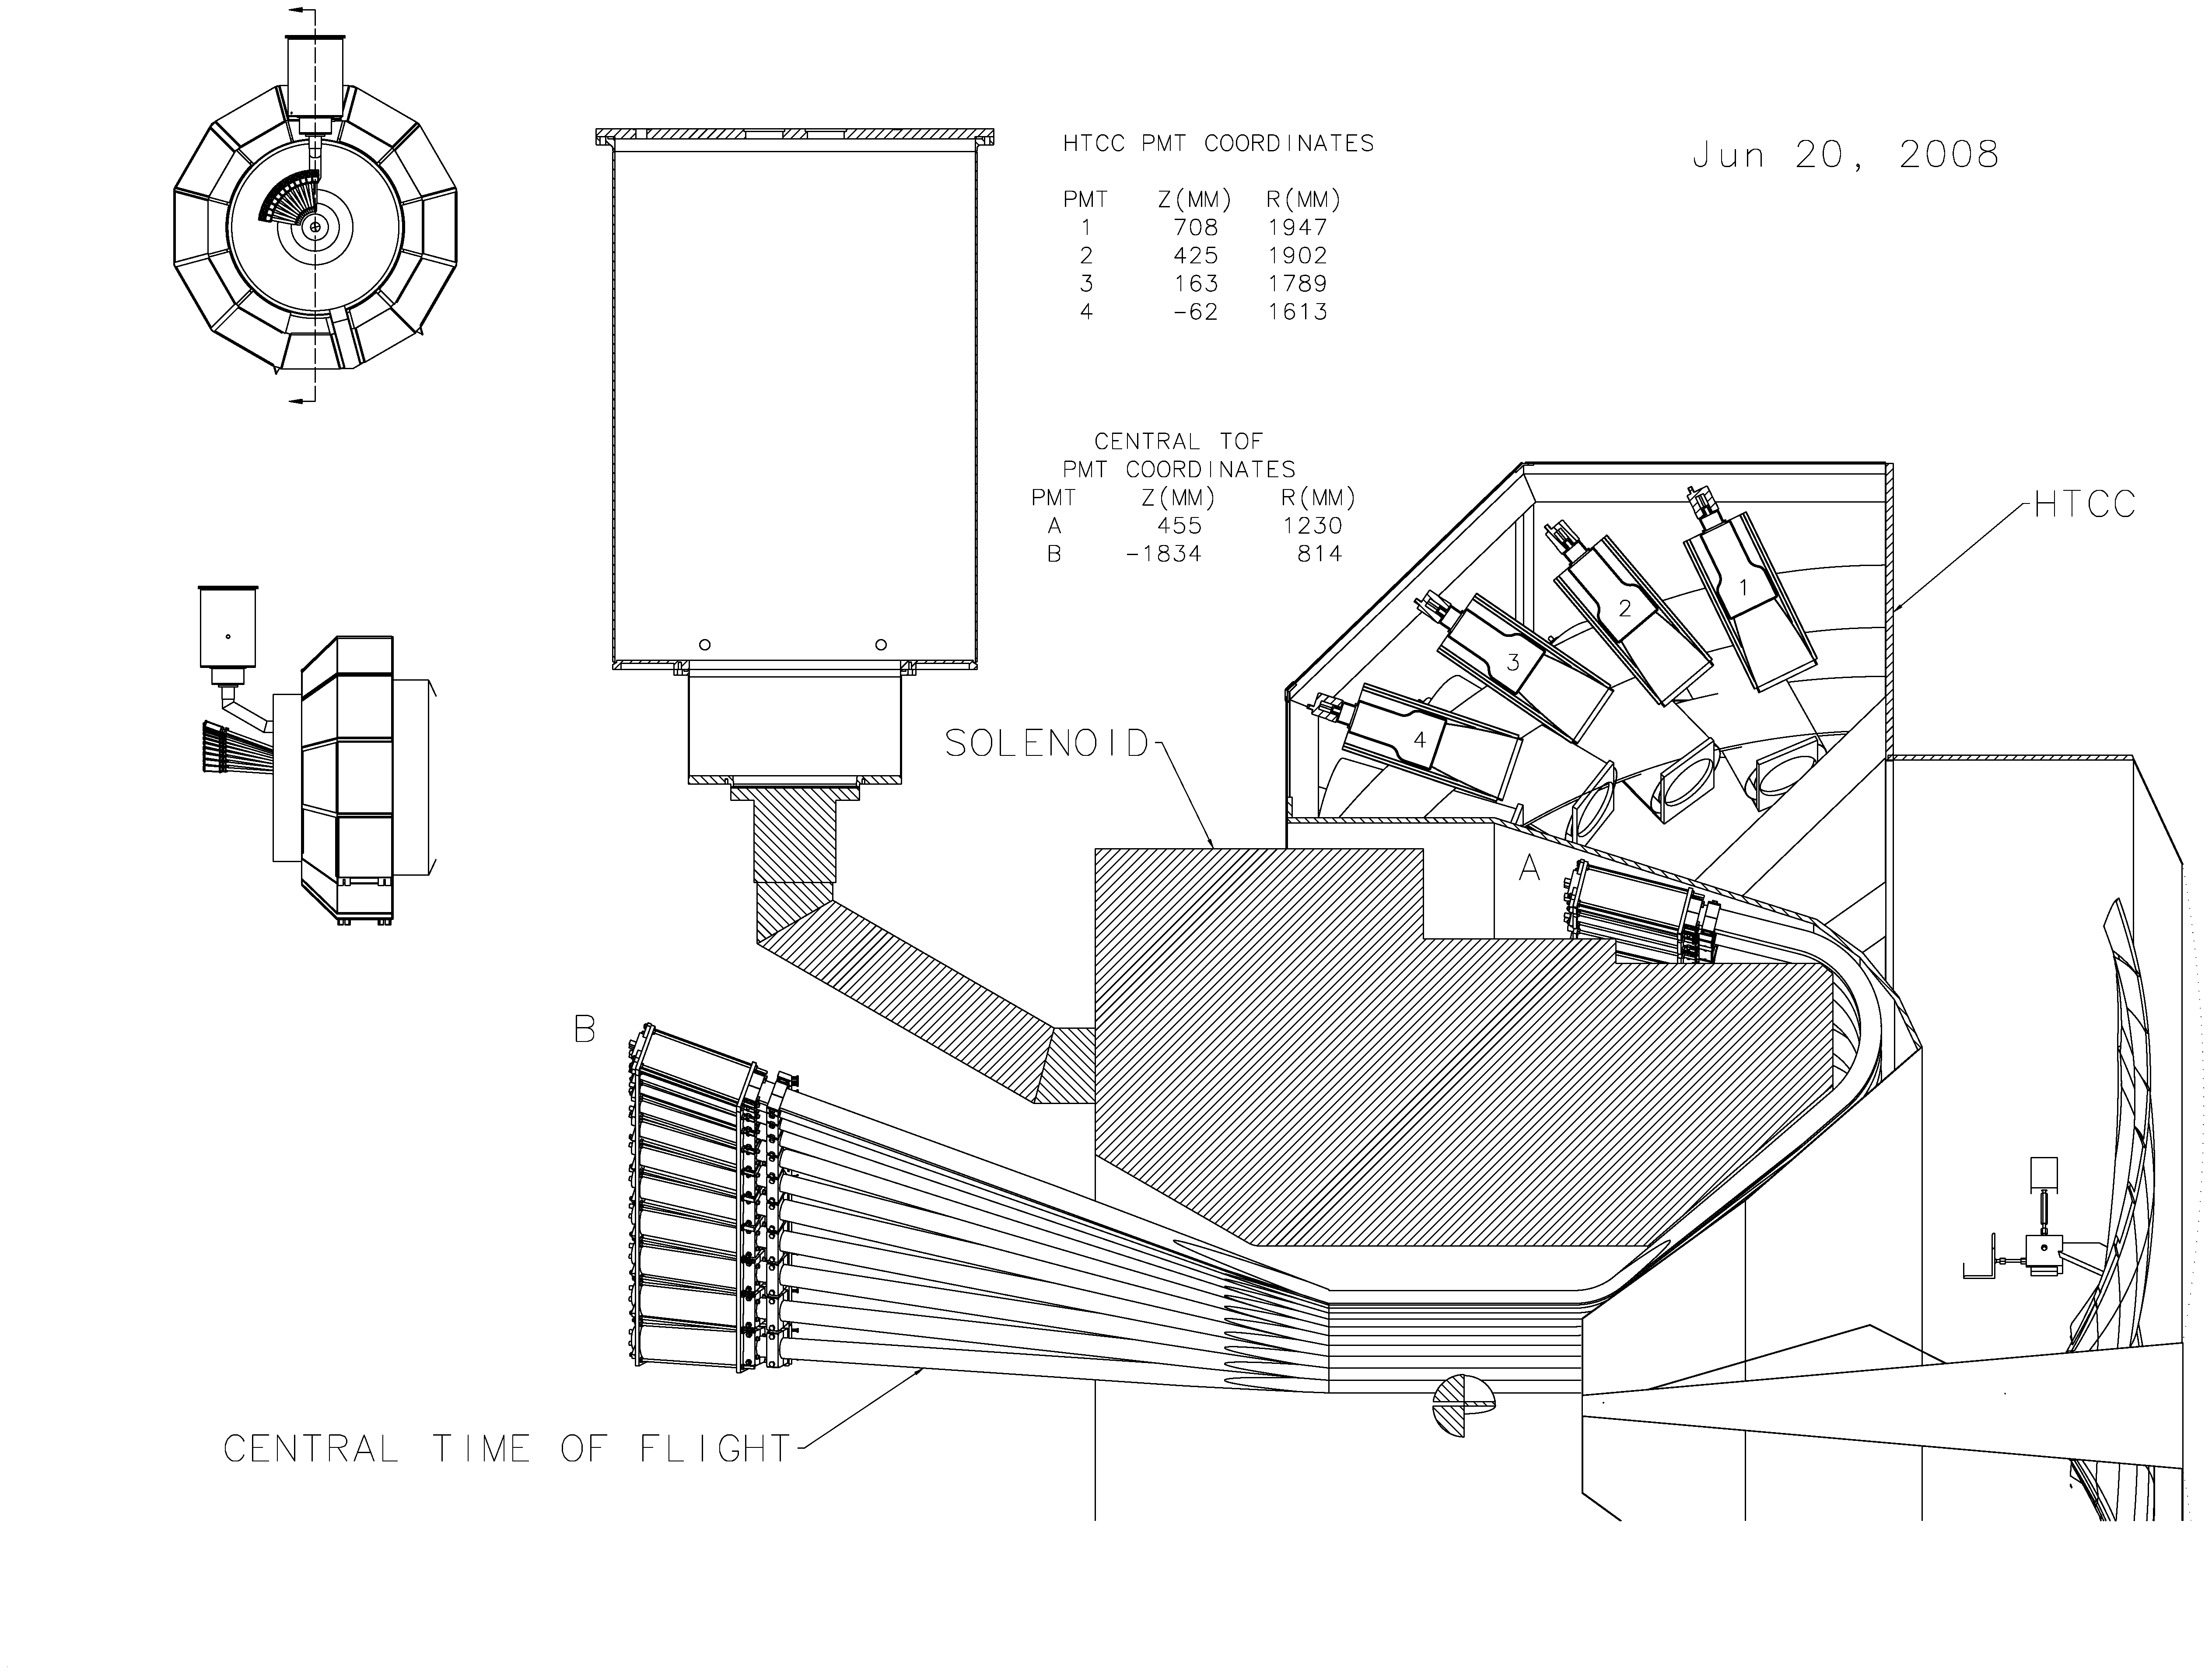
\includegraphics[width=.98\textwidth]{HTCC_CTOF_STUDY_060507_WRAP.eps}
\caption{\small{The layout of the {\tt CLAS12} central TOF detector.  
The solenoid is shown by the hatched area.  The scintillators form a barrel, 
66-cm long with an inner radius 24.945~cm.  At the upstream and downstream
ends, 50-mm diameter light guides are included that have a pitch of 
20$^\circ$ and 41$^\circ$, respectively.  The 1.4 -- 1.6-m long light guides 
for conventional PMTs may be replaced with $\leq$1-m long light guides to 
accommodate magnetic-field-immune photo-detectors.}}
\label{barrel2}
\end{figure}
%%%%%%%%%%%%%%%%%%%%%%%%%%%%%%%%%%%%%%%%%%%%%%%%%%%%%%%%%%%%%%%%%%%%%%%%%%%

%%%%%%%%%%%%%%%%%%%%%%%%%%%%%%%%%%%%%%%%%%%%%%%%%%%%%%%%%%%%%%%%%%%%%%%%%%%
\begin{figure}[htbp]
\centering
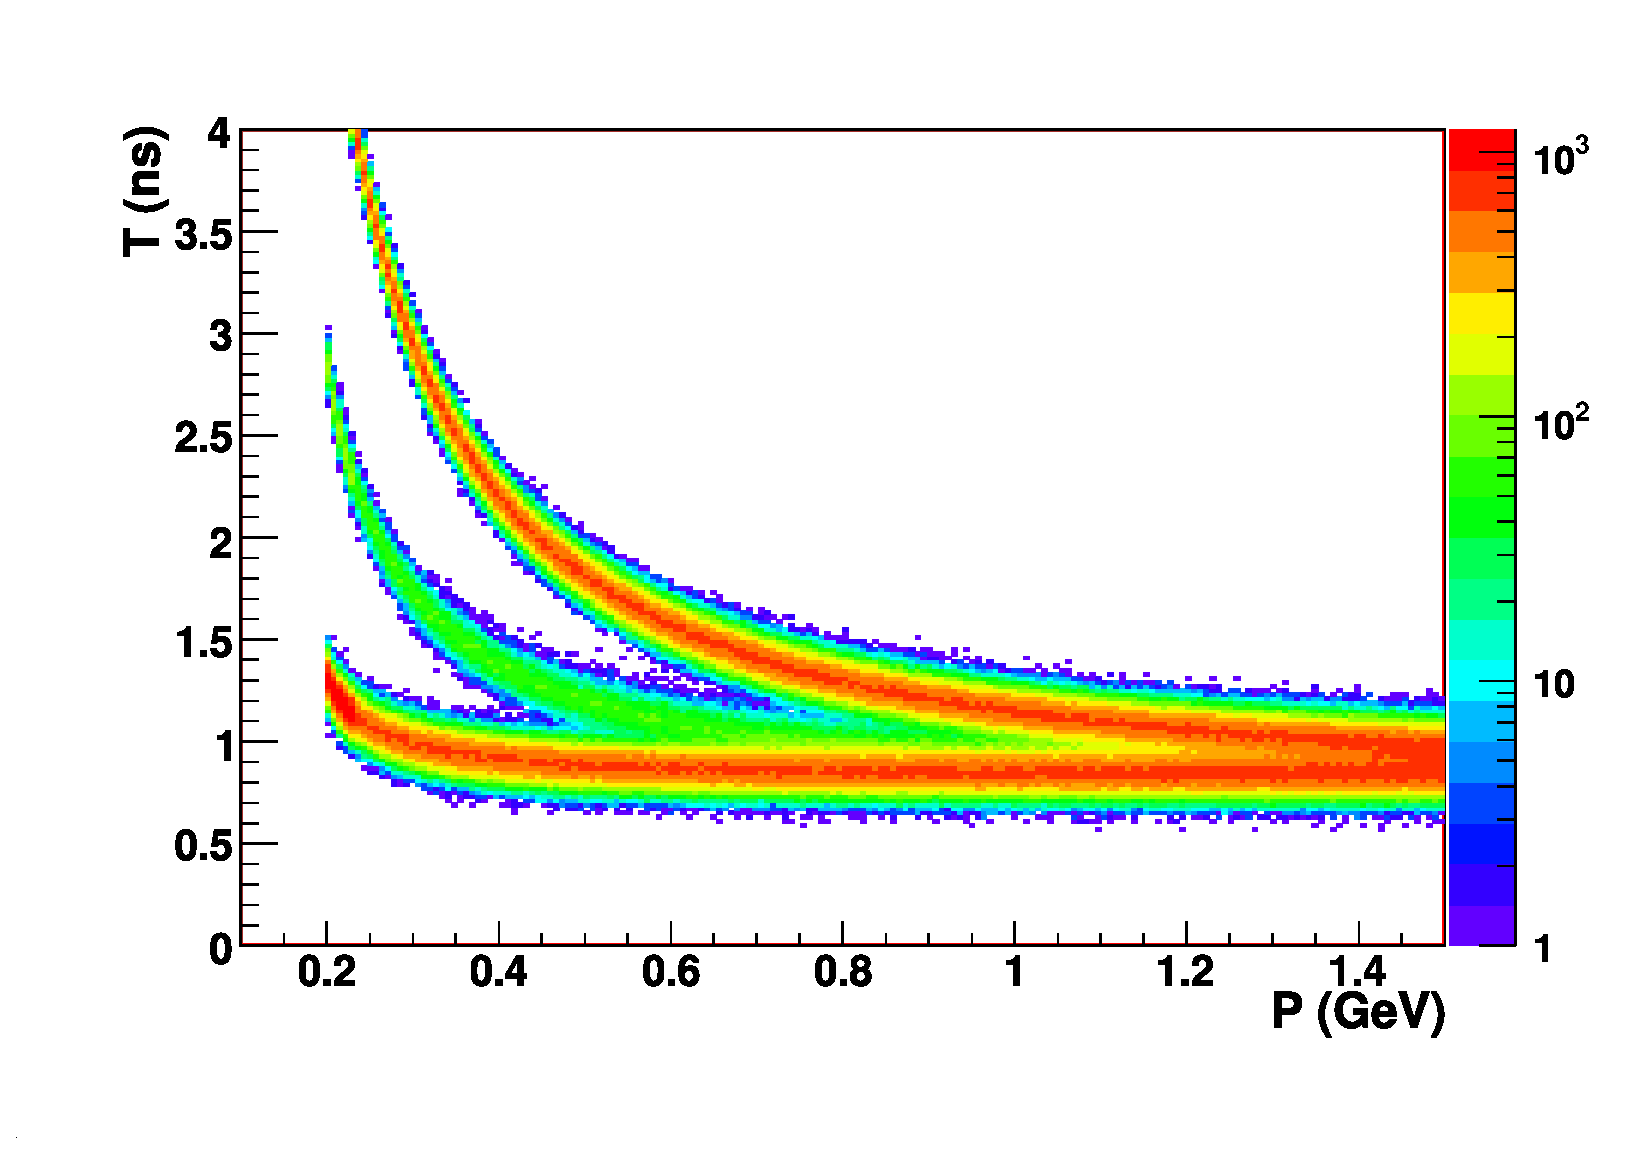
\includegraphics[width=0.7\textwidth]{ctof90deg.eps}
\caption{\small{Time of flight in the transverse direction vs. particle 
momentum for protons (top), kaons (middle), and pions (bottom).}}
\label{ctof_timing}
\end{figure}
%%%%%%%%%%%%%%%%%%%%%%%%%%%%%%%%%%%%%%%%%%%%%%%%%%%%%%%%%%%%%%%%%%%%%%%%%%%

The timing information in {\tt CLAS12}~\cite{r2} will be referenced to 
a stable radio-frequency signal from the accelerator.  Therefore, the 
time-of-flight resolution is determined as $\sigma_{TOF} = 0.5 \sigma_{PMT}$.
Thus we aim to develop a CTOF counter with an effective resolution of a
single photomultiplier, with $\sigma_{PMT} \leq 72$~ps.  We refer to 
$\sigma_{PMT}$ as an ``effective resolution'' since it is determined by 
the scintillator rise time ($\leq 1$~ns), light collection efficiency, 
discrimination, and the experimental environment, as well as by the 
excellent intrinsic timing characteristics of modern photomultipliers 
tubes (PMTs).

In our R\&D program we are following a conservative strategy, i.e. we 
are aiming for the best possible resolution using double-sided readout 
with conventional PMTs and very long light guides ($\leq 1.5$~m), delivering 
light to an area outside of the central solenoid where the associated 
magnetic fields are low (see Fig.~\ref{fig:mmap1}).

%%%%%%%%%%%%%%%%%%%%%%%%%%%%%%%%%%%%%%%%%%%%%%%%%%%%%%%%%%%%%%%%%%%%%%%
\begin{figure}[htbp]
\centering
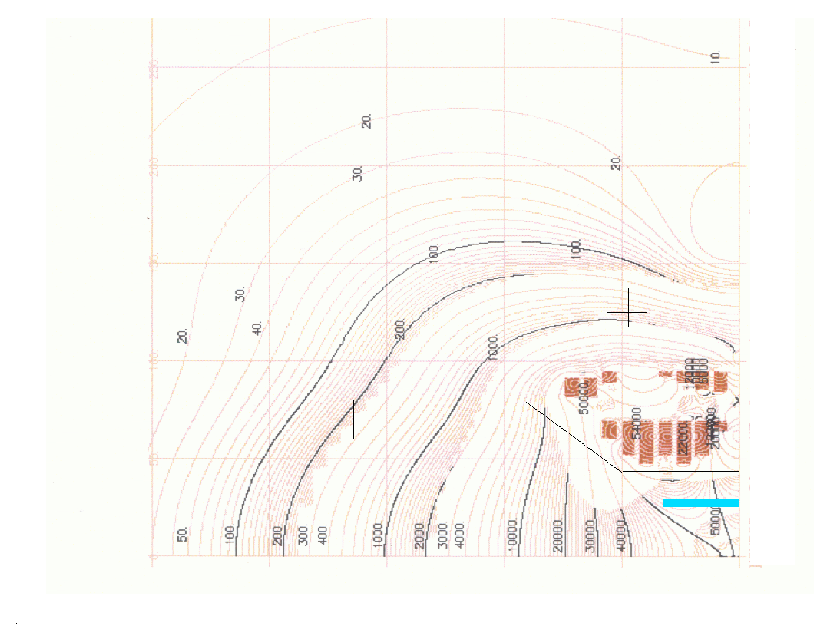
\includegraphics[width=0.9\textwidth]{mmap1.eps}
\caption{\small{Location of R2083 PMTs (cross-hairs) in relation to the 
magnetic field map for the central {\tt CLAS12} solenoid.}}
\label{fig:mmap1}
\end{figure}
%%%%%%%%%%%%%%%%%%%%%%%%%%%%%%%%%%%%%%%%%%%%%%%%%%%%%%%%%%%%%%%%%%%%%%%

We have proven both experimentally and with calculations that long light 
guides should have an increasing cross section moving from the scintillator
to the PMT.  This feature allows delivery of about twice as much light 
compared to a light guide of a constant cross section.  Therefore it is 
preferable to use PMTs with large photocathodes.  The actual length and 
configuration of the light guides will be defined by the maximum magnetic 
field that can be tolerated by a conventional PMT.  Bent light guides, shown 
on the downstream side of Fig.~\ref{barrel2}, will be used with ordinary PMTs, 
which have to be protected against magnetic fields $\leq 1000$~G.  On the 
upstream side magnetic fields are below 500~G.

In parallel, we are pursuing other possible solutions based on modern PMTs  
that are capable of operating in high magnetic fields, such as micro-channel
plate, fine-mesh, and metal-channel PMTs.  The review of possible candidates 
is given in Section~\ref{phdrev}.  At the current time, all of the aforementioned  
PMTs are being considered as options for the CTOF system. 

At the 5~T nominal solenoid field, long light guides of complex shape 
are unavoidable elements of the CTOF counter instrumented with both ordinary 
and/or fine-mesh PMTs. In order to investigate the design and technology for 
bent light guides (see Section~\ref{design2083}), we consider a realistic 
pilot design for the CTOF barrel with light guides shaped as a narrow pyramid.
In Section~\ref{mutchler} we focus on the design of long light guides and 
optimization of the light guides via Monte Carlo calculations.  Prototyping 
and reference measurements of $\sigma_{PMT}$ with ordinary and magnetic field 
insensitive photo-detectors are described in Section~\ref{measurements}.  
From our R\&D program, coupled with the results of detailed Monte Carlo 
calculations,  we estimate $\sigma_{PMT}$ for different possible CTOF 
designs (see Section~\ref{estimates}).

Within the program of employing magnetic-field-immune PMTs, we have measured 
the timing resolution of counters instrumented with micro-channel plate (MCP) 
PMTs with an on-board preamplifier.  We describe details of our measurements 
in Section~\ref{meas85011}.  Such PMTs are supposed to be attached directly to
the scintillators.  The corresponding pilot design is given in 
Section~\ref{des85011}.  However, the performance of MCP PMTs with on-board 
amplifiers is the subject of future tests in magnetic fields up to 4.5~T.

Another magnetic-field-immune ($\leq 1$~T) photo-detector is the fine-mesh
(FM) PMT.  We also plan to test more precise metal-channel (MC) PMTs for 
their performance in magnetic fields up to $\leq 0.2$~T with magnetic shielding.
Both types require significantly shorter ($\le$1~m) light guides to deliver 
light to the locations with a low enough field.

We emphasize that our conservative design with ordinary PMTs may accommodate 
new photo-detectors, provided the space reserved for the long light guides can 
be used to house the new PMTs.

\section{Counter Prototyping and Reference Measurements}
\label{measurements}

Several prototype scintillation counters were manufactured at Kyungpook 
National University (KNU) in 2004-2007.  In cooperation with the Detector 
Group at JLab, two reference counters were made with double-sided readout 
via MCP PMTs.  In all of our prototypes, we have used Bicron-408 
scintillators $2 \times 3 \times 50$~cm$^3$ in size.  Each prototype counter 
was instrumented with test PMTs on both ends for a double-sided readout.
The detailed description of the prototypes, test measurements, analysis 
methods, and results are published in several {\tt CLAS} notes and NIM 
papers~\cite{Baturin:2005,r1,llg,barb06}.

We have used two basic configurations for measuring the effective PMT time 
resolution.  Our main setup for express measurements consists of only one 
counter.  In order to measure the effective resolution of the PMTs, we placed 
a radioactive source on the surface of the scintillator.  Using the 
double-sided readout of the signal time and amplitude, we determined the 
location of the source via the difference between the arrival times of the
two signals.  The standard deviation of the determined source location is 
proportional to the product of $\sigma_{PMT}$ and the known effective speed 
of light in the scintillator.

For reference we use a triplet of identical counters exposed to cosmic rays.
The reference triplet consists of three identical scintillator bars with 
double-sided readout.  The spacing between the middle and top counters and the
middle and bottom counters was matched.  To determine the effective 
resolution of the PMTs we use the method of cosmic ray tracking.  The track 
coordinates are determined in each of the three counters via time difference 
measurements in each counter.  For each counter we also determine the time 
of a light flash in the scintillator as the mean value of the arrival times 
at both ends.  Thus we exclude coordinate-dependent delays caused by light 
propagation from the hit point to the PMTs.  For the straight tracks with 
constant velocity, the hit time of the middle counter equates to the mean 
value of the top and bottom hits.  This fact results from the simple geometry 
of the setup.  Therefore, the difference in timing between the top and
middle and the bottom and middle counters should be zero, while the 
distribution of the residual values is determined by fluctuations in the PMT 
timing.  In order to determine the effective $\sigma_{PMT}$, we study the 
distribution of the residuals.  The standard deviation of residuals is 
proportional to $\sigma_{PMT}$.

In our studies we have shown with different measurement methods
\cite{Baturin:2005,r1,barb06} that the effective time resolution of a 
Hamamatsu R2083 PMT attached directly to our test scintillators may be as 
good as $\approx$52~ps.  This value relates to a minimum ionizing particle 
energy deposition of $\approx$6.6~MeV in 3~cm of plastic.  However, if the 
1-m long light guides, shaped as a cut pyramid, mediate the light signal, 
then the resolution drops to $\approx$78~ps. 

The effective resolution of the Burle 85011 multi-anode (64 anodes) 
micro-channel plate PMT of $\approx$75~ps was measured using a single 
counter setup with the radioactive source method.  Amplification of the
PMT signal via an on-board amplifier, which was designed at JLab for 
this purpose, was required for these measurements.  The amplification 
allows the MCP to operate at a reduced gain, thus its counting rate 
capability is higher~\cite{Baturin:2005}.

Recently at Kyungpook National University~\cite{kuznetsov} we studied
a setup with six Hamamatsu R7761 fine-mesh PMTs attached directly to our 
reference scintillators.  With this setup we have determined the effective 
$\sigma_{R7761}$ to be $\approx$60~ps in the central region of the triplet.   
The method of time resolution measuring with the radioactive source was also 
used with a narrow 45-MeV proton beam incident on the center of our reference 
counter with double-sided readout.  The effective $\sigma_{R7761}$ was 
determined to be $\approx$34~ps. The full range of 45~MeV protons in plastic 
scintillator is 25~mm, therefore the protons stop completely in the scintillator.
However, due to the Birks effect, the energy deposition of 45-MeV protons is 
only $\approx$35~MeV.  We plan further studies with this setup to address the 
coordinate and angular dependence of the effective resolution.

Below we describe in more detail the studies with the setup of three counters
instrumented with six 1-m long light guides~\cite{llg} and single counters 
instrumented with Burle 85011 micro-channel plate PMTs and Hamamatsu R7761-70 
fine-mesh PMTs.

Comparing the various tests, we conclude that the effective time resolution of 
the PMTs in our prototypes is mostly dictated by the statistical fluctuations  
in the number of primary photoelectrons.  Therefore, we conclude that further 
progress in improving the effective time resolution may be provided with 
better light guide design and optical properties, better coupling of the PMTs 
to the light guides, and improved scintillator output in the corresponding 
wavelength area.

\subsection{Time Resolution Measurements with R2083 PMT Triplets}

Six light guides with our pyramid shape were manufactured at KNU.  The light 
transportation efficiency (LTE) of these light guides was found to be 
$LTE=0.44\pm0.04$ via Monte-Carlo calculations~\cite{mutch} and various 
measurements~\cite{llg}.  In order to increase the produced light, the 
orientation of the scintillators was changed to 3~cm along the cosmic particle 
track.  The obtained values of the effective $\sigma_{PMT}$ are listed in 
Table~\ref{crt} in comparison to other measurements at different conditions. 

%%%%%%%%%%%%%%%%%%%%%%%%%%%%%%%%%%%%%%%%%%%%%%%%%%%%%%%%%%%%%%%%%%%%%%%%%%%
\begin{table}[htbp]
\begin{center}
\begin{tabular}{|c|c|c|c|c|c|c|} \hline
  & Setup \& Method                & Year &lg(N)&$\Delta E$ (MeV) & $\sigma_{PMT}$(ps)& Status \\ \hline
1 & 2$\times$R2083,2cm,2$\times$LG(1 m)& 2004 &6    & $T_{\beta}<2.28$ &        &\small{Publ.}   \\
  & coordinate meth.;$^{90}$Sr   &      &  $vs~x$   & $\to$ 4.4        & 89.1$\pm$4.0        &                \\ \hline
2 & 2$\times$Burle 8501-501,NoLGs & 2004 &6 & $T_{\beta}<2.28$ & $\approx$80,    &\small{Publ.}   \\ 
  & coordinate meth.;$^{90}$Sr   &      &  $vs~x$   & $\to$ 4.4        & 125$\pm$4           &                \\ \hline
3 & 6$\times$R2083,2 cm,No LGs   & 2004 &6 & cosmic            &  &\small{Publ.}   \\
  & cosmic ray tracking            &    & $vs~x,\theta$  & $\approx$4.4     & 59.1$\pm$0.7       &                \\ \hline
4 & Same as \#3                    & 2005 &5 &                  &                     &\small{Publ.}   \\
  &                                &      &  $vs~x,\theta$ & $\approx$4.4     & 62.3$\pm$0.4       &                \\ \hline
5 & 6$\times$R2083, 3 cm, NoLGs    & 2005 &5 &                  &                     &\small{Publ.}   \\
  & cosmic ray tracking            &      &  $vs~x,\theta$ & $\approx$6.6     & 52.0$\pm$0.6       &                \\ \hline
6 & Same as \#5                    & 2006 &5 &                  &                    &\small{Publ.}   \\
  & \textbf{reference with no LG}  &      & $vs~x,\theta$  & $\approx$6.6     & \textbf{52.2$\pm$0.4}       &                \\ \hline
7 & 6$\times$R2083, 2 cm,          & 2005 &  &                  &                   &   \\
  & 2$\times$LG (1 m),             &      &5 & $\approx$4.4     & 92.3$\pm$0.5      &                \\
  & cosmic ray tracking            &      & $vs~x,\theta$  &                  &     &\small{Publ.}   \\ \hline
8 & 6$\times$ R2083, 3 cm,         & 2005 &5 &                  &                   &                \\
  & 2$\times$LG (1 m)              &      & $vs~x,\theta$  & $\approx$6.6     & 83.6$\pm$0.6       &\small{Publ.}   \\ \hline
9 & Same as \#8                    & 2006 &5 &                  &                    &                \\
  & \textbf{reference with LGs}    &      & $vs~x,\theta$  & $\approx$6.6     & \textbf{77.9$\pm$0.6}       &\small{Publ.}   \\  \hline
10& 2$\times$Burle 85011, NoLGs    & 2006 &6 & $T_{\beta}<2.28$ & 86.6$\pm 1;10^6$ s$^{-1}$ &              \\ 
  & coordinate method; $^{90}$Sr   &      & $vs~x$  & $\to$6.6         & 71.4$\pm 1;10^5$ s$^{-1}$ &\small{Publ.} \\ \hline
11& 2$\times$FM R7761-70, NoLGs    & 2007 &3 & cosmic           & $60-66$               &\small{Discon-}  \\ 
  & cosmic ray tracking            &      &$x\approx0$  & $\approx$6.6     &                &\small{tinued}       \\ \hline
12& 2$\times$FM R7761-70, NoLGs    & 2008 &3 & protons          & $\approx34$           & \small{In Progr.}  \\ 
  & cosmic ray tracking            &      & $x\approx0$ & $\approx$45      &                &              \\ \hline                  
\end{tabular}
\end{center}
\caption{\small{Reference measurements of the effective time resolution 
(standard deviation) of different PMTs.  The values of $\sigma_{PMT}$ in rows 
1--10 of this table are averaged over -25~cm$<x<$25~cm and 
-45$^\circ$ $< \theta <$45$^\circ$.  The uncertainties shown in this table 
are derived from the fitting procedures.  The possible systematic uncertainty 
is 6\% on the given values.}}
\label{crt}
\end{table}
%%%%%%%%%%%%%%%%%%%%%%%%%%%%%%%%%%%%%%%%%%%%%%%%%%%%%%%%%%%%%%%%%%%%%%%%%%%

The best $\sigma_{PMT}$=52~ps=$\sigma_{NLG}$ was obtained with our no light 
guide (NLG) setup (see Fig.~\ref{nlgres}), while with the 1-m long 
pyramid-shaped light guides (LLG), we have measured $\sigma_{PMT}$ = 77.9~ps 
= $\sigma_{LLG}$ (see Fig.~\ref{lgres}).  One can see from these two figures 
that $x$-dependent systematics in the residuals are significant only in the 
case of direct contact to the scintillators, while in the measurements performed 
with light guides, these effects are negligible. 

This systematic effect reflects a combination of at least two phenomena. 
The first one is the coordinate dependence of the effective speed of light in the  
scintillator bar.  The reason is that the closer the hit is to the PMT, the more d
irect light with higher longitudinal speed participates in the PMT signal developing 
at the threshold level.  The second effect is the well known time walk effects
associated with the discriminators.

However, if long light guides are implemented, then the direct light does not 
share in the signal build-up and the signal size becomes significantly longer 
due to the larger light path variations.  As one can see from Figs.~\ref{nlgres}
and \ref{lgres}, both effects are much less pronounced in the measurements with   
the long light guides.
 
%%%%%%%%%%%%%%%%%%%%%%%%%%%%%%%%%%%%%%%%%%%%%%%%%%%%%%%%%%%%%%%%%%%%%%%
\begin{figure}[htbp]
\centering
\includegraphics[width=0.8\textwidth]{cosmic-6pmtnlg_picture.ps}
\caption{\small{Effective time resolution of a PMT ($\sigma$) in the triplet 
without light guides.  (UL) scatter-plot of residuals vs. longitudinal 
coordinate $x$; the dashed line shows mean values, (UR) overall distribution of 
residuals, (LL) local $\sigma$ vs. $x$ with mean value $\sigma=52.2\pm0.4$~ps, 
(LR) ADC values.}} 
\label{nlgres}
\end{figure}
%%%%%%%%%%%%%%%%%%%%%%%%%%%%%%%%%%%%%%%%%%%%%%%%%%%%%%%%%%%%%%%%%%%%%%%

%%%%%%%%%%%%%%%%%%%%%%%%%%%%%%%%%%%%%%%%%%%%%%%%%%%%%%%%%%%%%%%%%%%%%%%
\begin{figure}[htbp]
\centering
\includegraphics[width=0.8\textwidth]{cosmic-6pmtllg_picture.ps}
\caption{\small{Effective time resolution of a PMT ($\sigma$) in the triplet 
with 1-m long straight light guides.  (UL) scatter-plot of residuals vs. 
longitudinal coordinate $x$ ;the dashed line shows mean values, (UR) overall 
distribution of residuals, (LL) local $\sigma$ vs. $x$ with mean value 
$\sigma=77.9\pm0.6$~ps, (LR) ADC values.}}
\label{lgres}
\end{figure}
%%%%%%%%%%%%%%%%%%%%%%%%%%%%%%%%%%%%%%%%%%%%%%%%%%%%%%%%%%%%%%%%%%%%%%%

To estimate the effective $\sigma_{PMT}$ in different counter designs (i.e. 
with different dimensions of the light guides, etc.) we use the above 
declared values and the empirical relations deduced from Monte Carlo 
simulations~\cite{mutch} for ``extrapolation'' of the measured $\sigma_{PMT}$ 
to the different designs.

We emphasize that the resolution with 1-m long light guides, $\sigma_{LLG}$, 
is worse due to the absorption of $\approx$56\% of the light in the light 
guides.  The amount of light at the photocathodes is proportional to the 
light transmission efficiency ($LTE$) of the light guides and, assuming the 
statistical nature of the resolution, we can estimate $\sigma_{LLG}$ as:

\begin{equation}
\frac{1}{\sqrt{LTE}}\sigma_{NLG} =\frac{1}{\sqrt{0.44}}\times52.2~{\rm ps}
=78.7~{\rm ps},
\label{eq31}
\end{equation}

\noindent
where $\sigma_{NLG}$ is the measured resolution.  The resulting value  
matches to the reference from row--9 of Table~\ref{crt} within a 1\% accuracy.
Therefore, we conclude that in our test setup the effective $\sigma_{PMT}$ 
is determined mostly by the statistics of the primary photoelectrons, i.e. 
by the amount of light at the photocathodes.  We use this experimental fact 
as the main rule in our further estimations of $\sigma_{PMT}$ in various 
environments.

\subsection{Time Resolution Measurements with a Burle 85011 PMT}
\label{meas85011}

For these measurements the new assembly of a Burle 85011 PMT with an 
``on-board'' preamplifier (with a gain value of $\times$50) and a high 
voltage divider that was designed at JLab was employed.  The design of the 
circuit board is described in Ref.~\cite{pa85011}.  This design follows the 
requirement implied by the final goal of $\sigma_{PMT}\le$72~ps in time 
resolution.

The Burle~85011 photocathode is formed by 64 pads $0.6\times0.6$~cm$^2$ in 
size.  We took into account the fact that the MCP PMT resolution may be 
limited by the signal propagation time through the pad, which is spread 
between 0 at the point of the pad-wire contact and $l_{max}/c$ for the most 
remote point, at the distance $l_{max}$.
  
We used the central $6\times6$ pads as a single photocathode.  In order 
to avoid additional jitter due to propagation from the individual pads, the 
central 36 pads were grouped into three amplification channels via isochronous 
transmitting lines.  The resulting three signals are summed up, also 
isochronously, at the last stage of amplification.  Thus we guarantee that 
the jitter caused by signal propagation is defined by the size of a single 
pad, which amounts to only 10~ps (i.e. negligible).

The test counter with our ``standard '' scintillator was assembled at KNU 
and resolution measurements with a radioactive source were recently performed.
We present the results below.

\paragraph*{Effective Time Resolution at the Ultimate Gain:}

A sample plot given by the coordinate method with extrapolation to the 
energy loss in a 3-cm thick scintillator is shown in Fig.~\ref{mcp85011sample}.
The extrapolated time resolution $\sigma_{PMT}$=71.4~ps was obtained at the 
ultimate MCP gain of $0.89\times10^6$.  This resolution is very close to our 
goal.  Unfortunately the counting rate at such a high gain is limited to 
$10^5s^{-1}$~\cite{Baturin:2005}.  Therefore, we have measured the resolution 
at lower gains and present below the measured dependence upon the MCP gain.  
Prior to determining the gain, one has to measure the number of primary 
photoelectrons ($N_{ppe}$) emitted from the photocathodes. 

%%%%%%%%%%%%%%%%%%%%%%%%%%%%%%%%%%%%%%%%%%%%%%%%%%%%%%%%%%%%%%%%%%%%%%%
\begin{figure}[htbp]
\centering
\includegraphics[width=0.8\textwidth]{esxm_picture13.ps}
\caption{\small{Effective time resolution of a Burle 85011 MCP PMT obtained 
with the location method of the $^{90}$Sr source placed in the center of the 
counter.  (UL) energy ($E$) spectrum of $\beta$-particles, (LL) coordinate 
distribution ($x$) of $\beta$-particles with $E>1$~MeV, (UR) $\sigma_x$ of 
the peak vs $E$, (LR) $<x>$ vs  $E$.}}
\label{mcp85011sample}
\end{figure}
%%%%%%%%%%%%%%%%%%%%%%%%%%%%%%%%%%%%%%%%%%%%%%%%%%%%%%%%%%%%%%%%%%%%%%%

\paragraph*{Number of Primary Photoelectrons in the MCP:}

We have measured the number of primary photoelectrons produced by MIPs using
the technique developed within the coordinate method~\cite{Baturin:2005}.
The PMT output signals were split in order that a fraction $f$=0.16 of 
the initial current fed the ADC inputs, while the rest triggered the 
corresponding discriminators.
 
The ADC spectrum of $\beta$-particles was then used to determine the number 
of primary photoelectrons and their dependence upon $\beta$-particle energy.  
The corresponding graphs are shown in Fig.~\ref{mcpnppe85011}.  These
results were extrapolated to determine the expected number of primary
photoelectrons in a 2-cm thick scintillator, which was found to be 
$N_{ppe}=370\pm8$ (note that this value relates to both photocathodes). This
result is in good agreement with expectations using the quantum efficiency
(QE) specified in the Burle 85011 data sheet. 

%%%%%%%%%%%%%%%%%%%%%%%%%%%%%%%%%%%%%%%%%%%%%%%%%%%%%%%%%%%%%%%%%%%%%%%
\begin{figure}[htbp]
\centering
\includegraphics[width=0.8\textwidth]{enppe_picture13.ps}
\caption{\small{Determination of the number of primary photoelectrons.  (UL) 
Energy ($E$) spectrum of $\beta$-particles, (UR) $N_{ppe}$ vs $E$.  We 
expect the number of primary photoelectrons to be $369 \pm 2$ for a MIP 
energy of $\approx$4.4~MeV, (LL) spectrum of $(e_l-e_r)$, where $e_{l,r}$ are 
the energies measured from the two sides of the counter, (LR) mean value of 
$(e_l-e_r)$ vs. $\beta$-particle energy.}}
\label{mcpnppe85011}
\end{figure}
%%%%%%%%%%%%%%%%%%%%%%%%%%%%%%%%%%%%%%%%%%%%%%%%%%%%%%%%%%%%%%%%%%%%%%%

\paragraph*{Measurements of the MCP Gain:}

The MCP gain ($G$) was determined using the measured $N_{ppe}$ and the
$\beta$-particle spectra measured with the ADCs as:

\begin{equation}
G = \frac{2 \times \alpha \times A_{0}}{f \times e \times N_{ppe} \times G_a},
\label{gain}
\end{equation}

\noindent
where $A_0$ is the pedestal-subtracted ADC value corresponding to the upper 
edge of the $\beta$-spectrum, $E_0$=2.28~MeV, $\alpha$ is the ADC channel 
width (0.25~pC), $G_a$ is the amplification factor of the preamplifier (50), 
$f$ is the aforementioned spitting factor, and $e$ is the charge of the
electron.  The factor of 2 in the numerator is from the number of 
photocathodes.  A plot of the determined gain as a function of the MCP 
voltage is shown in Fig.~\ref{hvvsgain85011}.

%%%%%%%%%%%%%%%%%%%%%%%%%%%%%%%%%%%%%%%%%%%%%%%%%%%%%%%%%%%%%%%%%%%%%%%
\begin{figure}[htbp]
\centering
\includegraphics[width=0.65\textwidth]{hvvsgain_picture85011.ps}
\caption{\small{High voltage vs. MCP gain.  Curves (1) and (2) are fits to 
a power law form.  (1)-left PMT, (2)-right PMT.}}
\label{hvvsgain85011}
\end{figure}
%%%%%%%%%%%%%%%%%%%%%%%%%%%%%%%%%%%%%%%%%%%%%%%%%%%%%%%%%%%%%%%%%%%%%%%

\paragraph*{Time Resolution vs. MCP Gain:}

We have measured the effective time resolution of a Burle 85011 PMT at 
different high voltage settings.  The resolution yielded by the coordinate 
method is shown in Fig.~\ref{sigmamip85011} as a function of the MCP gain. 
One can see that at a gain of $0.5\times10^5$, where the MCP can operate 
at a 1~MHz counting rate~\cite{Baturin:2005}, the effective time resolution 
with a 3-cm thick scintillator is only $86.6 \pm 1$~ps.  With this value we 
are 20\% away from our goal of 72~ps.  Thus a further significant 
improvement of $N_{ppe}$ is required.

%%%%%%%%%%%%%%%%%%%%%%%%%%%%%%%%%%%%%%%%%%%%%%%%%%%%%%%%%%%%%%%%%%%%%%%
\begin{figure}[htbp]
\centering
\includegraphics[width=0.62\textwidth]{res85011vsgain_picture85011.ps}
\caption{\small{Resolution of the Burle 85011 PMT vs. the MCP gain ($G$).  
The circles are for $\sigma$ at $\Delta E$=2.28~MeV.  The squares are for 
$\Delta E$=6.6~MeV (which corresponds to MIPs in a 3-cm thick scintillator). 
The curves are fits to the $G^{-2}$ dependence.  The amplification factor 
of the PMT signals is 50.}}
\label{sigmamip85011}
\end{figure}
%%%%%%%%%%%%%%%%%%%%%%%%%%%%%%%%%%%%%%%%%%%%%%%%%%%%%%%%%%%%%%%%%%%%%%%

\subsection{Measurements with Fine-Mesh Photomultipliers}
\label{secfinemesh}

Using the same triplet technique as for the R2083 PMTs, we have measured 
$\sigma_{PMT}$ of the fine-mesh PMTs.  In our standard counter triplet
\cite{Baturin:2005,llg} the ordinary PMTs in the middle counter were 
replaced with 27-mm Hamamatsu R7761 fine-mesh PMTs.  All PMTs were in 
direct contact with the scintillators.  The corresponding 
$\sigma_{R7761}$=64~ps is shown in Fig.~\ref{finemesh01} in comparison to 
the Hamamatsu R2083 PMTs.  It was further improved to $\approx$60~ps 
with cuts in the central region of the triplet instrumented with R7761 
PMTs and identical discriminators~\cite{kuznetsov}.

%%%%%%%%%%%%%%%%%%%%%%%%%%%%%%%%%%%%%%%%%%%%%%%%%%%%%%%%%%%%%%%%%%%%%%%
\begin{figure}[htbp]
\vspace{8.0cm}
\special{psfile=tau041007.eps hscale=45 vscale=45 hoffset=0 voffset=-15}
\special{psfile=tau0117a.eps hscale=45 vscale=45 hoffset=235 voffset=-15}
\caption{\small{Spectra of the 6 PMT time residuals scaled by $2/\sqrt{3}$.
Left panel: distribution with two R7761-70 PMTs and four R2083 PMTs (right).  
Right panel: distribution obtained with six R2083 PMTs.  The actual effective
$\sigma_{R7761}$=64~ps is derived from the RMS width of the left panel.  The  
reference $\sigma_{R2083}=52 \pm 1$~ps from the right panel coincides with 
the previously reported value from Table~\ref{crt}.}}
\label{finemesh01}
\end{figure}
%%%%%%%%%%%%%%%%%%%%%%%%%%%%%%%%%%%%%%%%%%%%%%%%%%%%%%%%%%%%%%%%%%%%%%%

The time residual spectrum  at the center of the reference counter
instrumented with two R7761-70 PMTs is shown in Fig.~\ref{finemesh02}.  
It was obtained with the 45-MeV proton beam at an $\approx10^5s^{-1}$ 
counting rate \footnote{For details see KNU presentation 
http://www.jlab.org/$\sim$baturin/KNUpresentation0208.pdf.}.  Protons completely 
stop in the bulk of the scintillator, therefore the deposited energy is 
$\approx$10 times higher than the reference MIP energy deposition.  The standard 
deviation $\sigma$=24~ps of this distribution translates into 
$\sigma_{R7761}\approx 34$~ps for a single PMT.  In order to compare this result 
to our reference from Table~\ref{crt} (line 5), this value has to be scaled to 
the reference energy 6.6MeV by a factor of $\sqrt{(45~{\rm MeV}/6.6~{\rm MeV})}$.  The 
additional  factor of $\sqrt{0.77}
$\footnote{This number was obtained from 
the paper\\
T.J. Gooding and H.G. Pugh. Nucl. Instr. and Meth. 7 (1960), p. 189.\\
see also \\
R.L. Craun and D.L. Smith. Nucl. Instr. and Meth. 80 (1970), p. 239.}
accounts for the reduced light output of 45-MeV protons due to Birks effect.
Since PMTs were attached directly to the scintillator, the effective PMT area was reduced by a 
factor of $\approx$0.8. All of this results in the following preliminary  
resolution of:

\begin{equation}
\sigma_{R7761} \approx 34~{\rm ps} \times \sqrt{\frac{45}{6.6} \times 0.77 \times 0.8 }
= 70~{\rm ps}.
\label{eq776}
\end{equation}

\noindent
However, the uncertainty on this value has to be determined experimentally. 
This result was obtained in direct contact to the scintillator and the proton 
beam hit the center of the counter, where the left and right signals are almost 
identical.  Therefore, effects related to the signal shapes cancel out.

In this test, one PMT signal was used as a TDC ``start'', while another provided
the TDC ``stop''.  Therefore, all events were concentrated within a few TDC channels. 
In this situation, the differential nonlinearity of the TDC, which may be as high as 
15\%, directly affects the measured time resolution.   
     
Therefore, further studies of differential nonlinearity effects, as well as of 
coordinate and angular dependence with realistic light guides, are required in order 
to establish the ultimate effective time resolution of the fine-mesh PMTs.
 
%%%%%%%%%%%%%%%%%%%%%%%%%%%%%%%%%%%%%%%%%%%%%%%%%%%%%%%%%%%%%%%%%%%%%%%
\begin{figure}[htbp]
\vspace{8.0cm}
\special{psfile=KNU45MEV.eps hscale=100 vscale=100 hoffset=110 voffset=-15}
\caption{\small{The time residual spectrum at the center of the reference 
counter obtained with R7761 fine mesh PMTs with a 45-MeV proton beam.  The 
standard deviation is $24.2\pm0.6$~ps.}}
\label{finemesh02}
\end{figure}
%%%%%%%%%%%%%%%%%%%%%%%%%%%%%%%%%%%%%%%%%%%%%%%%%%%%%%%%%%%%%%%%%%%%%%%

\section{Review of Modern Photo-Detectors}
\label{phdrev}

Different possible approaches to the design of the {\tt CLAS12} CTOF
counter are considered below in relation to the advantages and disadvantages 
of different photo-detectors. 

\subsection{Ordinary Dynode PMTs}

Following our conservative strategy, we will maintain our effort to achieve 
the desired timing resolution with ordinary Hamamatsu R2083 PMTs.  The gain 
and timing characteristics of R2083 PMTs are very good for this purpose (see 
Table~\ref{table1PMTS}).  However, for ordinary PMTs there is no other option 
than to be placed outside of the region of high magnetic field.  Therefore, 
$\approx$1.5-m long light guides are required to deliver the light to an area 
with $B \le 30$~mT.  Shorter light guides will require a heavy magnetic shield 
composed of 3 concentric cylinders.  In addition, according to the preliminary 
design shown in Fig.~\ref{barrel2}, the light guides on the downstream side 
will have to be bent by $139^\circ$.  This reduces the net light at the PMT,
the ultimate limit of which is dictated by the desired time resolution.  
Therefore significant progress is required in the light guide design and 
manufacturing technique.

%%%%%%%%%%%%%%%%%%%%%%%%%%%%%%%%%%%%%%%%%%%%%%%%%%%%%%%%%%%%%%%%%%%%%%%%%%%
\begin{table}[htbp]
\begin{center}
\begin{tabular}{|l|r|r|r|r|r|r|}   \hline
PMT Model Characteristics       & R2083      &  H8500     & R6504 & R5924  & R7761   & 85011        \\ 
                                & Dynode     &   MC       & FM    &  --    &   --    &  MCP         \\ \hline  
Photocathode sizes, mm         & $d$=46     &$49\times49$& $d$=51& $d$=39 & $d$=27  & $49\times49$ \\ \hline
Anode configuration             & 1          & $8\times8$ &   1   &  --    &   --    & $8\times8$   \\ \hline
Area ratio PMT/SC (9.6~cm$^2)$  & 1.77       &  2.19      & 2.14  & 1.24   & 0.6     & 2.19         \\ \hline
Wavelength max. response, nm    & 420$\pm$80 &    --      & --    & --     & --      & 400$\pm$80   \\ \hline
-//-  at 10\% of max. QE, nm    & $300-650$  &    --      & --    &  --    & --      & --           \\ \hline
Window thickness, mm            &  1         &    1.5     &  1    &   --   &  --     &  2           \\ \hline
Number of stages                & 8 dyn.     &  12dyn.    & 19 fm &   --   &  --     & 2MCP         \\ \hline
Photocathode material          & Bi-alk.    &    --      &  --   &   --   &  --     & --           \\ \hline
Photocathode radius, mm        & 55         &   flat     &  --   &   --   &  --     & --           \\ \hline
Sensitivity@420nm, $\mu$A/lm    & 80         &   55       &  70   &   --   &  --     & 55           \\ \hline
Sensitivity in blue, $\mu$A/lm  & 10         &   8        &  9    &  --    &  --     & 8            \\ \hline
Quantum efficiency@420mn        & .22        &   0.2      &  0.22 &  0.22  & 0.22    & 0.12         \\ \hline
Anode rise time, ns             & 0.7        &   0.8      &  2.7  & 2.5    & 2.3     & 0.3          \\ \hline
Transit time ($t_T$), ns        & 16         &   6        &  11   & 9.5    &  7.5    & 4            \\ \hline
$t_T$ spread (FWHM), ps         & 370        &   400      & 470   &  440   &  350    & 80           \\ \hline
Gain$\times$10$^{-6}$           & 2.5        &   1        &  10   &   --   &   --    & 0.5          \\ \hline
Dark current, nA                & 100        &    32      &    50 &   50   &  30     & 1            \\ \hline
\end{tabular}
\end{center}
\caption{\small{Technical data of the R2083 PMT from Hamamatsu in comparison with 
other candidates.}}
\label{table1PMTS}
\end{table}
%%%%%%%%%%%%%%%%%%%%%%%%%%%%%%%%%%%%%%%%%%%%%%%%%%%%%%%%%%%%%%%%%%%%%%%%%%%%%%%%%

\subsection{Micro-Channel Plate Photomultipliers}

An alternative solution with micro-channel plate (MCP) PMTs is very attractive
for the following reason.  Due to the immunity of MCPs to magnetic fields, 
proven up to $\leq 2$~T\cite{kich}, micro-channel plate PMTs could be 
attached directly to the scintillators.  Therefore, the mechanical design of 
the barrel may be significantly simpler.  The intrinsic timing properties of 
MCP PMTs are perfect.  The properties of one such photomultiplier (Burle 
85011) are shown in Table~\ref{table1PMTS}.
  
The single photon timing resolution (see Fig.~\ref{mcpt}) remains below  
$\sigma_{TTS}$=35~ps up to $\approx$2~T and perhaps higher fields.  The 
gain (see Fig.~\ref{mcpg}) also does not degrade in such high magnetic 
fields~\cite{kich}.

%%%%%%%%%%%%%%%%%%%%%%%%%%%%%%%%%%%%%%%%%%%%%%%%%%%%%%%%%%%%%%%%%%%%%%%%%%%
\begin{figure}[htbp]
\centering
\includegraphics[width=0.65\textwidth]{fig02MC.ps}
\caption{\small{Transition time spread of the MCP PMT vs. magnetic field.}}
\label{mcpt}
\end{figure}
%%%%%%%%%%%%%%%%%%%%%%%%%%%%%%%%%%%%%%%%%%%%%%%%%%%%%%%%%%%%%%%%%%%%%%%%%%%

%%%%%%%%%%%%%%%%%%%%%%%%%%%%%%%%%%%%%%%%%%%%%%%%%%%%%%%%%%%%%%%%%%%%%%%%%%%
\begin{figure}[htbp]
\centering
\includegraphics[width=0.65\textwidth]{fig01MC.ps}
\caption{\small{Gain of the MCP PMT vs. magnetic field at different 
orientations.}} 
\label{mcpg}
\end{figure}
%%%%%%%%%%%%%%%%%%%%%%%%%%%%%%%%%%%%%%%%%%%%%%%%%%%%%%%%%%%%%%%%%%%%%%%%%%%

Unfortunately, the quantum efficiency of MCP PMTs is about one-half that of 
ordinary PMTs, which has a direct adverse effect on the TOF resolution.
However, very good resolution of a MCP photo-detector was already shown in 
Fig.~\ref{mcpt}.  In addition, it was shown~\cite{vavra} recently that the 
effective $\sigma_{PMT}$ of a Burle 85011 may be as good as 70~ps in a 
magnetic field up to 1.5~T.  In our aforementioned measurements, we have   
achieved a resolution of $\approx$75~ps, which is almost sufficient for our 
goals.  

Hence, the two approaches look almost equivalent with respect to the timing 
resolution.  The advantage of a R2083 PMT with its higher quantum efficiency 
is compensated by the loss of about half of the light in the light guides.
Almost nothing can be done with the quantum efficiency of MCP PMTs unless the 
PMT design is completely changed.

In the design with long light guides, we can try to optimize the light guides 
via Monte Carlo simulations for a maximum possible $LTE$, including the 
solution with PMTs capable of operating in moderate magnetic fields of 
$\approx$0.5~T.  In addition, we can use more refractive materials, such as 
Lexan.  It has a refractive index equal to that of the scintillators.  However, 
its attenuation length is higher.  Thus the gain in resolution may be achieved 
with relatively short light guides (0.5~m -- 1~m).

\subsection{Fine-Mesh and Metal-Channel Photomultipliers}
\label{fimemech}

The light deficiency problem may be solved with fine-mesh (FM) PMTs, 
which have been shown to operate at $\leq 1$~T or metal-channel (MC) PMTs,
provided they can be shown to operate well in fields up to 0.2~T with a proper 
shield.  The light guides can be about a factor of two shorter and we can use 
all of the experience that we have obtained with the design implementing the 
long light guides (see Section~\ref{design2083}). 

\paragraph{Fine-Mesh PMTs:}

In fine-mesh PMTs, the conventional dynode system is replaced with a ladder  
of fine-grade metal mesh at a certain potential.  The gain and resolution
\cite{kich} of a fine-mesh PMT vs. magnetic field are shown in 
Figs.~\ref{fmg} and \ref{fmt}, respectively.

%%%%%%%%%%%%%%%%%%%%%%%%%%%%%%%%%%%%%%%%%%%%%%%%%%%%%%%%%%%%%%%%%%%%%%%%%%%
\begin{figure}[htbp]
\centering
\includegraphics[width=0.65\textwidth]{fig03MC.ps}
\caption{\small{Gain of the R2490-05 fine-mesh PMT vs. magnetic field at 
different orientations.}} 
\label{fmg}
\end{figure}
%%%%%%%%%%%%%%%%%%%%%%%%%%%%%%%%%%%%%%%%%%%%%%%%%%%%%%%%%%%%%%%%%%%%%%%%%%%

%%%%%%%%%%%%%%%%%%%%%%%%%%%%%%%%%%%%%%%%%%%%%%%%%%%%%%%%%%%%%%%%%%%%%%%%%%%
\begin{figure}[htbp]
\centering
\includegraphics[width=0.65\textwidth]{fig04MC.ps}
\caption{\small{Transition time spread of the R2490-05 fine-mesh PMT vs. 
magnetic field.}}
\label{fmt}
\end{figure}
%%%%%%%%%%%%%%%%%%%%%%%%%%%%%%%%%%%%%%%%%%%%%%%%%%%%%%%%%%%%%%%%%%%%%%%%%%%

The behavior of modern FM PMTs R5505, R7761, and R5924 from Hamamatsu has 
been recently studied in magnetic fields up to 1.2~T~\cite{fmtr01}.  The 
generic time resolution of the 2-in R5924 PMT ($\approx$60~ps) was found 
unchanged up to a field of $\approx$0.8~T.  This characteristic was measured 
with light pulses equivalent to $\approx$300 photoelectrons.  In our recent
measurements, in which Hamamatsu R7761 FM PMTs were in direct contact with 
the scintillator, we also have achieved a similar time resolution~\cite{kuznetsov}. 

The counter instrumented with two fine-mesh PMTs attached to a 1-m long 
scintillator was tested in Ref.~\cite{foucher}.  This counter may be 
considered as a rough approximation a single element of the CTOF system.  
For this setup with a 6-cm thick Bicron-408 scintillator, we estimated 
$\sigma_{TOF}\approx 70$~ps.  The effective timing resolution of fine-mesh 
PMTs of $\sigma_{FM} \approx 63$~ps may be extracted from the data obtained
\cite{csn1} with  $50 \times 2 \times 5$~cm$^3$ Bicron-408 and 
$\approx$50-cm long light guides.

The closest in size to the R2083 PMT is the R6504 fine-mesh PMT (see
Table~\ref{table1PMTS}) from Hamamatsu with a QE $\approx$ 20\% at 420~nm.  
We emphasize that with expanding light guides (toward the PMTs), we gain 
about a factor of two in light collected at the PMT~\cite{llg}.  Therefore, 
PMTs with wide enough photocathodes are required to accommodate this design.  
Unfortunately, this PMT is already discontinued.  The timing characteristics 
of the R5924 PMT are almost the same, but it has a two times smaller sensitive 
area.  However, it is still larger than the scintillator cross section, therefore 
we plan to test it.  The R7761 PMT has almost a twice smaller sensitive area
(5.6~cm$^2$) compared to the size of the scintillator cross-section (9.6~cm$^2$). 
Therefore, it is  unlikely to collect enough light with realistically long light 
guides of 0.7--0.8~m length.  The reason is that even without attenuation, the 
transmittance of a light guide cannot exceed 0.58.\footnote{This is the ratio of 
the PMT area to the input area, which limits the acceptance due to phase space 
conservation.}

Unfortunately, the rise time of the R6504/R5924 PMT signal is $\approx$4 
times longer than that of the R2083 PMT.  In addition, the transition time 
spread is 100~ps higher than the 370~ps for the R2083.  We plan to measure 
the resolution of the R5924 PMT in addition to smaller FM tubes, metal-channel 
PMTs, the R2083 PMT, and MCP PMTs, using the same test setup and methods.

\paragraph{Metal-Channel Photomultipliers:}

Another interesting photo-detector worthwhile to investigate as a 
component of the CTOF counter is the metal-channel PMT, such as the
H8500 or R7400 PMTs from Hamamatsu.  The H8500 is a 64-channel PMT with a 
square photocathode.  The dynode system is formed by channels in  
precisely machined metal sheets.  Such PMTs have excellent timing 
characteristics, which are very close to that of the R2083 PMT, i.e. 
$\sigma_{TTS} \approx$400~ps, QE$\approx$ 20\%, and they have a high gain 
(see Table~\ref{table1PMTS}).

In our future tests we are going to verify whether such PMTs can operate at 
fields of $\leq$0.2~T with appropriate shielding.  This photo-detector may 
be a good candidate for further consideration in combination with light guides 
of moderate length.  

\subsection{Silicon Photomultipliers}

In recent years a variety of semiconductor devices (see Table~\ref{apd}) have 
been developed for light detection.  Their advantage of operating in high 
magnetic fields and with a small size detecting element is very attractive for 
designers of TOF systems.  A matrix of such detectors, with arbitrary dimensions, 
could be attached directly to the scintillators inside the magnetic field.  

%%%%%%%%%%%%%%%%%%%%%%%%%%%%%%%%%%%%%%%%%%%%%%%%%%%%%%%%%%%%%%%%%%%%%%%%%%%
\begin{table}[htbp]
\begin{center}
\begin{tabular}{|c|c|c|c|c|c|c|} \hline
APD name      & Size         & Drift dist.   & FWHM & $\sigma_t$ & Rate & QE \\ 
              &   mm         & $\mu$m & ps   & ps       &    s$^{-1}$       & 420 nm \\ \hline
5343          & $d$=1        & 10     & 82   & 35  & $10^7$ & 1-5\%  \\ \hline
5344~LC       & $d$=3        & 20     & 160  & 68  &        & 1-5\%  \\ \hline
SPL~2625      & $d$=3        & 120    & 1300 & 550 & $10^7$ & 1-5\%  \\ \hline
Beveled Edge  &              &        &      &     &        & 1-5\%  \\
LAAPD         & $d$=16       & 40     & 400  & 115 &        & 1-5\%  \\ \hline
30719         & $5\times5$   & 10     & 170  & 72  &        & 1-5\%  \\ \hline
C~30626       & $5\times5$   & 100    & 800  & 340 &$10^7$  & 1-5\%  \\ \hline
C~30703       & $10\times10$ & 180    & 1600 & 680 &        & 1-5\%  \\ \hline
SiPM          & $3\times3$   & 0      & 155  & 66  &$10^7$  &14-20\% \\ \hline
MPPC S10362-33-10C& $3\times3$   & 0  & 200  & 85  &$10^7$  &70\% \\ \hline
\end{tabular}
\caption{\small{Semiconductor device characteristics.}}
\label{apd}
\end{center}
\end{table}
%%%%%%%%%%%%%%%%%%%%%%%%%%%%%%%%%%%%%%%%%%%%%%%%%%%%%%%%%%%%%%%%%%%%%%%%%%%

A silicon photomultiplier~\cite{dolgo} is a $3 \times 3$~mm$^2$ matrix of 
5625 pixel photodiodes ($30 \times 30$~$\mu$m$^2$) with a common output. 
The photodiodes operate in the Geiger regime of bulk carrier amplification.  
Therefore, an almost immediate (no drift required) signal from a single 
photon may be seen with a standard shape and amplitude ($\approx$2.5~mV).  
The time resolution of a SiPM may be as high as 66~ps~\cite{dolgo} with 
3-mm thick BC-418 scintillator.  It is very important that the output may 
be triggered by the first arriving ``direct'' photons.  However, the noise 
at the nominal operating voltage is as high as $10^5-10^6$. 

The QE is a product of the pixel packing efficiency ($\approx$0.5) and the
Geiger mode efficiency ($\approx$0.6).  At 420~nm, the quantum efficiency
is $\approx$14\%, and it is likely that this may be improved to reach the 
QE of ordinary photo-detectors.  In addition, the signal has a tail 
$\approx$5~$\mu$s long.  Thus the recovery time may be as high as 5~$\mu$s.  
However, due to the large number of pixels, the SiPM count rate capability 
of light flashes with $\approx$500 photons, for example, is limited by a
rate of $\approx 10^7$~s$^{-1}$, which is typical for conventional PMTs.  
Nevertheless the optical cross-talk may significantly reduce its count rate 
capability.  For use in {\tt CLAS12}, the SiPMs would have to reside in a  
high radiation environment.  Therefore, their radiation hardness has to be 
addressed.  Due to all of the above reasons, SiPMs may be considered as a
candidate for future studies and an upgrade possibility for the {\tt CLAS12} 
CTOF system.
 
\subsection{Avalanche PhotoDiodes}

In the avalanche photodiode~\cite{apd}, the carriers are drifting with a 
velocity of 0.1~$\mu$m/ps toward the narrow region in which the avalanche 
develops. In such a device, the single photon time resolution is determined 
by the drift distance $x$, thus, roughly, $\sigma_{APD}\propto x$.  In 
addition, the dependence on the sizes is quite significant.  For example, 
the $x$=10-$\mu$m thick device 5343, roughly 1~mm in diameter, manifested a 
time resolution $\sigma \approx 35$~ps, while the $5\times5$~mm$^2$ 30719 
$x$=10-$\mu$m thick device shows $\sigma\approx$72~ps.  The thicker the 
device the higher is its QE, but the worse its time resolution.  The related 
parameters of available APDs are listed in Table~\ref{apd}.  The quantum 
efficiency of such a photo-detector is roughly 2\% -- 5\% in the region of 
BC-408 emittance, while for longer wavelengths, it may be as high as 70\%. 
In addition, their gain is quite low ($\approx10^4$) and amplification is 
required.  The behavior in a high radiation environment is not determined yet.
Therefore, at the present time, such photo-detectors may be considered as 
unlikely candidates for use in the {\tt CLAS12} CTOF system.

\section{Pilot Design with Conventional R2083 PMTs}
\label{design2083}

This design is based on a traditional and well-established approach of using 
ordinary photomultipliers coupled to scintillators via long light guides.
Hamamatsu R2083 PMTs have excellent timing characteristics.  In order to 
approach our goal for the effective $\sigma_{R2083}$=72~ps, we have been 
developing long (1~m) light guides of non-trivial shape with significantly 
improved light transmission efficiency ($\approx$44\%).  Also we are thinking 
about implementing a better light guide manufacturing approach using cast Acrylic,
which is a widespread technology for commercial applications.  The advantage of 
cast Acrylic is that the product has a near-perfect surface.  Thus, time-consuming 
polishing is not required.  In addition, we will keep an eye on the progress in 
organic materials with a refractive index close to that of scintillators, such as 
commercially available Lexan.   

\subsection{Detector Specification and Design Criteria}
\label{sbasval}

The nominal CTOF design, which starts with ordinary R2083 phototubes, may 
accommodate other types of photo-detectors, such as magnetic-field-immune 
micro-channel, fine-mesh, or more sensitive metal-channel phototubes of 
similar sizes.  The only thing that would have to be done in the design is
to change the lengths (cross section) of the corresponding light guide at 
the PMT side.  However, the space reserved for the light guides in the 
design has to be wide enough to accommodate these PMTs.  The independent 
parameters that determine the design of a single CTOF counter, including its 
light guides, are listed in Table~\ref{basval}.

%%%%%%%%%%%%%%%%%%%%%%%%%%%%%%%%%%%%%%%%%%%%%%%%%%%%%%%%%%%%%%%%%%%%%%%%%%%
\begin{table}[htbp]
\begin{center}
\begin{tabular}{|l|c|} \hline
Diameter of PMT in $\mu$-metal case        & 60~mm       \\
Diameter of the PMT photocathode          & 46~mm       \\
Number of scintillators                    & 50          \\
Thickness of scintillator along $r$-axis   & 31.5~mm     \\
Inner radius of the  barrel                & 25.0~cm     \\
Lengths of the scintillator barrel         & 66~cm       \\
Length of Upstream light guides            & 130--140~cm \\
Length of Downstream light guides          & 150--160~cm \\
The downstream opening angle               & $\pm 36^\circ$ \\\hline
\end{tabular}
\caption{\small{Basic values determining the CTOF counter design.}}
\label{basval}
\end{center}
\end{table}
%%%%%%%%%%%%%%%%%%%%%%%%%%%%%%%%%%%%%%%%%%%%%%%%%%%%%%%%%%%%%%%%%%%%%%%%%%%

The CTOF barrel has to be as hermetic as possible.  Therefore, due to the 
cylindrical symmetry of the setup, all elements of a single counter, 
including the scintillator, both downstream and upstream light guides, and 
PMTs, all have to fit into a $\phi$ range of 7.2$^\circ$ in the 
$(r,\phi)$-plane.  A schematic view of such a counter is shown in 
Figs.~\ref{bentlg03} and \ref{bentlgud03}.

%%%%%%%%%%%%%%%%%%%%%%%%%%%%%%%%%%%%%%%%%%%%%%%%%%%%%%%%%%%%%%%%%%%%%%%%%%%
\begin{figure}[htbp]
\centering
\includegraphics[width=0.7\textwidth]{JLABt0R2083-2.ps}
\caption{\small{The pilot design of the {\tt CLAS12} CTOF counter.
(1) R2083 PMT from Hamamatsu, (2) Acrylic light guides, (3) scintillators,
and (4) supporting cones and rings. The magnetic field is shown by the
vectors.}}
\label{bentlg03}
\end{figure}
%%%%%%%%%%%%%%%%%%%%%%%%%%%%%%%%%%%%%%%%%%%%%%%%%%%%%%%%%%%%%%%%%%%%%%%%%%%

%%%%%%%%%%%%%%%%%%%%%%%%%%%%%%%%%%%%%%%%%%%%%%%%%%%%%%%%%%%%%%%%%%%%%%%%%%%
\begin{figure}[htbp]
\centering
\includegraphics[width=0.7\textwidth]{bentlgupdownstream.ps}
\caption{\small{Upstream (1) and downstream (2) view of the CTOF detector.}}
\label{bentlgud03}
\end{figure}
%%%%%%%%%%%%%%%%%%%%%%%%%%%%%%%%%%%%%%%%%%%%%%%%%%%%%%%%%%%%%%%%%%%%%%%%%%%

\subsubsection{Scintillator Dimensions}

The length of the scintillators is predefined to be 50~cm.  Other dimensions  
of the scintillator are determined by the total number of counters 
(predefined as 50) and the inner radius of the scintillating barrel 
(predefined as 25~cm).  The scintillator cannot be a rectangular bar due to 
the cylindrical geometry of the setup.  The cross section of the scintillator 
is shown in Fig.~\ref{sccross}.  Since a single counter has to fit into a 
sector $2\gamma=7.2^\circ$, the cross section of the scintillator has to be a 
symmetric trapezoid with the sizes 31.46~mm and 35.4~mm for the bottom and 
top sides, respectively, and 31.5~mm high.  In this figure the trapezoid is 
inscribed into the cross section of the photocathode of the R2083 PMT.  

%%%%%%%%%%%%%%%%%%%%%%%%%%%%%%%%%%%%%%%%%%%%%%%%%%%%%%%%%%%%%%%%%%%%%%%%%%%
\begin{figure}[htbp]
\centering
\includegraphics[width=0.7\textwidth]{t0sccross.ps}
\caption{\small{The cross section of the scintillator inscribed into the 
photocathode of the R2083 PMT from Hamamatsu.  Light guides will join the
PMTs via the cylindrical side of the same diameter as the R2083 photocathode,
i.e. 46~mm.}} 
\label{sccross}
\end{figure}
%%%%%%%%%%%%%%%%%%%%%%%%%%%%%%%%%%%%%%%%%%%%%%%%%%%%%%%%%%%%%%%%%%%%%%%%%%%

\subsubsection{Dimensions of the PMT Housing}

In this design we assume that R2083 PMTs from Hamamatsu will be used, and 
that they will be housed in a metal case 60~mm in diameter.  This 
determines the divergence of the upstream light guides.  It is clear that 
50 adjacent PMTs with the specified diameter will form a ring of 
$\approx 50\times (60+10)~{\rm mm}/\pi = 111.4$~cm in diameter (we add 
10~mm to the diameter of the PMT case as tolerance).  With this number we set 
the radius of the ``PMT area'' $R_{PMT}$=55~cm.  Note, that it is not possible 
to place 50 adjacent PMTs, mounted on the ends of 1-m long light guides, 
at an $r$-coordinate below $R_{PMT}$. 

\subsubsection{Dimensions of the PMT Photocathode}

In the hermetic configuration, the expanding light guide has to match the 
cross section of the scintillator from one side.  At the PMT end, it has 
to match the photocathode of the PMT.  Therefore, it is natural to 
manufacture the ``pyramid'' light guides from Acrylic cylinders with a 
diameter of 46~mm, corresponding to the diameter of the R2083 PMT
photocathode.

\subsection{Light Guides} 

From the PMT-end, the 1-m long light guide has to match the circular 
photocathode of the PMT.  Therefore, light guides will be manufactured 
from Acrylic cylinders $\ge 46$~mm in diameter, which is the specified diameter 
of the R2083 PMT photocathode.  From the opposite side, it has to match 
the trapezoidal cross section of the scintillator.

It was shown via Monte Carlo calculations~\cite{mutch} that the light 
transportation efficiency depends significantly on the length of the 
cylindrical part of the light guide.  The corresponding dependence upon 
the length of the non-cylinder part of a 1-m long light guide is shown in 
Fig.~\ref{plgef}.

%%%%%%%%%%%%%%%%%%%%%%%%%%%%%%%%%%%%%%%%%%%%%%%%%%%%%%%%%%%%%%%%%%%%%%%%%%%
\begin{figure}[htbp]
\centering
\includegraphics[width=0.6\textwidth]{transitionvscyl.ps}
\caption{\small{The light transportation efficiency (vertical scale) of the 
``pyramid'' light guide vs. the length (horizontal scale) of the milled 
surface.}}
\label{plgef}
\end{figure}
%%%%%%%%%%%%%%%%%%%%%%%%%%%%%%%%%%%%%%%%%%%%%%%%%%%%%%%%%%%%%%%%%%%%%%%%%%%

The design of the upstream light guide is shown in Fig.~\ref{lgupstream}. 
The sides of the cylinder will be milled to form a wedge up to a radius of 
36.55~cm in the $(r,\phi)$-plane in order to fit into the 
$\Delta \phi=7.2^\circ$ sector.  The straight cylindrical parts will be longer
in order to deliver light to the area of $B<30$~mT.  Therefore at the nominal 
field $B$=5~T, the total length of the light guide will be $\approx$1.5~m.
 
The scintillator ends of the light guides will be further machined in order 
to form focusing mirrors on the inner and outer surfaces, respectively. 
Such machining is also necessary to form a trapezoid at this end for coupling 
to the scintillator.

%%%%%%%%%%%%%%%%%%%%%%%%%%%%%%%%%%%%%%%%%%%%%%%%%%%%%%%%%%%%%%%%%%%%%%%%%%%
\begin{figure}[htbp]
\centering
\includegraphics[width=0.7\textwidth]{t0lgupstr.ps}
\caption{\small{The design of the upstream light guide.}}
\label{lgupstream}
\end{figure}
%%%%%%%%%%%%%%%%%%%%%%%%%%%%%%%%%%%%%%%%%%%%%%%%%%%%%%%%%%%%%%%%%%%%%%%%%%%

%%%%%%%%%%%%%%%%%%%%%%%%%%%%%%%%%%%%%%%%%%%%%%%%%%%%%%%%%%%%%%%%%%%%%%%%%%%
\begin{figure}[htbp]
\centering
\includegraphics[width=0.7\textwidth]{t0lgdown.ps}
\caption{\small{The design of the downstream 1-m long light guide.}}
\label{lgdownstream}
\end{figure}
%%%%%%%%%%%%%%%%%%%%%%%%%%%%%%%%%%%%%%%%%%%%%%%%%%%%%%%%%%%%%%%%%%%%%%%%%%%

\subsection{Downstream Light Guides}

From the PMT-end, the light guide will match the circular photocathode of 
the PMT.  Therefore, the light guides will be manufactured from bent Acrylic 
rods of corresponding diameter.  From the opposite side, it has to match the 
trapezoidal cross section of the scintillator.  In addition, these light 
guides have a pitch of 45$^\circ$ relative to the scintillator to provide an 
immediate opening for forward-going particles.  Another complication is that 
these light guides have to be bent twice by 45$^\circ$ and 90$^\circ$, 
respectively.
 
The pilot design of the downstream light guide is shown in Fig.~\ref{lgdownstream}. 
The mirrors at the scintillator end will be milled similarly to the upstream 
light guide.  The minimum length of this light guide will be $\approx$1.6~m, 
provided the magnetic field at the PMT end will be $\le$50~mT at a nominal 
field $B$=5~T.

\section{PMT Magnetic Shields}
 
The main CTOF design is based on using ordinary PMTs coupled to the 
scintillators via $\approx$1.5-m-long light guides of a complex 
design\footnote{We anticipate that at the final design stage, regular 
PMTs may be replaced with fine-mesh PMTs with two times shorter light 
guides.  These PMTs are insensitive to fields up to 5000~G.}.  Our reference  
PMT is the 51-mm R2083 PMT from Hamamatsu.  It has a spherical photocathode 
in order to equalize the travel distances of the primary photoelectrons and 
is quite similar to the Phillips XP4312 PMT, which is 76~mm in diameter, hence 
it is less sensitive to magnetic fields.  The XP4312 PMT was thoroughly studied 
in 1993 by J.~Flint and E.~Smith as a candidate for the {\tt CLAS} TOF detectors
\footnote{J.~Flint and E.~Smith, ``Tests of Phillips XP4312/D1 PMTs in a Magnetic 
Field'', CLAS-Note-94-008.}.  It manifests an additional time smearing of 
$\sigma \approx 30$~ps at fields of 0.25--0.4~G at the photocathode, which 
corresponds to an external field of 30~G, reduced by the 1-mm thick $\mu$-metal 
shield that is 80~mm in diameter\footnote{See the corresponding field map in Fig.~13 
of CLAS-Note-94-008.}.  Since our PMT is similar in design, we can estimate that
the maximum field at the photocathode would be 0.2--0.4~G.

Two kinds of PMT shielding are possible in principle: passive and active shielding. 
Active shielding means using a solenoid around the PMT to cancel the internal field.  
We do not plan on using active shielding because, firstly, in our case, the fringe  
fields are not solenoidal, and secondly, such shields would be more complex and more 
costly, and thirdly, it may be a source of additional electronic noise.

With passive shielding, a diamagnetic superconducting cylinder could be used to 
block the magnetic field inside the cylinder.  Such shielding would be very complex 
and expensive, as well as requiring cryogenics for cooling.

Therefore, we plan to study a traditional approach based on the properties of 
ferromagnetic cylinders.  In such shielding, the magnetic field lines are 
concentrated in the bulk of a ferromagnet, reducing the fringe fields inside the 
cylinder.  However, the efficiency of such shielding at high fields is limited by 
the effect of saturation.

We plan to achieve field reduction to the 0.25-G level with a shield composed of 
three concentric ferromagnetic cylinders.  The important parameter in the CTOF 
design, is the external diameter $D_{s}$ of the magnetic shield.  This parameter
is determined by the radial coordinate $r_{50}$ of the 50 adjacent shields:

\begin{equation}
\label{dsmax}
D_{s} = 2\frac{r_{50}}{\sin(3.6^\circ)} = 134.277 \times r_{50}.
\end{equation}

The characteristics of the PMTs relevant to the design of the magnetic shields
are given in Table~\ref{PMT_char}.

%%%%%%%%%%%%%%%%%%%%%%%%%%%%%%%%%%%%%%%%%%%%%%%%%%%%%%%%%%%%%%%%%%%%%%%%%%%
\begin{table}[htbp]
\begin{center}
\begin{tabular}{|c|c|c|c|c|c|c|c|c|c|}  \hline 
PMT     & $D_{pm}$ & $S_a$  & $L_{m}$ & $B_{t}$  & $M$         & $r_{50}$ & $D_{sm}$ & $L_{LG}$ & $B_{o}$   \\
        & mm       & mm$^2$ &  mm     & G        & kg          & mm      &          &  mm       & G         \\ \hline
R2083-u & 54       & 1662   & 120     & 0.25     & $\approx$5  & 826     &  88.     & 1400      & $\le500$  \\ \hline
R2083-d & --       &  --    & --      & --       & $\approx$10 & 1090    & 146.4    & 1600      & $\le1000$ \\ \hline
H8500-u & 72       & 2400   & 15      & $\le500$ & $\approx$10 &  596    &  80.1    & 945       & 2000      \\ \hline 
H8500-d & --       &  --    & --      &  --      & $\approx$10 & 890     & 119.5    & 945       & 3000      \\ \hline
\end{tabular}
\end{center}
\caption{\small{Characteristics of the PMTs relevant to the CTOF magnetic
shield design.}}
\label{PMT_char}
\end{table}
%%%%%%%%%%%%%%%%%%%%%%%%%%%%%%%%%%%%%%%%%%%%%%%%%%%%%%%%%%%%%%%%%%%%%%%%%%%

\noindent
Here,

\begin{itemize} 
\item $D_{pm}$ - nominal diameter of the PMT; 
\item $S_a$    - PMT sensitive area;
\item $L_{m}$  - maximum length to protect against the magnetic field;
\item $B_{t}$  - maximum tolerated field by the ``naked'' PMT;
\item $M$      - expected shield mass; 
\item $r_{50}$ - radial coordinate according to the current design;
\item $D_{sm}$ - maximum possible diameter of the PMT shield via Eq.(\ref{dsmax});
\item $L_{LG}$ - shortest possible light guide length in current design;
\item $B_{o}$  - magnetic field at the PMT location at the specified light guide length.
\end{itemize}

According to this table, the upstream R2083 PMTs have to withstand against 
a field $\leq 500$~G, provided the light guide length is 1400~mm.  In this case, 
the diameter of the magnetic shield has to be below 88~mm.  The downstream 
R2083 PMT meets a significantly higher non-uniform magnetic field.  Provided 
the downstream light guide length is 1600~mm, the maximum field would be 
$\leq 1000$~G, while the magnetic shield diameter may be as high as 146~mm. 

The metal-channel H8500 PMT may operate at 200~G without magnetic shielding.
However, with a powerful enough shield,  both kinds of PMTs could operate at  
higher fields.  In such a situation, shorter light guides could be used,
which would lead to an improved resolution. 

R2083 PMTs will be used in the assembly H2431, enclosed into the 200-mm long,
0.8-mm thick $\mu$-metal of 60~mm external diameter.  However, we plan to 
change the H2431 design in order to arrange a overhang of 50--60~mm from the 
photocathode side.  This is required for a more efficient shielding design
\footnote{The internal field drops significantly at a depth of one radius of 
the shield.}.

\subsection{Ferromagnetic Shielding}

In ferromagnetic shields, the field lines are concentrated in the bulk of 
the ferromagnetic, thus reducing the fringe fields inside the protecting  
area.  The problem with infinite hollow ferromagnetic cylinders in uniform 
transverse magnetic fields may be solved analytically\footnote{See E.~Smith,
GlueX-doc-843.}, as well as the problem of ellipsoids in axial fields.  
Therefore, the following practical formulas are recommended by the Magnetic 
Shield Corporation for rough estimates of magnetic shield parameters:

\begin{equation}
S = \frac{B_o}{B_{in}}\approx \mu({B_m})\frac{t}{D_+}~~~;
~~~B_m \approx B_o\frac{D_+}{0.8t}~~~;
~~~t\approx B_o\frac{D_+}{0.8B_m},
\label{eq000}
\end{equation}

\noindent
where $S$ is the shielding factor of a cylinder, $\mu(B_m)$ is the 
permeability as a function of the field $B_m$ in the shielding material,
$B_o$ is the external field, $B_{in}$ is the field inside the 
ferromagnet, $t$ is the thickness of the shielding material, and $D_+$ 
is the external diameter of the cylinder.  For a set of separated coaxial 
cylinders, the shielding factor may be estimated as the product of 
the individual factors.

\subsubsection{Finite Element Analysis}

Two external layers are the most important element for shield performance.  
Therefore, we have analyzed a double-layer magnetic shield against 3000~G.  The 
parameters of such a pilot shield are listed in Table~\ref{ca001}. 

%%%%%%%%%%%%%%%%%%%%%%%%%%%%%%%%%%%%%%%%%%%%%%%%%%%%%%%%%%%%%%%%%%%%%%%%%%%%%%%%%%
\begin{table}[htbp]
\begin{center}
\begin{tabular}{|c|c|c|c|c|c|c|c|c|c|} \hline
Cyl & $B_{o}$  & $D_+$ & $D_-$ & $t$ & $B_m$ & $\approx\mu$ & $S$  & $B_{in}$ & $Fm$      \\ 
$n$ &  G       & mm    & mm    & mm  & G     &              &      & G        &           \\ \hline  
1   & 3000     & 136   &   86  & 25  & 20000 & 600          & 40   & 80       & Netic     \\ \hline
2   & 80       &  84   &   80.8& 1.6 & 5300  & 150000       & 2850 & 0.03     & Hiperm-49 \\ \hline
\end{tabular}                                                      
\end{center}
\caption{\small{Two-layer shield design parameters. $n$ - layer number starting 
from the external layer, $B_{o}$ - external field, $D_+$ - external diameter, 
$t$ - ferromagnetic thickness from Eq.(\ref{eq000}), $B_m$ - field in the 
ferromagnetic from Eq.(\ref{eq000}), $\mu$ - permeability from the magnetization 
curve, $S$ - shielding factor, $B_{in}$ - field inside the shielding or the external 
field for a next layer, and $Fm$ - ferromagnetic material.}}
\label{ca001}
\end{table}
%%%%%%%%%%%%%%%%%%%%%%%%%%%%%%%%%%%%%%%%%%%%%%%%%%%%%%%%%%%%%%%%%%%%%%%%%%%%%%%%%%
\clearpage

The result of the finite element analysis (FEA) calculations\footnote{Calculations 
were performed by the Mu-shield Company (D.~Grilli).} in a perpendicular field is 
shown in Fig.~\ref{GRILLI}.  According to this plot, the minimum field inside 
the shield is 0.23~G, which is 15 times higher than the naive estimate from  
Table~\ref{ca001}.  This means that the interaction between layers is 
important and has to be analyzed via more advanced FEA calculations.

%%%%%%%%%%%%%%%%%%%%%%%%%%%%%%%%%%%%%%%%%%%%%%%%%%%%%%%%%%%%%%%%%%%%%%%%%%%
\begin{figure}[htbp]
\centering
\includegraphics[width=.8\textwidth]{magshieldGrilli-1.ps}
\caption{\small{Sample of a field map for the 2-layer PMT shield in the 
3000~G external field.  The field in the center is 0.23~G.}}
\label{GRILLI}
\end{figure}
%%%%%%%%%%%%%%%%%%%%%%%%%%%%%%%%%%%%%%%%%%%%%%%%%%%%%%%%%%%%%%%%%%%%%%%%%%%

In Fig.~\ref{VBT3CY}, the pilot design of a 3-layer shield is shown.  A very high 
permeability Netic will be used for the external layer.  For the middle layer, 
Hiperm-49 may be used, since it has higher permeability at lower fields.  For the 
inner shielding, a very soft Co-Netic may be considered.  The dimensions will be 
further optimized via FEA calculations. 

%%%%%%%%%%%%%%%%%%%%%%%%%%%%%%%%%%%%%%%%%%%%%%%%%%%%%%%%%%%%%%%%%%%%%%%%%%%
\begin{figure}[htbp]
\centering
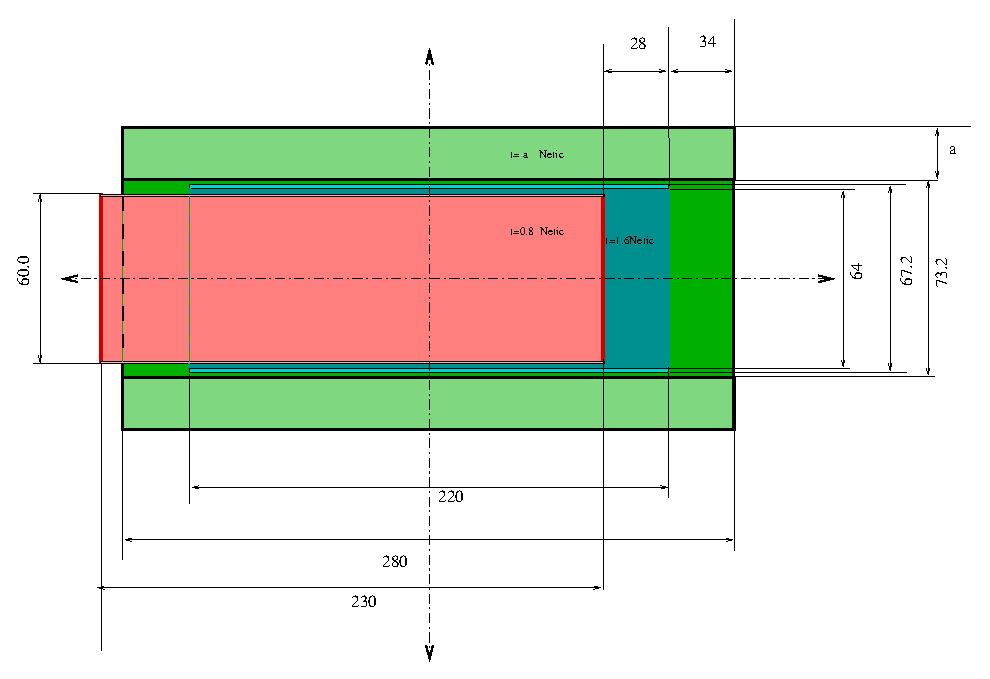
\includegraphics[width=1.0\textwidth]{R2083-3000-ph.eps}
\caption{\small{Pilot design of the PMT magnetic shield.}}
\label{VBT3CY}
\end{figure}
%%%%%%%%%%%%%%%%%%%%%%%%%%%%%%%%%%%%%%%%%%%%%%%%%%%%%%%%%%%%%%%%%%%%%%%%%%%

In Fig.~\ref{VBT3CYFM} we show a sample of the shield performance in a
1000~G axial field.  This field map was obtained with the POISSON-Superfish  
program,  which performs two-dimensional net calculations in limited space.
The boundary conditions applied enforced that the field lines be parallel to 
the axis at the borders.  An axial uniform field inside the area has been  
created with a current running over a thin cylinder.  The resulting field in 
the center is determined to be 0.5~G.  Further optimization is required in order 
to achieve 0.25~G in the region of the PMT dynodes.

%%%%%%%%%%%%%%%%%%%%%%%%%%%%%%%%%%%%%%%%%%%%%%%%%%%%%%%%%%%%%%%%%%%%%%%%%%%
\begin{figure}[htbp]
\centering
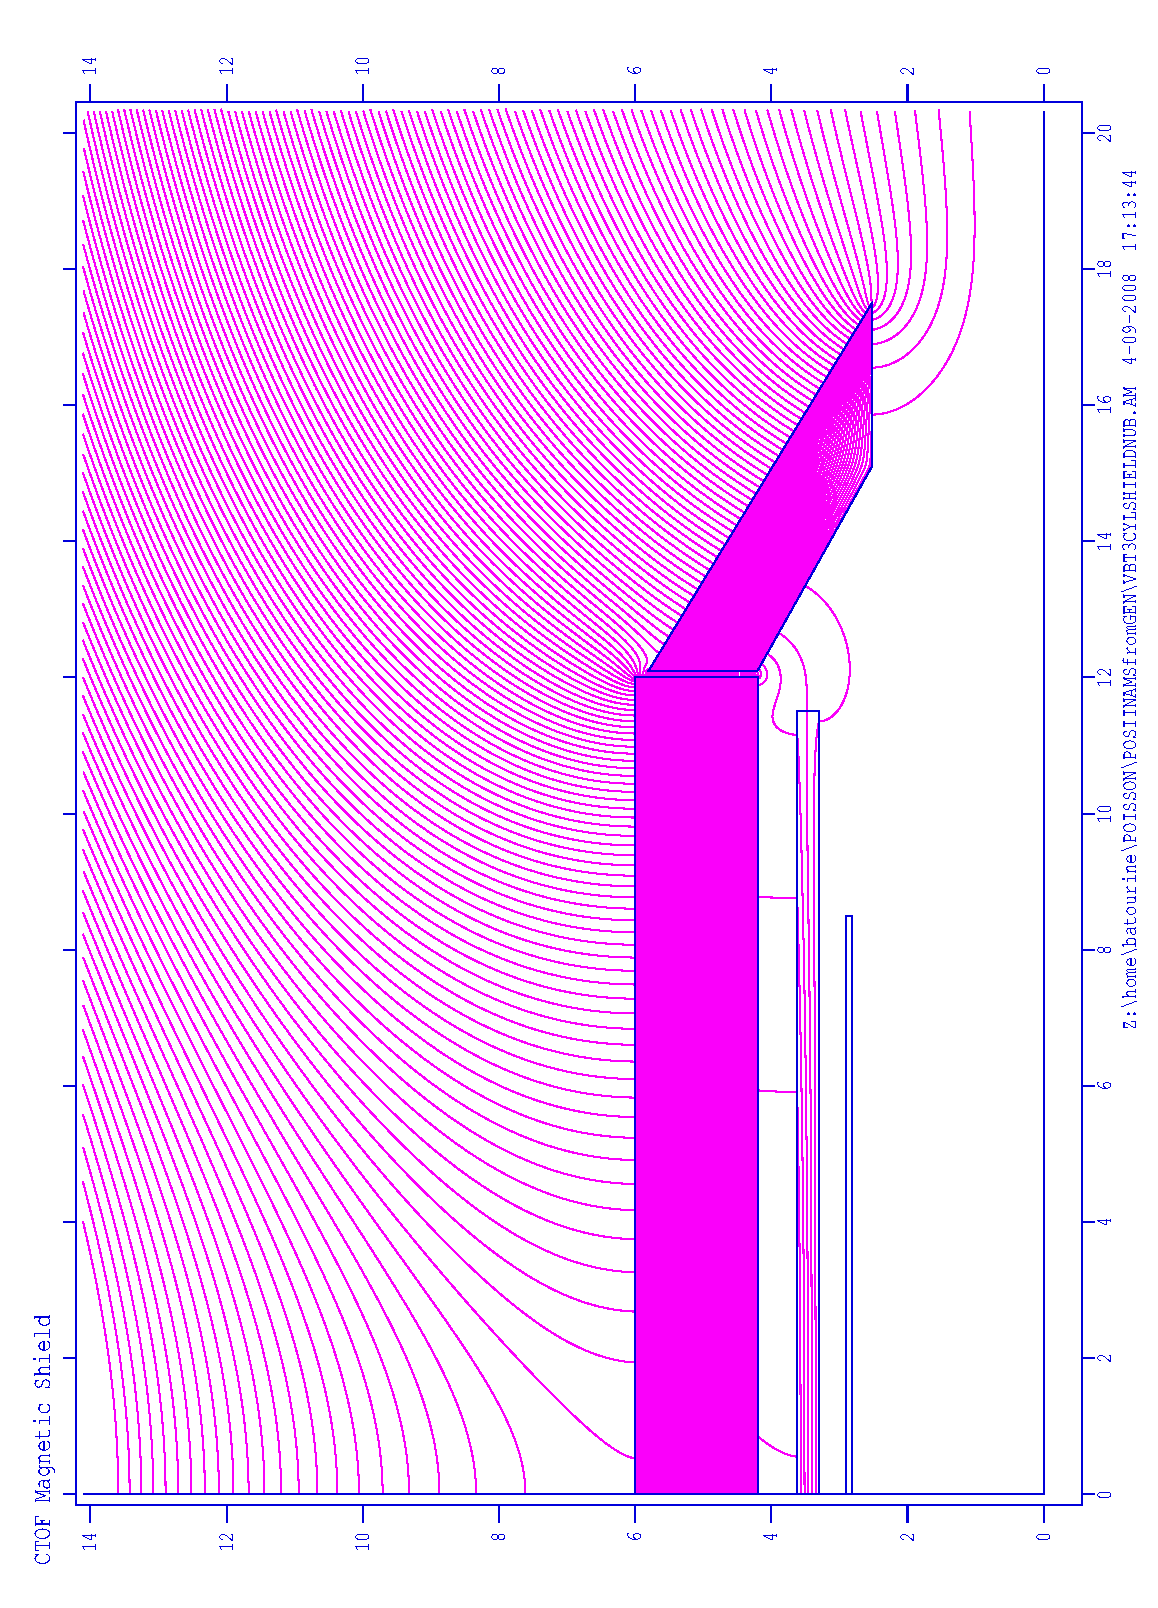
\includegraphics[width=.6\textwidth]{VBT3CYLSHIELDNUB02.eps}
\caption{\small{Sample of a field map for the 3-layer PMT shield in the 
1000~G external field.  The field in the center is 0.5~G.}}
\label{VBT3CYFM}
\end{figure}
%%%%%%%%%%%%%%%%%%%%%%%%%%%%%%%%%%%%%%%%%%%%%%%%%%%%%%%%%%%%%%%%%%%%%%%%%%%

\subsubsection{Hybrid Magnetic Shield with Compensating Coil}

The inner magnetic field strongly depends on the ferromagnetic properties, which 
are very sensitive to the fabrication technology.  Therefore, we are looking for 
more robust protection of the PMTs.  For this purpose, we can consider use of a   
combination of passive and active elements of shielding.  In Fig.~\ref{VBT3CYUS1} 
we present the novel design of a magnetic shield with a compensating coil inside the 
shield assembly.  A small current on the order of 0.1~A running through a 1-mm thick 
wire, is enough to reduce the inner PMT field to the desired values below 0.1~G.
The detailed magnetic field map inside the PMT is shown in Fig.~\ref{VBT3CYUS2}.
As seen from this figure, the internal field is below 0.1~G, while the external field 
is 400~G.

The total current running through the compensating coil is  $\approx$50~A, while the 
coil is $\approx$200-mm long.  Thus it may contain 200 turns of 1-mm thick wire with 
a current of only 0.25~A.  Certainly, higher fields may be exterminated with a higher 
currents in the compensation coil.  Thus, hybrid magnetic shields are very promising. 
We plan further developments and prototyping of this type of shielding.

%%%%%%%%%%%%%%%%%%%%%%%%%%%%%%%%%%%%%%%%%%%%%%%%%%%%%%%%%%%%%%%%%%%%%%%%%%%
\begin{figure}[htbp]
\centering
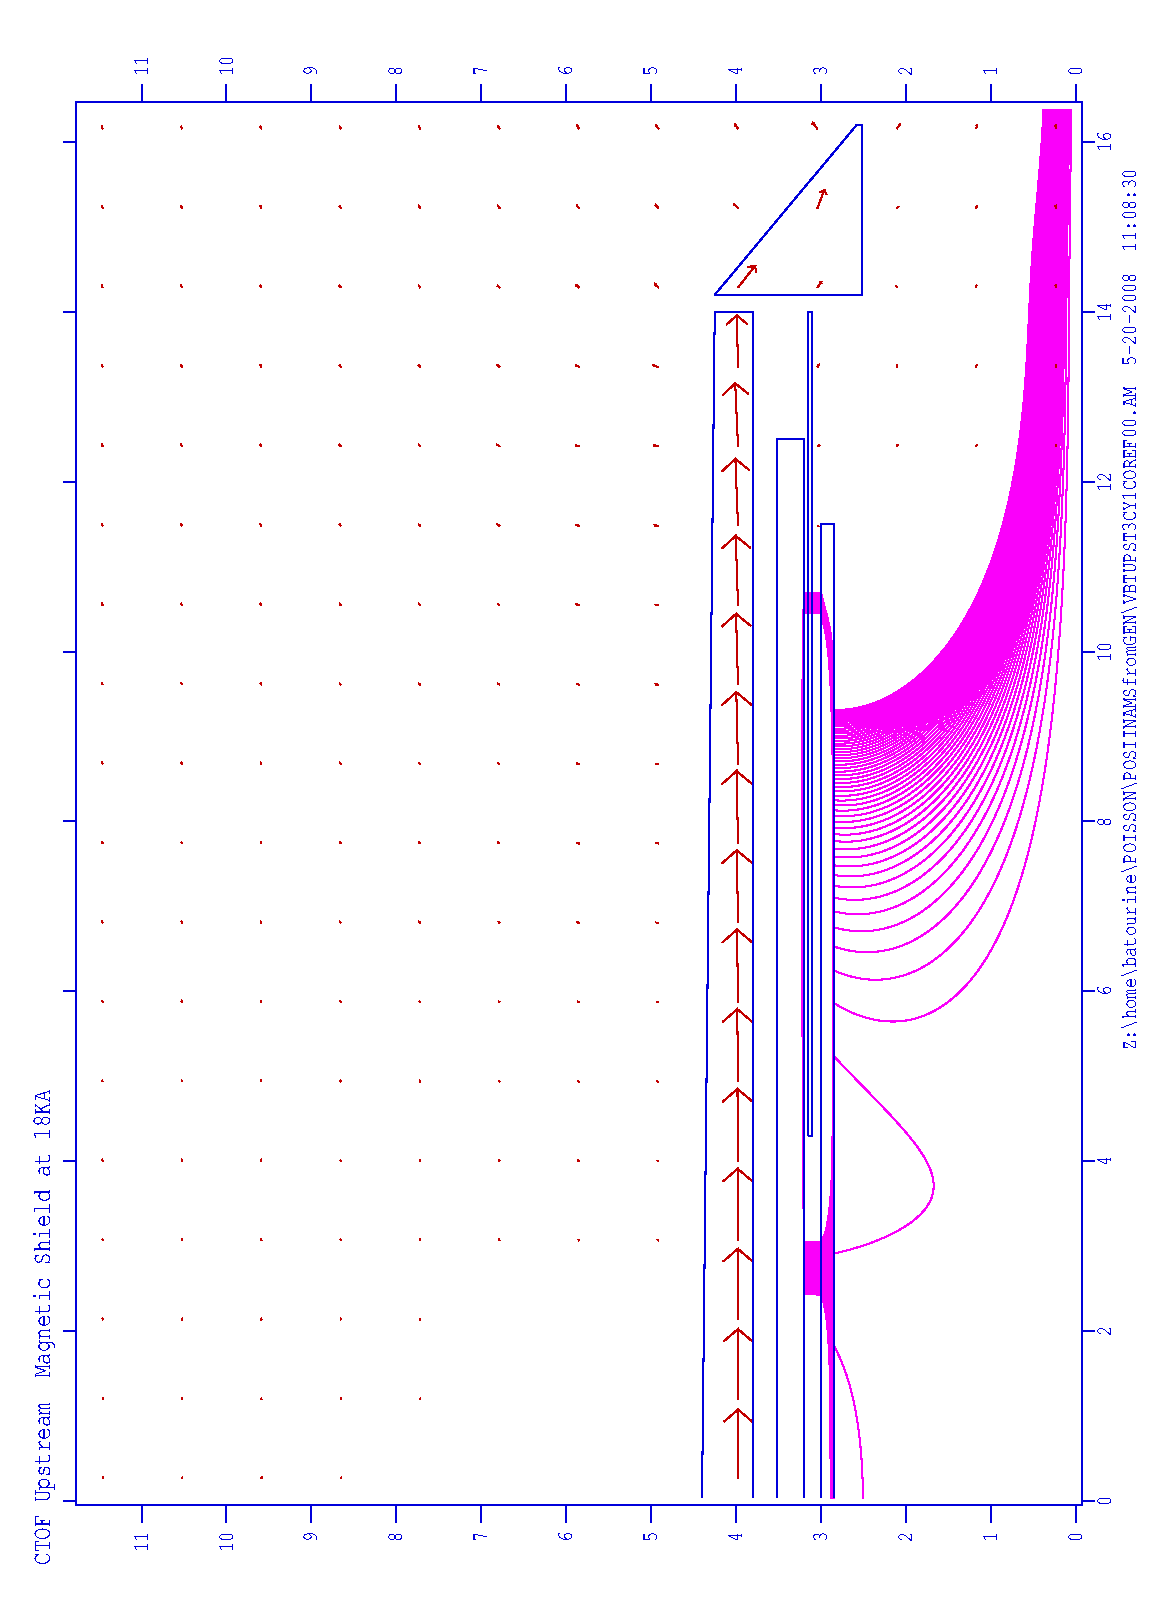
\includegraphics[width=.6\textwidth]{VBTUPST3CY1COREF0001.eps}
%\includegraphics[width=.6\textwidth]{HyMagSh400G.eps}
\caption{\small{Hybrid magnetic shield for the R2083 PMT with the compensating coil
wound around the H2431 assembly.  At in the 400~G external field, the inner PMT field  
is below 0.1~G.}}
\label{VBT3CYUS1}
\end{figure}
%%%%%%%%%%%%%%%%%%%%%%%%%%%%%%%%%%%%%%%%%%%%%%%%%%%%%%%%%%%%%%%%%%%%%%%%%%%

%%%%%%%%%%%%%%%%%%%%%%%%%%%%%%%%%%%%%%%%%%%%%%%%%%%%%%%%%%%%%%%%%%%%%%%%%%%
\begin{figure}[htbp]
\centering
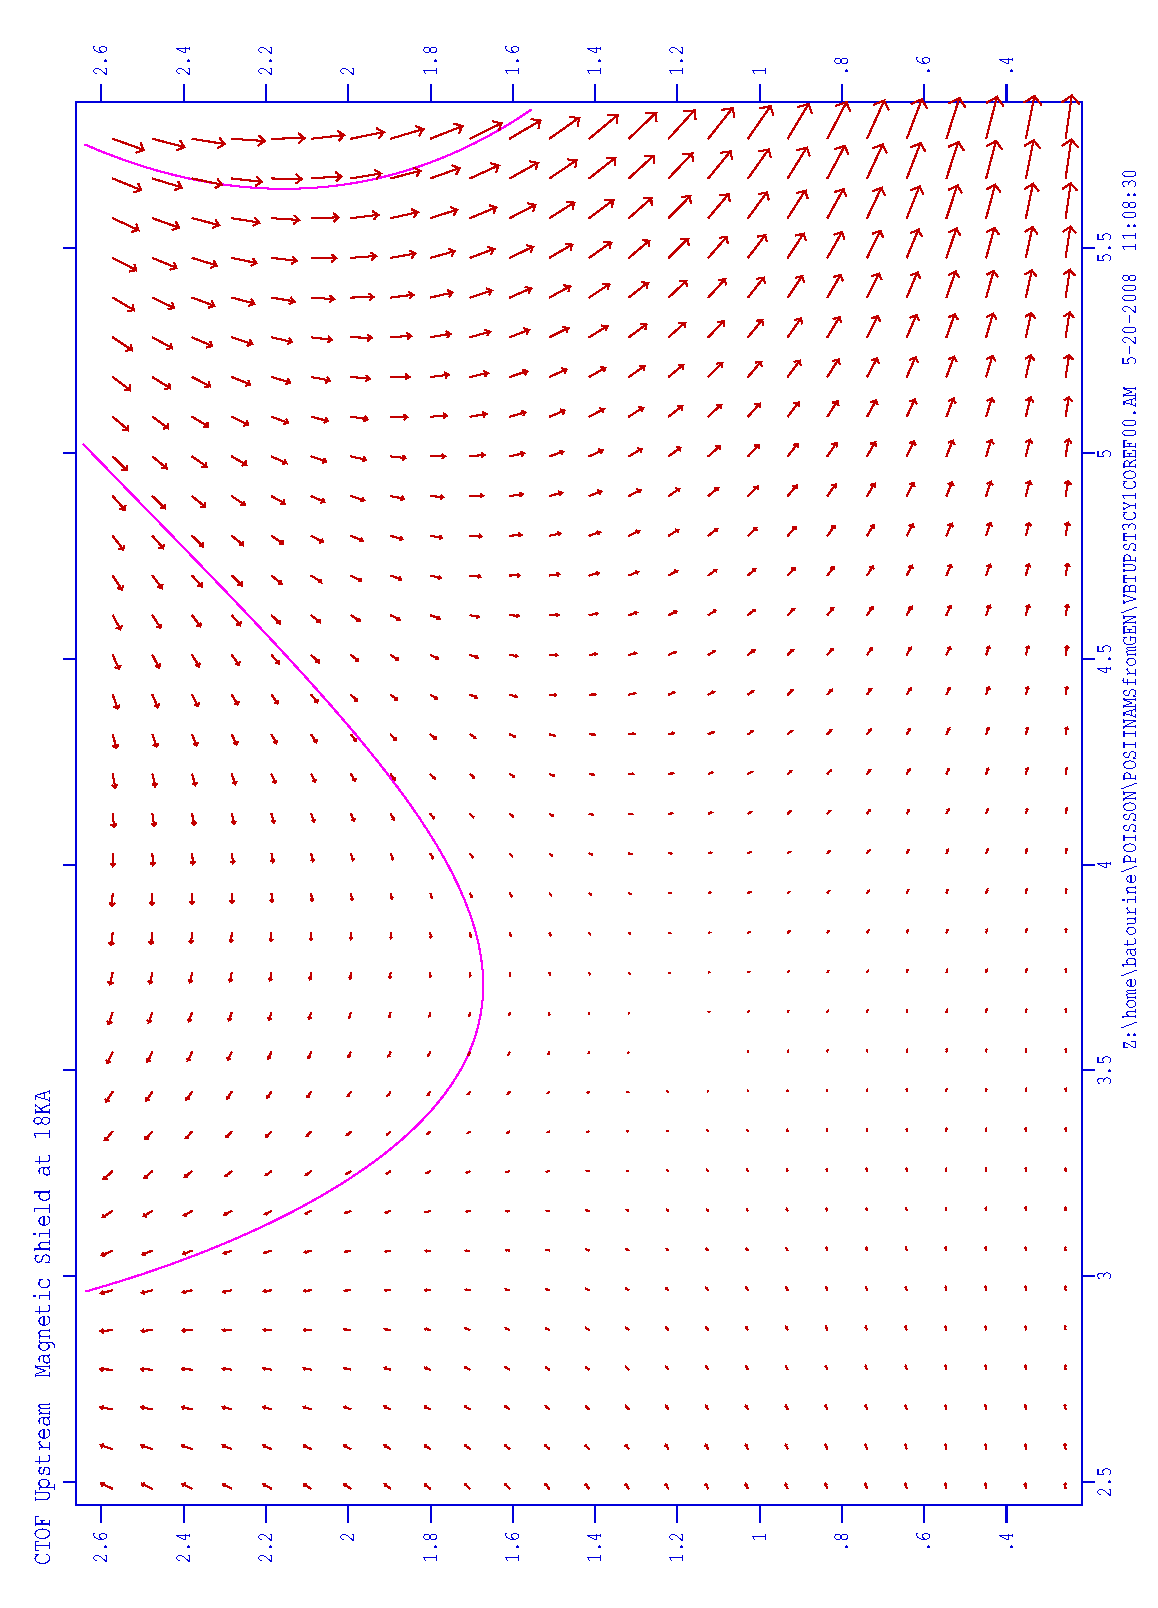
\includegraphics[width=.6\textwidth]{VBTUPST3CY1COREF0002.eps}
\caption{\small{Hybrid magnetic shield for the R2083 PMT with the compensating 
solenoid around the H2431 assembly in a 400~G external field. ``Zoomed in'' field 
map inside the PMT.  The length of arrows indicate the magnetic field.  The maximum 
field, corresponding to the longest arrow, is 1~G.  As seen from this figure, in the 
region of the PMT photocathode at an axial coordinate of $\approx$4~cm, the field is 
0.1~G.}}
\label{VBT3CYUS2}
\end{figure}
%%%%%%%%%%%%%%%%%%%%%%%%%%%%%%%%%%%%%%%%%%%%%%%%%%%%%%%%%%%%%%%%%%%%%%%%%%%

\section{Optical Tests of Acrylic}
  
In our studies of Acrylic light guides~\cite{r1,llg}, we have almost doubled 
the transmittance of our 1-m-long Acrylic light guides, fashioning it as a 
pyramid at the scintillator side and as a cylinder at the PMT end.  In order 
to achieve the desired  $\sigma_{TOF}\approx 50$~ps, a further $\approx$50\%  
improvement of the light guide transmittance is necessary.  Since the light 
guide geometry is almost optimized, a sensible gain may be achieved via modest  
improvement of several factors, e.g. we need shorter and more transparent 
Acrylic with better surface properties, more reflective wrapping, and better 
coupling to the PMTs. 

First we concentrated on the optical properties of commercial cast Acrylic 
rods, which are of special interest for use as our light guides.  Our primary 
motivation was a confusion with manufacturer's specifications for the Acrylic 
transparency.  In their reference measurements, the transparency (92\%--94\%) 
has been determined as a percentage of the radiance passed through a $\approx$3-mm 
thick Acrylic film.  Thus surface reflections are included into the specified 
numbers, which appears to be almost irrelevant to the bulk attenuation. 
Otherwise, the attenuation length would be unrealistically low.  Moreover, a 
better reflection from surfaces is an advantage for light guiding.  Hence, using 
the manufacturer's specifications, one may even neglect what could be a good 
guiding material. 

With this purpose, we have developed simple hand-held tools and methods for 
the express evaluation of Acrylic optical properties.  Such methods are very 
desirable for the detector quality assurance during development and construction.  
We briefly describe these methods in the following sections.

\subsection{Practical Transmittance Measurements}
\label{PTM}

We define the practical transmittance of Acrylic light guides as the ratio of 
the light guide output radiation to the input radiation.  These values are 
the main subject of our efforts, and therefore, we need to measure it quickly 
and precisely, with an accuracy of $\approx$1\%.  This allows us to monitor 
all steps of development and fabrication.
 
%%%%%%%%%%%%%%%%%%%%%%%%%%%%%%%%%%%%%%%%%%%%%%%%%%%%%%%%%%%%%%%%%%%%%%%%%%%
\begin{figure}[htbp]
\begin{center}
\includegraphics[clip=true,angle=-90,width=0.7\textwidth]{LGTEMEASUREMENT.ps}
\end{center}
\caption{\small{Transmittance measurements. (1) Acrylic rod, (2) light source,
(3) Acrylic piece, (4) silicon photodetector, (5) Teflon film as a diffuser, 
(6) mount units, and (7) digital voltmeter.}}
\label{pratra}
\end{figure}
%%%%%%%%%%%%%%%%%%%%%%%%%%%%%%%%%%%%%%%%%%%%%%%%%%%%%%%%%%%%%%%%%%%%%%%%%%%

We measure the practical transmittance in the following way (see Fig.~\ref{pratra}).
Diffuse light is injected into the Acrylic rod (light guide) along its axis from 
one side.  At the opposite end we mount a IL1400 radiometer, which functions as a 
photodetector.  In order to determine the transmittance $T$ we compare two 
measurements of the transmitted radiation $R$.  The first value has been measured  
with a very short reference rod and the second value has been measured with a long 
Acrylic rod.  The difference between the two measurements is due to the transmittance 
of the Acrylic light guide.  This has been estimated as:  

\begin{equation}
T = \frac{R(l_x)}{R(l_s)},
\label{trans}
\end{equation}

\noindent
where $l_x$ is the length of the long rod under test (141.5~cm), $l_s$ is the length 
of the short rod (2.52~cm), and $R(l)$ is the radiation measured with a sample of
length $l$.  We also determine a more ``practical'' attenuation length $\lambda_p$ 
using:

\begin{equation}
\lambda_p= \frac{(l_s-l_x)}{ln(T)},
\label{pracat}
\end{equation}

\noindent
assuming an exponential attenuation along the light guide.
 
For monitoring the luminosity we have developed a method based on precise 
measurements of the consuming power.  For this purpose we record the voltage 
and current of the light source power supply.  We observe a strong correlation 
between the precise voltage and the radiometer's readout.  This correlation has 
been used to bring it to the same voltage, thus to the same radiation power. 

In our first tests, the surface of the Acrylic rod remained as it was processed  
at the factory.  We then had it polished and remeasured the transmittance.
A sample of the measured radiance vs. voltage is shown in Fig.~\ref{leds8}.

%%%%%%%%%%%%%%%%%%%%%%%%%%%%%%%%%%%%%%%%%%%%%%%%%%%%%%%%%%%%%%%%%%%%%%%%%%%
\begin{figure}[htbp]
\begin{center}
\includegraphics[width=13.8cm,clip=true,bb=20 150 620  720]{8ledsalmir2fil071107_picture.ps.gz}
\end{center}
\caption{\small{Practical transmittance measurements.  Top panel: radiance 
of short reference sample.  Bottom panel: radiance of the Acrylic rod under test.
Vertical axis: radiometer readout.  Horizontal axis: power supply voltage ($V$).}}
\label{leds8}
\end{figure}
%%%%%%%%%%%%%%%%%%%%%%%%%%%%%%%%%%%%%%%%%%%%%%%%%%%%%%%%%%%%%%%%%%%%%%%%%%%

From this figure we conclude that the practical transmittance of this Acrylic 
rod is 55.6\%.  In order to test the reproducibility, we repeated measurements 
a second time and measured 58.8\%.   After changing to a stabilized power
supply for the lamp, we measured 58.9\%.  Thus, we have approached the desired 
$\approx$1\% level of accuracy in the transmittance measurement.  Note that
re-polishing the Acrylic rod at the JLab mechanical shop resulted in slightly 
reduced transmittance of 54.4\%.
  
\subsection{Bulk Attenuation Length and Surface Quality}
\label{BAL}

We assume that attenuation of light in the bulk Acylic rod is proportional to 
the inhomogeneity and foreign inclusions.  That is the reason for a luminous line 
in the bulk Acylic irradiated with a strong laser beam ($\approx$1~W).  Therefore, 
we assume that one can estimate the light attenuation length via precise measurement 
of the luminosity of this line.  

\subsubsection{Absolute Measurements}
\label{absmea}

With a narrow laser beam one can determine the absolute value of the bulk 
attenuation length.  The setup and method is similar to that shown in 
Fig.~\ref{pratra}.  As in the former method, we compare two successive 
measurements performed with short and long samples, respectively. The only 
difference is that the laser beam is now axial.  However, the sensitive area 
of the IL1400 photodetector (1$\times$1~cm$^2$) is wide enough to cover the 
transmitted beam, which is just slightly wider than the original beam at the 
same distance.  The bulk attenuation length was then determined using  
Eq.(\ref{pracat}).  The obtained values for various setups and monitoring 
methods are listed in Table~\ref{attlen}.

%%%%%%%%%%%%%%%%%%%%%%%%%%%%%%%%%%%%%%%%%%%%%%%%%%%%%%%%%%%%%%%%%%%%%%%%%%%
\begin{table}[htbp]
\begin{center}
\begin{tabular}{|l|c|c|c|} \hline
Light (nm) & Power Supply & Monitor & $\lambda$ (m) \\ \hline
Laser 475  & $\approx$3 V & light   & $5.4\pm0.7$ \\ \hline
Laser 532  & $\approx$3 V & light   & $5.5\pm0.7$ \\ \hline
Laser 532  & 3.0 V        & current & $6.7\pm0.2$ \\ \hline
Laser 532  & 3.0 V        & current & $6.6\pm0.2$ \\ \hline
\end{tabular}
\end{center}
\caption{\small{Bulk attenuation length ($\lambda$) of the reference 
Acrylic rod.}}
\label{attlen}
\end{table}
%%%%%%%%%%%%%%%%%%%%%%%%%%%%%%%%%%%%%%%%%%%%%%%%%%%%%%%%%%%%%%%%%%%%%%%%%%%

We have convinced ourselves that the measurements with a monitored voltage
(current) of the power supply are more reliable than monitoring of the laser  
luminosity.  Therefore, we determine the bulk attenuation length of the 
Acylic rods from our manufacturer as $\approx 6.65\pm0.5$~m, from the last 
two lines of Table~\ref{attlen}.

\subsection{Relative Measurements}

We have developed a simple express method for relative measurements of  
attenuation in Acylic rods.  For this purpose we detect the light scattered 
at large angles from the area exposed to the laser beam.  A special hand-held  
tool provides a certain acceptance for the radiometer.  The laser beam creates 
a luminous line across the rod.  The radiometer reads the light scattered in 
transverse directions; the surface is excluded from the acceptance.  We have 
checked 2-in rods from several distributors.  The results are listed in 
Table~\ref{samatt}.

%%%%%%%%%%%%%%%%%%%%%%%%%%%%%%%%%%%%%%%%%%%%%%%%%%%%%%%%%%%%%%%%%%%%%%%%%%%
\begin{table}[htbp]
\begin{center}
\begin{tabular}{|l|c|c|r|r|} \hline
 Purchased     & Technology  & Comment,        & Radiance    & $\lambda(m)$ \\
    from       &             &  status         & (nW/cm$^2$) &              \\ \hline
Prof. Plastic-0& cast,1.41 m & reference       & 17.7        & $6.65\pm0.2$  \\ \hline
Plast. Craft-1 & cast,148 mm & pol. butt-ends  & 16.1        & $7.31\pm0.3$ \\ \hline
Plast. Craft-2 & cast,153 mm &unpol.butt-ends  & 21.6        & $5.44\pm0.3$ \\ \hline
Plast. Craft-3 & cast,200 mm &unpol.butt-ends  & 32.1        & $3.66\pm0.2$ \\ \hline
KNU sample     & cast,205 mm & pol. butt-ends  & $\ge18.2$   & $\leq 6.1$    \\ \hline  
McMaster-Carr Supp.Cmp.& extr.,400 mm & unpol. butt-ends & 48.7 & $2.42\pm0.2$ \\ \hline
\end{tabular}
\end{center}
\caption{\small{Bulk attenuation length ($\lambda$ (532 nm)) of 2-in Acrylic 
rods from different manufacturers.}}
\label{samatt}
\end{table}
%%%%%%%%%%%%%%%%%%%%%%%%%%%%%%%%%%%%%%%%%%%%%%%%%%%%%%%%%%%%%%%%%%%%%%%%%%%

The dispersal of the radiometer readout is significant.  These values are 
calibrated in units of attenuation length, as was described in the previous 
section.  The samples vary in attenuation length\footnote{The readout values 
are calibrated in units of attenuation length as described in Section~\ref{absmea}.} 
by almost a factor of three.  The 2-in Acylic rods from Professional Plastic Inc.
gives $\approx$18~nW/cm$^2$ in our hand-held tool.  This value will be our future 
reference.  The best readout (over the length) for the Acylic sample from South 
Korea is about the same.  However, this sample has numerous local inclusions 
separated by a few mm.  These inclusions manifest themselves as a reduced 
practical transmittance ($\lambda_p \approx$1.5-2~m) of the sample.  In addition, 
due to the fact that this rod was machined (with a lathe) from a flat piece of  
Acylic, its surface was damaged, perhaps to the depth of a few microns, which 
resulted in a hazy view from the end of the rod.    

We have selected Professional Plastic Inc. as our provider of Acylic for the 
{\tt CTOF} project.  However, we plan further casting for better Acylic samples.

\subsection{Surface Quality Measurements}

We have developed an express method for estimating the quality of a polished surface.  
This method is based on measuring the scattered light from the light guide surface 
illuminated with a laser beam.  A special hand-held tool provides a certain surface 
impact angle and acceptance for the IL1400 radiometer.   Note that in this case some 
part of the bulk scattered light is also accepted by the radiometer.  However, it may 
be subtracted from the readout.  The method has been calibrated with the reference 
Acrylic rod.  The typical reference readout of the IL1400 with this rod was 
20~nW/cm$^2$.  

\paragraph{Practical Transmittance After Polishing:}
Unfortunately, after we had the JLab mechanical shop polish our Acrylic samples, 
the surface readout increased by 50\%.  The scratches on the polished surface
indicate that this problem was caused by the environment in the shop.

\paragraph{Practical Transmittance After Painting with Lacquer:}
The technique of vapor polishing is very close to painting.  Therefore, we have 
checked the effect of painting on the practical transmittance of a previously 
buffed 20-cm long Acylic rod.  The result is quite confusing.  The surface readout 
dropped almost by a factor of two after painting with Acylic lacquer.  The 
surface looks quite smooth.  However, the practical transmittance of a 205-mm long 
sample dropped by $\approx$10\%.  The possible reasons for this unexpected effect  
are firstly, the higher refractive index, secondly, surface cracks due to aggressive 
solvents, and thirdly, worse transmission spectrum of the laser.  All of this
has to be carefully investigated in future.

\subsection{Future Applications}
\label{CAO}

We have developed express hand-held methods for measuring both the bulk and the 
surface attenuation of light guides.  Our basic assumption on the proportionality 
of the attenuation to the scattering has to be verified.  The developed methods 
allow us the following:

\begin{itemize}
\item to assure a proper attenuation length of Acylic in the light guides;
\item to monitor the surface quality of light guides;
\item to perform R\&D for better light guide transmittance.
\end{itemize} 

The immediate practical results of these methods include:

\begin{itemize}
\item we have selected the manufacturer of Acylic rods with the lowest attenuation;
\item customer buffing does not necessarily improve the surface quality; other 
methods should be used;
\item manufacturer's specifications should be interpreted with care.
\end{itemize}

We plan to use these methods for comparison of Acylic surfaces after  
ordinary buffing, flame polishing, and, perhaps, vapor polishing.

\section{Studies with Monte Carlo Calculations}
\label{mutchler}

We have calculated the transport efficiency of the light guides using the 
code BARTIM described in the Appendix of Ref.~\cite{mutch}.  In this 
Monte Carlo program, a photon is either totally internally reflected or 
reflected or refracted according to the Fresnel equations.  Imperfections 
on the surface are modeled by reducing the total internal reflection 
co-efficient, IR, below 100\%.  The light that escapes the scintillator (or 
light guide) is specularly reflected with the appropriate reflection 
co-efficient $R$.  The calculations were performed for the light guide 
configuration shown in Fig.~\ref{bentlg03}.  The dimensions given in 
Figs.~\ref{lgupstream} and \ref{lgdownstream} for the upstream and downstream 
light guides, respectively, were used.  The beam was taken to be incident 
normally at the center of the scintillator.  The transmission and loss of 
light at various positions are tabulated in Table~\ref{mud1}.

%%%%%%%%%%%%%%%%%%%%%%%%%%%%%%%%%%%%%%%%%%%%%%%%%%%%%%%%%%%%%%%%%%%%%%%%%%%
\begin{table} [htbp]
\begin{center}
\begin{tabular}{|l|c|c|} \hline
Percentage lost at a given position  & Upstream & Downstream \\ \hline
Scintillator - light guide interface & 5.9      & 16.9       \\ \hline 
Absorption (all sections)            & 20.7	& 16.8 	     \\ \hline
Lost in straight sections  	     & 25.0	& 17.6 	     \\ \hline
Lost in bends  	                     & --	& 10.2       \\ \hline
Lost at PMT  	                     & 3.8 	& 2.9        \\ \hline \hline 
Transmitted  	                     & 44.6	& 35.5 	     \\ \hline
\end{tabular}
\caption{\small{Calculated values of the light guide transmission efficiency 
and losses for the two sides.}}
\label{mud1}
\end{center}
\end{table}
%%%%%%%%%%%%%%%%%%%%%%%%%%%%%%%%%%%%%%%%%%%%%%%%%%%%%%%%%%%%%%%%%%%%%%%%%%%

The parameters used in this calculation were $R$=0.9, IR=0.99, and a bulk 
attenuation length of 4~m in the Acrylic.  It was assumed that the wrapping 
was a radiant mirror film VM-2000 from 3M as described and measured in 
Ref.~\cite{mutch}.

\subsection{Effect of Trapezoidal Shape of Scintillator on Light Propagation}
\label{mu1}

The effect of the scintillator's trapezoidal cross section was investigated.  
It was found that only about 7.2\% of the light generated in the center of the 
scintillator was lost, compared with a rectangular scintillator bar.  The 
sloped sides of the light guide, that allowed the 46-mm cylinder to mesh with 
the smaller scintillator, may actually improve the light transport efficiency. 
It directs the light upward, which is needed to match the direction of the 
light guide. 

\subsection{Effect of Coupling Angles Between Light Guides and Scintillators}
\label{mu2}

The effect of changing the pitch angle of the upstream light guide from 
18$^\circ$ to 30$^\circ$ was investigated.  The transmission varied by less 
than 1\%.  Varying the downstream angle is more difficult as it would impinge 
on the forward acceptance.  Therefore we did not investigate this.

\subsection{Effect of Bending}
\label{mu3}

The effect of varying the bend radius of the upstream light guide was examined.
The radius was varied from 10.0, 11.75, 13.3 to 14.3~cm.  Surprisingly, the 
results were insensitive to the radius of the bend.  The smaller the radius, 
the smaller the losses in the bend, but this was compensated for by increased 
losses in the straight sections, which were now longer.  This seems 
counterintuitive, but the bend radius appears to be sufficiently large that the 
losses are dominated by the length of a given section.  

\subsection{Effect of Up and Down Mirrors of Light Guides}
\label{mu4}

The effect of the angle and the quality of the polish, IR value, are shown in 
the top and bottom panels of Fig.~\ref{trans1}.  There is a weak dependence on 
the lower angle, with a broad maximum at about 9$^\circ$.  This angle was used 
in the calculations shown in Table~\ref{mud1}.  The dependence on the upper 
angle is even weaker.  We took it to be 9$^\circ$ also, but any angle between 
7$^\circ$ and 15$^\circ$ is acceptable. 

%%%%%%%%%%%%%%%%%%%%%%%%%%%%%%%%%%%%%%%%%%%%%%%%%%%%%%%%%%%%%%%%%%%%%%%%%%%
\begin{figure}[htbp]
\centering
\includegraphics[width=0.7\textwidth]{trans.ps}
\caption{\small{Light transmission vs. 1). the ``down mirror'' orientation 
angle (left panel) and 2). the reflectivity of the light guide surface (right 
panel).}}
\label{trans1}
\end{figure}
%%%%%%%%%%%%%%%%%%%%%%%%%%%%%%%%%%%%%%%%%%%%%%%%%%%%%%%%%%%%%%%%%%%%%%%%%%%

\subsection{Light Guide Transmission Efficiency vs. Refractive Index}
\label{mu5}

We compared the light guide transmission efficiency for two materials -- 
Acrylic ($n$=1.49) and Lexan ($n$=1.58) -- to estimate the benefit of using
a more optically dense material for the light guides.  If we assume equal 
attenuation lengths, Lexan transmits 10\% more light, primarily by 
eliminating the losses at the scintillator -- light guide interface. 
Unfortunately the transparency of Lexan is about half that of Acrylic.
Taking this into account, the Lexan transmits only 93\% of the light. 
However, we have to consider this option, keeping in mind possible  
progress in the plastic industry.

\subsection{Matching of the Light Guide to the PMT Entrance Window}
\label{mu6}

The photocathode of the R2083 PMT is $\approx$1-mm thick in the center.  
According to the information obtained from the Hamamatsu experts, the 
shape of the photocathode is a sphere of 55~mm in radius with 
$\approx \pm 25^\circ$ polar opening.  On the other hand, the entrance 
window is flat.  Therefore, the distance between the flat end of the light 
guide and the photocathode ranges from 1~mm in the center to 6~mm at the 
edge of the photocathode.  That may cause significant loss of light through 
the edges of the PMT entrance window.  If the scintillator is directly 
coupled to the PMT, 32\% of the light output is lost.  However after the 
light has been transported through the light guide, the phase space has 
been restricted to mostly forward angles. In this case the loss is only 8-9\%.

\subsection{Effect of the Photocathode Diameter}
\label{mu7}

The number of reflections drops if the light guide has a larger diameter in 
its cylindrical part.  The downstream light guide was modeled with a 52.0-mm 
diameter light guide.  This transported about 6\% more light to the PMT, but 
it was then lost.  A larger diameter tube could collect most of this light, 
giving a net gain in the signal.

Another possibility that we have investigated is the use of a reducing cone 
at the end coupled to the PMT.  The length of the cone was varied, keeping 
the overall length of the cone plus the last straight section constant at 
250~mm.  In accordance with Fig.~\ref{plgef}, the optimum length of the cone 
was found to be about 50~mm.  However this did not improve the light guide 
transmission.  Once again the extra light was lost at the PMT. (Note, the 
effect of the curvature of the photocathode was taken into account in these 
calculations).

\subsection{Effect of Light Guide Length}
\label{mu8}

We investigated the effect of decreasing the light guide length by about 
250~mm.  This yields a transport efficiency of 48.8\% for the upstream 
light guide and 37.8\% for the downstream light guide.  This is an 
$\approx$10\% and 6\% improvement over the numbers quoted in Table~\ref{mud1} 
for 1-m long light guides, respectively.  This result may be used for further 
estimations of longer light guides.

\subsection{Light Guides to Metal-Channel Photomultipliers}
\label{mu9}

Finally, we investigated the possibility of using rectangular Hamamatsu 
metal-channel tubes with shorter light guides.  If a tandem of such PMTs  
and on-board preamplifiers can tolerate magnetic fields up to $\approx$0.3~T, 
then it may be placed closer to the scintillator.

A tube that might be suitable is the Hamamatsu H8500 that has a photocathode 
$49\times49$~mm$^2$.  The minimum light guide length is constrained by the 
requirement that the tubes ($52\times52$~mm$^2$ external size) are at a radius 
sufficient to provide clearance between the tubes.  This would be about 
70~cm for the upstream light guide and 50~cm for the downstream one.

For preliminary estimations the light guides were taken to be straight guides 
40-mm wide by 47.5-mm thick.  The transmission and loss of light at various 
positions are tabulated in Table~\ref{mud2}.  The loss at the PMT was not 
estimated since the light guide is smaller than the photocathode and the 
photocathode is flat.

%%%%%%%%%%%%%%%%%%%%%%%%%%%%%%%%%%%%%%%%%%%%%%%%%%%%%%%%%%%%%%%%%%%%%%%%%%%
\begin{table} [htbp]
\begin{center}
\begin{tabular}{|l|c|c|} \hline
Percentage lost at a given position  & Upstream & Downstream \\ \hline
Scintillator - light guide interface & 5.9      & 16.9       \\ \hline 
Absorption                           & 15.9	& 10.4 	     \\ \hline
Lost from sides  	             & 19.9 	& 16.0 	     \\ \hline
Lost at PMT  	                     & N/A 	& N/A 	     \\ \hline \hline 
Transmitted  	                     & 58.3 	& 56.7 	     \\ \hline
\end{tabular}
\end{center}
\caption{\small{Calculated values of the light guide transmission efficiency 
and losses for rectangular light guides.  The upstream side guide is 70-cm 
long angled at 22$^\circ$ and the downstream guide is 50-cm long angled at 
45$^\circ$.  There are no other bends in the light guides.  The light guides 
are coupled to rectangular Hamamatsu H8500 tubes $49\times 49$~mm$^2$.  The 
light guides are 40-mm wide and 47.5-mm thick.}}
\label{mud2}
\end{table}
%%%%%%%%%%%%%%%%%%%%%%%%%%%%%%%%%%%%%%%%%%%%%%%%%%%%%%%%%%%%%%%%%%%%%%%%%%%

This is a 30\% and 58\% increase in the light transmission efficiency, 
respectively, over the results in Table~\ref{mud1}.  However these gains 
will be offset by the reduced photocathode efficiency of a metal-channel 
tube, which is typically 20--22\% vs. the 26--28\% of regular tubes.  However, 
there will be a net gain on the downstream side and the pulse height on the 
two ends will be approximately equal. 

\section{Estimations of $\sigma_{TOF}$ for Different CTOF Designs}
\label{estimates}

According to Table~\ref{mud1}, the light transport efficiency of an optimized 
straight light guide is $LTE$=44.6\%.  This value is in agreement with the 
previous experimentally determined value $44.2 \pm 4$\%.  The $LTE$ of the 
bent light guide is lower, 35.5\% (see Table~\ref{mud1}).

Using the previously measured $\sigma_{PMT}$=77.9~ps (see Table~\ref{crt}), 
obtained with a symmetric counter and 1-m long straight ``pyramid'' light 
guides, we can estimate the time-of-flight resolution of optimized 
asymmetric counters in the following way.  As was shown in Ref.~\cite{r4} 
for asymmetric light collection, the best timing is achieved by using a 
weighted average of the two PMTs with $\sigma_A$ and $\sigma_B$ respectively:

\begin{equation}
\label{eq0}
\sigma_{TOF}=\sqrt{\frac{(A\sigma_A)^2+(B\sigma_B)^2}{(A+B)^2}},
\end{equation}

\noindent
where $A$ and $B$ are proportional to the pulse heights (amount of light) 
of the two tubes, attached to straight ($A$) and bent ($B$) light guides, 
respectively.  Note that $A \propto LTE_A$, as well as  $B \propto LTE_B$.
If we define $f = A/B$ and $\sigma_{PMT}=\sigma_A= \frac{1}{\sqrt{f}}\sigma_B$,
then

\begin{equation}
\label{eq1}
\sigma_{TOF}=\sigma_{PMT}\sqrt{\frac{f}{1+f}}.
\end{equation}

\paragraph{Resolution with 1-m Long Light Guides:}

Using data from Table~\ref{mud1} we find:  

\begin{equation}
\label{eq2}
f = \frac{A}{B}=\frac{LTE_A}{LTE_B}=44.6/35.5=1.256.
\end{equation}

\noindent
Thus for an asymmetric counter with 1-m long light guides we estimate:

\begin{equation}
\label{eq3}
\sigma_{TOF} = 0.746\times\sigma_{PMT} = 0.746\times77.9~{\rm ps} =
58.1~{\rm ps},
\end{equation} 

\noindent
which is only 16\% worse of the desired value 50~ps. However, that means 
that the amount of light would have to be increased by a factor of
1.16$^2$=1.346.

\paragraph{Resolution with 1.5-m Long Light Guides:}

If the total length of the light guides is 1.5~m, the amount of light will 
drop by $\approx$22\% (see Ref.~\ref{mu8}), thus the resolution will be 
$\approx$64~ps, which is 28\% worse than the desired value.  In this
regard, we hope that improving the surface quality up to IR-0.995 using  
cast Acylic for the light guides and wrapping them with VM2000, may gain us
a factor of $\approx$1.2 in the number of photons at the PMT window.
Thus we may gain a total factor of $\approx$1.1$^{-1}$ in the resolution, 
i.e. $\sigma_{TOF}\approx$58~ps.  In a pessimistic scenario we may 
simply increase the thickness of the scintillator to 4~cm to get an 
additional factor of $\approx1.15^{-1}$.

\paragraph{Resolution with Metal-Channel PMTs H8500 and Light Guides:}

Below we consider a counter with two H8500 MC PMTs viewing the scintillator 
via light guides $700 \times 40 \times 47$~mm$^3$ and 
$500 \times 40 \times 47$~mm$^3$ in size.  In this estimation we assumed 
that in direct contact to the scintillator the resolution of the H8500 is 
the same as for the R2083.  This is a reasonable assumption since the timing 
characteristics of these PMTs are almost identical.  The estimate was done 
in the same way as above for the R2083 PMT, using the calculated parameters 
of the light guides given in Table~\ref{mud2}.  The resulting estimate for 
$\sigma_{TOF}\approx$49~ps is listed in Table~\ref{table4}, row~5.  Of 
course, we plan to measure the resolution of the H8500 PMT in the environment 
of a high magnetic field.

%%%%%%%%%%%%%%%%%%%%%%%%%%%%%%%%%%%%%%%%%%%%%%%%%%%%%%%%%%%%%%%%%%%%%%%%%%%
\begin{table}[htbp]
\begin{center}
\begin{tabular}{|c|c|c|c|c|c|} \hline
                        &     &               &                      & RF reference      & Light  \\ 
Counter design          & $f$ & $LTE_l/LTE_r$ & $\sqrt\frac{f}{1+f}$ & $\sigma_{TOF}$/ps & deficiency  \\ 
LG $\leftrightarrow$ LG &     &               &                      &                   & factor  \\ \hline
Pyr. $\leftrightarrow$ Pyr. & 1.00 & .44/.44  & 0.71 & \textbf{55}   & 1.21   \\
1~m, 2$\times$ R2083    &     &               &      &  ref. measur. &         \\ \hline
Pyr. $\leftrightarrow \supset$ Pyr.& 1.25     & .446/.355   & 0.75 & 58 &  1.35      \\
1~m, 2$\times$ R2083    &      &     &     &  $estimate$  &           \\ \hline
Pyr. $\leftrightarrow \supset$ Pyr.& 1.19  & .372/.313   & 0.737 & 63 &  1.58      \\
1.5~m, 2$\times$ R2083  &      &     &     &    $estimate$    &           \\ \hline
Bar $\leftrightarrow $ Bar & 1.03 & .583/.567 & 0.712 & 49  & 0.94         \\
0.7~m, 2$\times$ H8500  &      &     &     &   $estimate$   &           \\ \hline
MCP PMT$\leftrightarrow $MCP~PMT & 1. & 1./1. & 0.71& 61 at 1.0~MHz & 1.5 \\
2$\times$ Burle~85011   &      &     &     & 50 at 0.1~MHz  &           \\ \hline
CTOF counter       & 1.33   & .4/.3& 0.76 & 60    & 1.4     \\
(1.4m \& 1.6m)     &       &      &      &    $estimate$     &       \\ \hline
\end{tabular}    
\caption{\small{TOF resolution for different CTOF counter designs.  The 
measured reference values from lines 6, 9, and 10 of Table~\ref{crt} were 
used to evaluate $\sigma_{TOF}$.}}
\label{table4}
\end{center}
\end{table}
%%%%%%%%%%%%%%%%%%%%%%%%%%%%%%%%%%%%%%%%%%%%%%%%%%%%%%%%%%%%%%%%%%%%%%%%%%%

\section{Pilot Design with FM/MC Photomultipliers}

In parallel we will develop the design with PMTs capable of operating in high  
magnetic fields.  In addition to measurements with fine-mesh PMTs, we plan  
to measure the time resolution with metal-channel PMTs.  Unlike fine-mesh 
PMTs, such photo-detectors are sensitive to magnetic fields.  However, the 
signal rise time of metal-channel PMTs is significantly shorter compared to 
fine-mesh PMTs (0.8~ns vs. 2.7~ns).  We plan to test H8500 PMTs, with a magnetic 
shield, up to fields of 0.2~T, most probably with amplification to the PMT signals, 
as was done in our studies with MCP PMTs.

In the low-field area of $\leq$0.3~T, fine-mesh/metal-channel PMTs may be used 
with light guides $\leq$0.8-m long.  In addition, their sensitive surface is 
wider ($49\times49$~mm$^2$), therefore an expanding light guide may deliver 
more light to the photocathodes.  

The pilot design, utilizing advantages of fine-mesh/metal-channel PMTs, is 
shown in Fig.~\ref{JLABt0H8500}.  The scintillators are of the same shape 
as in the design with conventional R2083 PMTs.  The upstream and downstream 
light guides, delivering light to the area of tolerable magnetic fields  
are 86-cm and 50-cm long, respectively, with corresponding pitch angles of  
21$^\circ$ and 45$^\circ$.  These parameters provide room for the 50 adjacent 
H8500 PMTs at $r\approx$55~cm.

%%%%%%%%%%%%%%%%%%%%%%%%%%%%%%%%%%%%%%%%%%%%%%%%%%%%%%%%%%%%%%%%%%%%%%%%%%%
\begin{figure} [htbp]
\centering
\includegraphics[width=0.8\textwidth]{JLABt0H8500.ps}
\caption{\small{The design of the {\tt CLAS12} CTOF counter with H8500 
PMTs from Hamamatsu.  Acrylic light guides may be rectangular in cross 
section at the photocathode ($49\times49$~mm$^2$). The length of the 
upstream/downstream light guides is 863/441~mm, respectively.  At the 
scintillator end, the light guides and the Bicron-408 are trapezoids in 
cross section.  Magnetic fields are shown with vectors.}}
\label{JLABt0H8500}
\end{figure}
%%%%%%%%%%%%%%%%%%%%%%%%%%%%%%%%%%%%%%%%%%%%%%%%%%%%%%%%%%%%%%%%%%%%%%%%%%%

The light guides will be rectangular in cross section at the PMT side for 
the metal-channel H8500 PMTs.  At the scintillator side, they will have a 
trapezoidal cross section of variable size, which couples to the cross section 
of the scintillator at the corresponding end.  Up to a certain radius of 
$\approx$39~cm, the light guides are in close contact to each other, thus 
forming a body enclosed between two cones. Above this radius the light guides 
form a ``fan''.  Similar to the light guides for the R2083 PMT design, they 
have ``focusing mirrors'' at the scintillator side.  These relatively short 
straight scintillators may be easily machined or casted.  The expected 
resolution ($\approx$49~ps) of counters with metal-channel PMTs is listed in 
Table~\ref{table4}.

In the design with fine-mesh PMTs, the light guides may be even shorter.
We plan future resolution tests with fine-mesh PMTs of large sensitive area, 
such as the R5924, instrumented with realistic light guides.

\section{Pilot Design with Micro-Channel Plate PMTs}
\label{des85011}

A general view of the pilot {\tt CLAS12} CTOF counter with 85011 MCP PMTs 
from Burle is shown in Fig.~\ref{JLABt0H85011}.  A detailed view is shown in  
Fig.~\ref{JLABH85011}.  One multi-anode PMT is supposed to convert the light 
from two scintillators, left and right.  

%%%%%%%%%%%%%%%%%%%%%%%%%%%%%%%%%%%%%%%%%%%%%%%%%%%%%%%%%%%%%%%%%%%%%%%%%%%
\begin{figure} [htbp]
\centering
\includegraphics[width=0.75\textwidth]{JLABt0H85011.ps}
\caption{\small{General view of the {\tt CLAS12} CTOF counter with 
Burle 85011 MCP PMTs.  (1) Mirror film, (2) two adjacent scintillators,
and (3) Burle 85011 multi-anode assembly.}}
\label{JLABt0H85011}
\end{figure}
%%%%%%%%%%%%%%%%%%%%%%%%%%%%%%%%%%%%%%%%%%%%%%%%%%%%%%%%%%%%%%%%%%%%%%%%%%%

%%%%%%%%%%%%%%%%%%%%%%%%%%%%%%%%%%%%%%%%%%%%%%%%%%%%%%%%%%%%%%%%%%%%%%%%%%%
\begin{figure} [htbp]
\centering
\includegraphics[width=0.7\textwidth]{JLABH85011.ps}
\caption{\small{A closer view of the {\tt CLAS12} CTOF counter with Burle
85011 MCP PMTs.}}
\label{JLABH85011}
\end{figure}
%%%%%%%%%%%%%%%%%%%%%%%%%%%%%%%%%%%%%%%%%%%%%%%%%%%%%%%%%%%%%%%%%%%%%%%%%%%

The outputs of the corresponding anodes will be assembled to produce a common 
signal for each scintillator.  The scintillators, Bicron-408, are machined 
with a trapezoidal cross section.  We note that the inner radius can be 
reduced in two different ways, provided that the sizes of the PMT housings 
remain the same $(72\times72$~mm$^2$).  The first way is via implementing  
staggered counters, as shown in Fig.~\ref{JLABH85011-1}.  In this case 
$r_{min}$=206~mm, but the length of scintillators has to be increased by 
52~mm (the thickness of the 85011 PMT assembly).  The second option is to 
reduce the number of counters from 50 with $r_{min}$=275~mm to 44 with 
$r_{min}$=250.4~mm.

%%%%%%%%%%%%%%%%%%%%%%%%%%%%%%%%%%%%%%%%%%%%%%%%%%%%%%%%%%%%%%%%%%%%%%%%%%%
\begin{figure} [htbp]
\vspace{7.7cm}
\special{psfile=JLABH85011-1.ps hscale=57 vscale=57 hoffset=10 voffset=0}
\caption{\small{Staggering the CTOF counters with Burle 85011 MCP PMTs.}}
\label{JLABH85011-1}
\end{figure}
%%%%%%%%%%%%%%%%%%%%%%%%%%%%%%%%%%%%%%%%%%%%%%%%%%%%%%%%%%%%%%%%%%%%%%%%%%%

\section{Outlook}

We have experimentally verified that the resolution of our test 
installation is mostly dictated by the statistics of the primary photons.  
We have measured a reference resolution for the setup of three counters with 
long light guides.  With this reference value we have estimated the 
time-of-flight resolution (relative to the RF signal of the accelerator) for 
different counter designs.  Estimations were done using Eq.(\ref{eq0}) and  
Eq.(\ref{eq1}).  The resulting values are listed in Table~\ref{table4} 
together with the deficiency factors in the amount of light.

\paragraph{CTOF Counter with Conventional R2083 PMTs:}

For the current design with 1.3--1.5m long light guides (row-7) the resolution 
is likely to be improved to the desired value with better technology for
the light guide production and further optimization of the design, including 
bent and thicker scintillators ($\approx$4~cm).  The desired increase of 
total transmittance is about 40\%, i.e. the transmittance has to be 50\% 
and 60\% for the downstream and upstream light guides, respectively.

\paragraph{CTOF Counter with MCP PMTs:}

Recently we found a way to form a dense barrel with MCP PMTs from Burle, 
or similar PMTs from Hamamatsu.  The design with MCPs looks promising. 
According to our recent measurements with Burle 85011 PMTs, the timing 
resolution may be as good as 61~ps (see Table~\ref{table4}, row-6 ) at a
1~MHz rate. It may even be as good as 50~ps at a 0.1~MHz rate.  Thus this 
approach may be an alternative to the counters with 1.5-m long light guides 
at fields below 1.5~T.  In order to operate at higher fields, short light 
guides ($\approx$50~cm) have to be implemented, but in combination with 
the reduced QE, this will have a significant adverse effect on the resolution. 

The main disadvantage of MCP PMTs is that their counting rate capability is 
significantly lower compared to ordinary PMTs.  This is an effect of a 
positive charge, created by the avalanche on the inner surface of the 
micro-channels, which leaks out slowly through the resistive material of 
the micro-channel plate.  This effect has been reduced with a combination of 
a MCP PMT operating at low high voltage and a preamplifier~\cite{Baturin:2005}.  
We hope that progress on the design with MCP PMTs may be achieved via further 
development of the on-board preamplifier.  In addition, a new MCP PMT from 
Burle with 10 and 5~$/mu$m may be available in the future.  With their smaller 
capillaries, they may withstand higher magnetic fields and higher counting rates. 

\paragraph{CTOF Counter with Fine-Mesh/Metal-Channel PMTs:}

As seen from Table~\ref{table4}, the design with the H8500 PMT (row-5) looks 
promising.  We hope that the actual light transmission efficiency will be 
better for light guides shaped as ``pyramids'' with focusing mirrors.  However, 
a strong magnetic shield is required in order to use 1-m long light guides. 
We plan a further study of light guides with Monte Carlo simulations and Finite 
Element Analysis of multi-layer magnetic shields.

The advantages of metal-channel PMTs are as follows: 3.5 times lower signal 
rise time compared to fine-mesh PMTs and higher counting rate capability 
compared to micro-channel plate PMTs.  We plan to make a CTOF counter 
prototype with magnetic field shielding and perform resolution tests in 
magnetic fields $\leq$0.2~T.

Fine-mesh PMTs have an advantage of experimentally confirmed immunity of 
their time resolution to magnetic fields up to 0.6~T~\cite{fmtr01}.  However, 
due to $\approx$3.5 times longer signal rise time, their resolution has to be  
worse.  In the near future we plan to perform resolution tests of fine-mesh 
R5924 PMTs as a component of a realistic CTOF counter with 0.8-m long light 
guides.  

\section{Construction}
 
The steps involved in the construction of the CTOF scintillators are listed 
below along with general quality assurance guidelines.

\begin{enumerate}

\item \textbf{Wrapping the light guides with reflecting \& opaque materials:} 
The reflecting material will be procured in sheets of size
$14'' \times 18' \times 65 \mu$m.  The sheets must be precisely assembled to 
avoid gaps that could introduce light leaks.  Sheets of Enhanced Specular 
Reflector (ESR) from 3M-Vikuity will be glued to the inner surface of the 
opaque plastic (Tedlar from DuPont).  Therefore, the opaque plastic will be 
shipped with adhesive on one side.

The thickness of the reflecting wrapping (65~$\mu$m) of the scintillators and 
light guides has to be uniformly equal, otherwise the radius of the 
scintillating barrel becomes larger.  No double layers are allowed.

All wrapping materials must be handled with gloves to avoid deposits.  A 
clean work area should prevent dust and debris from adhering to the surfaces, 
especially to the adhesive side of the opaque plastic.  All wrapping steps 
must ensure that no wrinkles or air pockets are introduced.

The bent part of the long light guides cannot be wrapped with the ESR sheets. 
Instead, a narrow customer-made tape of ESR may be used for the helix-like 
wrapping.  All seams have to be at the outer surface of the cones formed by 
the light guides.  The wrapping has to stop at $\approx$1~mm from the ends.

\item \textbf{Scintillators:}
The scintillators will be procured by EJ Technologies with diamond cut 
surfaces according to our specifications.  During the wrapping process care
must be taken that all seams are at the outer surface of the barrel, i.e. at 
the wide side of the scintillator.  All wrapping has to stop $\approx$1~mm 
away from the ends.

\item \textbf{Scintillating barrel mounting:} 
Careful visual inspection of the rubber foam tape that is being employed to 
protect the scintillators from direct contact to the metallic backing 
structure.  Also procedures must be carefully followed to be sure that any 
tape employed has good adhesion to all contact surfaces.  Sufficient 
measurements must be made when positioning the scintillators on the support 
structure to ensure that all alignment tolerances are met.

\item \textbf{Boot attachment:}
Light tight boots must be attached prior to mounting the light guides.  The 
light tight boots must be individually inspected for holes, seams, and proper 
joining.  Any boots with noticeable defects should be discarded.

\item  \textbf{Mounting light guides to the supporting cones:} 
Care must be taken to avoid any damage to the light guides.  The light guides 
will be spring-loaded along their axis in order to provide good optical 
contact to the scintillators.  This load has to be carefully adjusted for 
each light guide after final assembly of the CTOF.  Careful visual inspection 
must be made of the rubber foam tape that is being employed to protect the 
light guides from direct contact to the backing structures.  Also
procedures must be carefully followed to be sure that any tape employed
has good adhesion to all contact surfaces.

\item \textbf{Optical contact:}
Procedures to eliminate air bubbles in the optical grease between 
the scintillators and light guides must be followed.

\item \textbf{Joining the barrel to the light guide cones:}
Care should be taken to ensure proper orientation of the three parts in 
radius, azimuth, and the $z$ direction.  The stagger structure of the 
scintillators and light guides must ensure precise compliance between the
scintillators and light guides.  The final alignment will be guaranteed by 
conic flanges.  Prior to doing this, all optical contacts must be inspected. 
  
\item \textbf{PMT mounting:}
The PMT and magnetic shield will be first assembled together to form a single 
unit.  The PMT inside will be spring-loaded in the axial direction for good 
and gentle mechanical/optical contact to the light guide.  These 100 units 
have to be mounted on two supporting rings at the upstream and downstream
ends of the CTOF.  Care must be taken to provide good optical contact with 
the light guides and to ensure proper orientation along the axial axis.
The units must be secured from any possible future displacements under 
magnetic forces from the solenoid.

\item \textbf{Workmanship:} 
Accuracy in workmanship is very important as mishandling and poor 
construction procedures can reduce the detector resolution noticeably.  All 
measurements have to be precise and all construction procedures and 
tolerances have to be rigidly followed.

\end{enumerate}

\section{CTOF System Quality Assurance Procedures}

This section provides a list of quality assurance (QA) steps prior to
the construction of the CTOF system. 

\paragraph{Scintillators, light guides, and reflecting materials:} 

Upon arrival of the scintillator material and light guides from the 
manufacturer, all pieces should be visually inspected with UV light 
for scratches, marks, and defects.  All pieces should be measured for 
tolerances.  The light transmission efficiency of each light guide must 
be measured with a radiometer and compared to the reference samples.
Any product outside of acceptable size, light transmission, or condition 
should be shipped back to the manufacturer.  The all-plastic pieces have 
to be packed properly for storage until the assembly period.

In all steps of handling the scintillators and light guides, white gloves 
and lab coats should be worn.  Wrapping with reflective films has to be 
performed in the clean room.  Any naked plastic should be covered if it 
needs to be left exposed for any period of time.  The scintillator material 
is very susceptible to damage from scratches, heat, cold, shock, and alcohol.
Care must be taken at each step of the construction process to monitor
the environmental conditions.

\paragraph{Magnetic shields and light guide handling:} 

The PMTs and magnetic shielding are susceptible to damage from shock, and 
care must be taken to handle them with care both before and after they are 
mounted.  Care must be taken to avoid any damage on the light guides and 
PMTs during handling and installation.  The magnetic shielding has to be 
reliably secured in order to avoid even small displacements due to magnetic 
forces induced by the solenoid.  The magnetic forces may be very strong and 
the forces applied to the magnetic materials have to be estimated and taken 
into account.

\paragraph{Detector testing:} 

HV checks of the detectors should be performed and the dark current should 
be measured for each PMT.  Any measured dark current more than 100~nA is 
an indication of a possible light leak.  Attempts to find light leaks should 
continue to ensure that the measured currents are the same in the testing 
area with the lights on and off.  Light guide transmission measurements 
should be performed on all light guides to ensure that they are within 
specifications.

\paragraph{Installation:} 

Quality assurance during installation must involve procedures for proper 
and safe handling of the detector structures to be sure that they are not 
subject to any shocks or stresses, as well as to ensure that support 
frames and lifting structures do not put any stresses on the light guides, 
scintillators, or PMTS.  Care must be taken so that the installation 
procedure does not affect the integrity of the surface wrapping.  Finally, 
procedures must be followed regarding voltage and signal connections to the 
detectors to be sure that all cables are labeled and sufficient strain-relief 
or slack is allowed so that no stresses are put on the detectors or readout 
electronics. 

\section{Personnel Safety Issues}

There are several important areas of personnel safety concern:

\begin{enumerate}

\item \textbf{Chemical injury:} The construction procedure involves the 
use of glues and epoxies that can cause irritation if they come in contact 
with skin or eyes.  Safety precautions dictate the requirements to use 
gloves when mixing or handling glues, epoxies, or paints, as well as 
appropriate eye protection.

\item \textbf{Cutting tool injury:} A sizeable number of construction tasks 
involve the use of scissors and Exacto blades.  Extreme care must be taken 
when undertaking activities using these instruments to avoid personal injury 
and cuts.

\item \textbf{Fall protection:} During construction the light guide and 
scintillator assemblies will have to be handled and manipulated.  Personnel 
protecting shoes and helmets must be used when lifting or supporting loads. 
Operators will employ appropriate harnessing and fall protection.  Signage
and personnel barriers will be installed to prevent trip and fall hazards.

\item \textbf{Magnetic fields:} High magnetic field environments require that 
only non-magnetic tools and hardware should be used for assembly in order to 
avoid potential damage to the detector components or injuries to personnel.
\end{enumerate}

\section{CTOF System Safety Issues}

The main areas of the detector safety concern are the following:

\begin{enumerate}

\item Grounding scheme - necessary to prevent electrical shock.

\item Elevated work areas - access to the CTOF system for installation
and repairs will be via man-lifts and crane lifts.  

\item Staging and installation - special procedures will have to be 
detailed for the installation of light guides and PMTs, as well as of the
upstream and downstream assemblies.

\item Cable installation - floor grating will be removed and care should be 
taken to prevent personnel injury and damage to unprotected cables.

\item Magnetic shielding - in addition to gravity, the force induced by a 
very high magnetic field has to be taken into account in the design of 
the detector supports.

\end{enumerate}

It is expected that the safety issues involved with this work involve
low risk for personnel injury or equipment damage, especially with the
use of appropriately planned and supervised work activities.

\section{Conclusions}

The development of the prototype detector is attributed to the Nuclear 
Physics Group of Kyungpook National University.  Two experienced researchers 
and four students are engaged in this R\&D work. KNU provides infrastructure
for this project: there are mechanical, computer, and administrative 
services.  Generous private workshops situated around the University
are available as well.

The R\&D is done in connection with the Hall~B staff physicists at JLab. 
The significant support of the JLab Detector Group made it possible to 
perform resolution measurements with a novel micro-channel plate PMT. 
Monte-Carlo simulations were performed at Bonner Nuclear Laboratory at Rice 
University.  A NIM paper and 5 CLAS-Notes describing the R\&D results
have been completed.

The Korean Advanced Institute of Science and Technology will provide  
expertise and assistance in testing the prototype counters in a 
magnetic-field environment.  Test measurements will be carried out at the 
50-MeV proton beam of the M-50 cyclotron of Seoul University.  The approval 
for such measurements and the appropriate funding have been obtained.  The 
test measurements of the timing resolution in the magnetic field are 
scheduled to begin in the second half of 2007.  The results of these 
measurements will be the basis for the construction of the first real 
counter, which will take place in the fall of 2008.  However, prior to 
launching this program, measurements with long light guides will be 
performed.

\newpage
\section{Bibliography}
%\section{Bibliography}
%\addcontentsline{toc}{section}{Bibliography}

\begin{thebibliography}{99}

\bibitem{upgrade} Jefferson Lab 12 GeV Upgrade Project, http://www.jlab.org/12GeV/.

\bibitem{r2} E.S.Smith et al., ``The time-of-flight system for CLAS'',  Nucl. Instr. and Meth. A \textbf{432},265-298~(1999).


\bibitem{Baturin:2005} V.Baturin {\it et al.}, ``Time-of-flight resolution of scintillating counters with
Burle 85001 micro-channel plate photo-multipliers  in comparison with Hamamatsu R2083 '',
Nucl. Instr. and Meth. A \textbf{562},327-337~(2006).


\bibitem{r1} V.N.Batourine, W.Kim, D.M.Nekrasov, K.Park, B.Shin, E.S.Smith
 and S.S.Stepanyan,
''Measurements of PMT time resolution at Kyungpook National University'',
CLAS-NOTE~2004-16(JLAB,2004),

\bibitem{cn200439} V.N.Batourine, W.Kim, S.Majewsky, V.Popov, E.S.Smith, 
D.Son and C.Zorn ,
''Studies of time resolution of the Burle 85001 micro-channel 
plate photo-multipliers in comparison with standard PMTs'', CLAS-NOTE~2004-39(JLAB,2004).

\bibitem{llg}  V.Batourine, V.Burkert, W.Kim, G.S.Mutchler,  D.Nekrasov and E.S. Smith
''Status Report on the studies at Kyungpook National University in 2005'', 
CLAS-NOTE~2005-3(JLAB,15-Jul-2005).

\bibitem{cn85011}  F.Barbosa, V.Batourine, V.Burkert, C.Cuevas,
 L.Elouadrhiri, W.Kim, S.Majewski, G.S.Mutchler, V.Popov, E.S.Smith and C.Zorn,
''Status and further steps towards the CLAS12 start-counter'',CLAS-NOTE~2006-011(JLAB,01-Aug-2006)





\bibitem{mutch} G.Mutchler and Y.Sharabian, ``Wrapping Tests and Monte Carlo 
evaluation of a new Highly Segmented CLAS Start Counter''. CLAS-NOTE~2005-004.




\bibitem{pa85011}  F.Barbosa and V.Popov
 `` The assembly of MCP PM Burle85011 with the on-board preamplifier'', 
to be published as CLAS NOTE.
\verb|http://www.jlab.org/~baturin/Burle85011WideDynamicRangePMTAssembly.pdf|
\verb|http://www.jlab.org/~baturin/Burle85011_HV.pdf|
\verb|http://www.jlab.org/~baturin/Burle85011_schematics.pdf|


\bibitem{kich} H.Kichimi, H.Sagawa, Y.Yoshimura, T.Kishida, N.Tamura,
 H.Suzuki and T.Taguchi,
 ``Timing characteristics of micro-channel plate and fine mesh photomultiplier
 tubes in a 1-Tesla field'', Nucl.\ Instrum.\ Meth.\ A {\bf 325},451(1993).

\bibitem{vavra} J.Va'vra, ``Photon detectors'', SLAC,Japan 2005,\\ 
\verb|rd.kek.jp/slides/20051205/photon_detectors.pdf|



\bibitem{fmtr01} M.Bonesini et al., ``Behaviour in high magnetic fields of fine-mesh photodetectors for fast time-of-flight detectors'',
  Nucl. Instr. and Meth. A \textbf{567},200-204~(2006).




\bibitem{foucher} M.Foucher, M.Herndon, H.Jawahery, 
``A study of the timing characteristics of scintillator counters with fine-mesh photomultiplier tubes'',
 Nucl. Instr. and Meth. A \textbf{374},57-62~(1996).


\bibitem{csn1} G.Cecchet,  ``Timing counter status'',CSNI, Assisi 2004,\\
\verb|www.infn.it/csn1/riunioni/agenda/20-09-2004/cecchet_timing_counter.pdf|

%\bibitem{atlas} \\
%\verb|http://atlas.ifae.es/~cortina/biblio/Experiments/SiPM_slac.pdf|




\bibitem{dolgo} B.Dolgoshein, ``Large area Silicon Photomultiplier: Performance and Applications'',
4th ICNDP, Beaune-2005,\\
 \verb|www.jlab.org/~rondon/sane/mtg8/Dolgoshein.pdf|

\bibitem{apd} Alfred Q.R. Baron.    ``Avalanche Diodes (APD) Detectors: Introduction and Recent Advances'',
Harima RIKEN \& Spring-8/JASRI, International Symposium on the Development of Detectors
for Particle, Astro-Particle, and Synchrotron Radiation Experiments, SLAC, Stanford, April 2006,\\
\verb|www-conf.slac.stanford.edu/snic/presentations/apr3/S04/snic_baron.pdf|


%\bibitem{reme85011}  F.Barbosa, V.Baturin, 
%V.Burkert, L.Elouadrhiri, C.Gueva, W.Kim, S.Majewski,
%G.Mutchler, V.Popov,  E.Smith,  C.Zorn.
% `` Time-of-flight start counter  with Burle 85011
% micro-channel plate photo-multipliers'', 
%to be published as CLAS NOTE, to be submitted to NIM.



\bibitem{r4} S. Taylor et al., ``The CLAS Start Counter'', Nucl. Instr. and Meth. A \textbf{462},484-493~(2001).


\end{thebibliography}

\newpage
\end{document}
%%%%%%%%%%%%%%%%%%%%%%%%%%%%%%%%%teststyle%%%%%%%%%%%





\section{Introduction}

The new TOF system for CLAS12\cite{upgrade} will have a refurbished forward-angle detector, and 
a barrel scintillation detector for triggering and time-of-flight
measurements in the central region- the central time-of-flight~(CTOF)~detector.
The preliminary design of the barrel of 50 CTOF-counters is shown in Fig.\ref{barrel}.
%~(Fig.~\ref{clas}).
%The present work concentrates on the 
%studies which are of special interest to the barrel ``time-zero'' detector.
The nominal barrel geometry consists of 50 scintillating
 CTOF counters each 66~cm long 
and $\approx3.5\times3~cm^2$ in cross section.
These counters will be placed inside the superconducting 
solenoid(nominal field $5T$) at a $\approx25cm$ radius from the beam axis.


Our goal in  the CLAS upgrade program 
is to achieve a timing resolution 
$\sigma_{TOF}\approx 50~ps$, 
which will allow the separation of pions from kaons 
up to $0.64~GeV/c$ and pions from protons up to $1.25~GeV/c$.


%The upgraded CLAS12 detector has to provide 
% a time-of-flight~(TOF) resolution $\sigma_{TOF} \approx 50ps$.
%Since the timing information in CLAS\cite{r2}  is readout 
% both ends of 
%extended scintillators,   the resolution  between two  counters
%is equal to  the $rms$ of   photo-multiplier~(PMT) timing, i.e. $\sigma_{TOF}=\sigma_{PMT}$.
%However, 
The timing information in CLAS\cite{r2} reference to 
  a stable  radio-frequency signal from the accelerator.  
Therefore  the time-of-flight resolution  is determined as  $ \sigma_{TOF}=\frac{1}{\sqrt{2}}\times\sigma_{PMT}$. 
 Thus we aim  to develop a  CTOF-counter  with  the effective  
resolution $\sigma_{PMT}\leq 72~ps$.
We  refer to  $\sigma_{PMT}$   as  an ``effective resolution'' 
since it is determined  by scintillation rise time($\leq1ns$), light collection, 
discrimination and  experimental environments, as 
well as by excellent intrinsic characteristics 
of modern photo-multipliers.

In our $R\&D$ we follow the conservative strategy, i.e.
 we aim at the best possible resolution
using a dowble side readout with  conventional PMTs and very long light guides( $\leq1.5m$) 
delivering light to the area of low magnetic field.
We have proved both experimentally and with calculations that a  long 
light guide have to have an increasing cross section  towards  photo multipliers.
This feature allows to deliver about twice of  light compared to a constant cross section. 
Therefore  it is  preferable to use PMs with large photo cathodes.

%The   photomultiplier tubes, coupled to the scintillators via long light guides from both sides,
%will be  used for the double side readout of light signals.
 The actual length and configuration 
of  light guides will be  defined by a maximum magnetic field tolerated by a corresponding photomultiplier.
Bent light guides, shown at the downstream side of Fig.\ref{barrel},
 will be used with the  ordinary photo tubes. 
The short light guides, shown at the upstream side, are for the magnetic field immune
photo tubes. At the current moment both types are considered as an option. 


%The time has come to think about the production of  
Long  light guides of complex shape 
 are   unavoidable elements of CTOF counter instrumented with ordinary PMTs. 
In order to investigate the design and technology for bent  light guides 
in section\ref{design2083} we  consider  a
realistic pilot design of the  CTOF barrel with  light guides shaped as a narrow pyramid.
%The barrel  requires 100 light guides of two different  designs, straight and bent. 
%Both shapes  are  determined by  the hermetics of 50 scintillators and by the diameter
%and locations of 100 PMT's.
%\paragraph{The goal of pilot design}
%We concentrate on the design of the light guides, 
%which are the most critical element with respect to the time resolution.
In section  section~\ref{mutchler}  we focus on 
%\begin{itemize}
%\item
the design of long light  light guides.
%\item 
%evaluation of  the design and further improvement, 
%\item
optimization of  light guides  via MC calculations in
%\item
Our reference measurements of  $\sigma_{PMT}$ with ordinary  and  magnetic 
field  insensitive photo-detectors are described in section\ref{measurements}.
The Monte-Carlo simulation of light propagation to photo cathodes is described in Section~\ref{mu}.
Using the  dependencies ruled out from   measurements and MC calculations, in Section~\ref{estimates} we 
estimate   $\sigma_{PMT}$ for possible  CTOF barrel designs.

%In this work we concentrate on the design of the light guides, 
%which are the most critical element with respect to the time resolution.
%\end{itemize}


In parallel we  do study  other possible solutions based on 
modern photo-multipliers  capable to operate at high magnetic fields, such as 
micro channel or fine mesh photo multipliers.
The review of possible candidates is given in Section~\ref{phdrev}.


Within the program of  magnet immune CTOF counter
 we have measured the time resolution of  counters instrumented with  
Micro Channel Plate (MCP) photo multipliers with the on-board preamplifier. 
We describe  details of our  measurements in  Section~\ref{meas85011}.
Such  PMs are supposed to  be attached directly to scintillators.  
The corresponding pilot design is given   in Section~\ref{des85011}
However the performance of micro channel photomultipliers with  on-board amplifiers has to be tested up to $4.5T$.

Another  magnetic field  immune ($\leq1T$) 
photo detectors are the  Fine Mesh(FM) photo multipliers. 
We also plan to test more precise  Metal Channel(MC) photo multipliers for their performance 
in magnetic fields up to $\leq0.35T$. 
 Both types   require significantly shorter ($\le1m$) light guides to deliver light to 
locations with the enough low field.

We emphasize that our conservative design with the ordinary photo multipliers may  accommodate 
new photo-detectors, provided the space reserved for the long light guides may be used to 
house  new photo tubes.


\newpage
\section{Reference measurements of $\sigma_{PMT}$.}
\label{measurements}
We have shown  with different measuring methods\cite{Baturin:2005},\cite{r1} 
that the effective time resolution of
Hamamatsu R2083 photomultiplier tube,
attached directly to our ``reference'' scintillator (Bicron-408 $50\times 3 \times 2~cm^3$) 
may be  as good as  $\approx52~ps$.  This value relates to  the minimum ionizing particles
deposition $\approx6.6MeV$ in $3cm$ of plastic. 

In the  same conditions  
the effective resolution of the 
multi-anode(64 anodes) micro-channel plate photomultiplier Burle85011
$\approx 75~ps$ was measured recently.    
An amplification to PM signal via on-board amplifier, 
which was designed at JLAB for this purpose, 
was required for these measurements.
Amplification  allows MCP to operate at reduced gain, 
thus its counting rate capability may be  high enough\cite{Baturin:2005}.
We report details of this study below.


An encouraging $\sigma_{PMT}=64 ps$ was obtained recentrly at Kyungpook National University\cite{kuznetsov}
 with fine mesh photomultipliers attached to scintillators.


% However, we have shown\cite{Baturin:2005}
% that  it  may be as good as  $\approx80~ps$.
%with  two MCP PM samples from Burle (85001)  
%we have  obtained the effective  $\sigma_{85001}=125~ps$\cite{Baturin:2005}.
Comparing  various  tests we have concluded that the effective time resolution of MCP~PMs,
as well as that of conventional PMTs,
is  dictated   by the statistical fluctuations  of the number of photoelectrons.

%We expected a better resolution for MCP PMs. Therefore, 
%with  the newly developed  method for measuring
%the number of primary photo-electrons\cite{Baturin:2005}, it was shown that 
%two  samples had a 2.7 times  reduced photo-cathode efficiency.
%Thus, we predict  that the effective timing resolution of MCP PMs 
%may be  $\sqrt{2.7}$ times better, i.e. $\approx80~ps$.

Below we describe   further studies 
with  the setup of three counters(triplet)  
instrumented with six  $1~m$-long light guides\cite{llg} and single counters 
instrumented with  modern MCP PMs Burle~85011  or fine mesh PMTs.







\subsection{Time resolution measurements with R2083 triplets.}
Six light guides, shaped as a ``pyramid'', where manufactured at KNU. 
The Light Transportation Efficiency~(LTE) of 
such light guides was found to be $LTE=0.44\pm0.04$ via  
Monte-Carlo  calculations\cite{mutch} and  various measurements\cite{llg}, as well.

In order to increase the net of produced light the 
orientation of scintillators was changed to $3~cm$ along the cosmic particle track.
The   obtained  values of the effective $\sigma_{PMT}$
are listed in Table~\ref{crt} in comparison to other measurements  at  different conditions. 

The best  $\sigma_{PMT}=52.2\pm0.4 ~ps=\sigma_{NLG}$ was obtained 
 with No Light Guide (NLG)
setup~(Fig.\ref{nlgres}), while
with the  $1m$ Long Light Guides (LLG), shaped as a  pyramid, 
the $\sigma_{PMT}=77.9\pm0.6=\sigma_{LLG}$
was measured~(Fig.\ref{lgres}). 
%The improvement was achieved by means of  better calibration 
%of the entire timing system on the event 
%by event basis with the  Laser Pulser.

To estimate the effective  $\sigma_{PMT}$ in different counter 
 designs(i.e. different dimensions of  light guides etc.)
we use  the above declared    values and  empiric   relations deduced from  
Monte Carlo  simulations\cite{mutch} for ``extrapolation''
 of measured   $\sigma_{PMT}$ 
 to designs with different dimensions of  light guides.

We emphasize that the resolution with  
$1m$ long light guides, $\sigma_{LLG}$, is  worse   
due to the absorption of   $\approx 56\%$ of light in light guides.
The amount of light at  photo-cathodes is 
proportional to light transmission efficiency($LTE$) of light guides and, 
assuming the statistical nature of  the resolution, 
we can estimate the  $\sigma_{LLG}$  as
%
\begin{equation}
\frac{1}{\sqrt{LTE}}\sigma_{NLG} =\frac{1}{\sqrt{0.44}}\times52.2~ps=78.7~ps,
\label{eq31}
\end{equation}
%
where  $\sigma_{NLG}$ is  the measured resolution. 
The resulting  value  matches to the reference  from row-9 of Table~\ref{crt}  within  $1\%$ accuracy.

Therefore, we conclude that in our test setup 
 the effective  $\sigma_{PMT}$ 
is determined mostly by the statistics of  primary photo-electrons, 
i.e. by the amount of light at  the photo-cathodes.

We'll  use this experimental  fact as a main  rule in our further estimations
 of $\sigma_{PMT}$ in various environments.


\subsection{Time  resolution measurements with Burle~85011 singlet.}
\label{meas85011}

For these measurements the new  assembly of Burle 85011 with the 
 ``on-board'' preamplifier($\times50$) 
and high voltage  divider  was designed at JLAB. The design of the PC board is described 
in \cite{pa85011}. 
This design follows the requirement implied by the final goal of
 $\sigma_{PMT}\le 72~ps$ in time resolution.

The 
Burle~85011 photo-cathode  is formed by 64 pads $0.6\times0.6 cm^2$ in size.
It was taken into account that the MCP PM resolution may be  limited by the signal propagation time
through the pad which is  spread between $0$ 
at the point of the pad-wire contact  and  $l_{max}/c$ for the most remote point, 
at the distance $l_{max}$.
  
%The sensitive surface of the
%Burle~85011 assembly  is formed by 64 pads $0.6\times0.6 cm^2$ in size.
We are using the central $6\times6$ pads as a single photo-cathode.  
In order to avoid additional jitter due to  propagation from individual pads
the central 36 pads were grouped into three amplification channels
via isochronous transmitting lines.  
The resulting three  signals are summed up then, 
also isochronously, at the last stage of amplification.  
Thus we guarantee that the  jitter caused  by signal propagation  is  
defined by the size of a single pad  $\approx\pm10~ps$ only , i.e. negligible.

The test counter with our ``standard '' scintillator 
was assembled at KNU and resolution measurements with radiative 
source were performed recently\cite{reme85011}. We present the results in the following paragraphs.

\paragraph*{Effective time resolution at the ultimate gain}
The sample of a  plot yielded by the  coordinate method with extrapolation to 
the energy loss in $3~cm$ thick scintillator is
shown  in Fig.~\ref{mcp85011sample}. The extrapolated time resolution 
  $\sigma_{PM}=71.4\pm~ps$ was obtained at 
the   ultimate MCP gain of  $0.89\times10^6$.
This resolution  is  very close to our goal.
% and our prediction\cite{Baturin:2005} for the $2~cm$
% thick scintillator($\approx80~ps$).
Unfortunately  the counting rate at such a high gain is limited to $10^5s^{-1}$\cite{Baturin:2005}.
Therefore we have measured the resolution at lower gains and present below the measured 
dependence upon the MCP gain.  

Prior  to determine the  gain  one has to  measure   the number of 
primary photoelectrons~($N_{ppe}$) emitted from the photo-cathodes. 

\paragraph*{Number of primary photoelectrons in the MCP}
We have measured the number of 
primary photoelectrons produced by MIPs
using the technique developed within the coordinate method\cite{Baturin:2005}.
   The PM output signals were split in order that  the fraction $f=0.16$ of the initial current fed 
 the ADC inputs, while the rest
triggered the corresponding  discriminators.
 
The ADC spectra of $\beta$-particles 
were used then  to determine the number of primary photoelectrons in dependence upon $\beta$-particle energy.
 
The corresponding  graphs  are shown in Fig.~\ref{mcpnppe85011}.
The  extrapolated  to the  energy deposit of MIPs  in a $2~cm$ thick scintillator 
number of primary photoelectrons   was found to be
% $2.9$ times higher compared to the the reference number obtained with the 
%85001 photo-multipliers\cite{Baturin:2005},  which had a  $2.7$ times reduced quantum efficiency.
%Thus,  the  newly  measured 
$N_{ppe}=370\pm8$( we remind that this value relates to  both photo-cathodes). 
It is in a perfect accordance  to the quantum efficiency specified in the 
data sheet of Burle~85011. 

\paragraph*{Measurements of the MCP gain}
The MCP gain (G)  was determined using  the measured  $N_{ppe}$ and 
 $\beta$-particle spectra  measured with ADCs as
%
\begin{equation}
G =\frac{2\times \alpha \times A_{0}}{f \times e \times N_{ppe} \times G_a}~,
\label{gain}
\end{equation}
%
where  
$A_{0}$ is the pedestal subtracted ADC value corresponding to the upper edge of the 
$\beta$-spectrum, $E_0=2.28~MeV$;
$\alpha$ -   the ADC channel width, $0.25~pC$;
 $G_a$ - amplification factor of the preamplifier$(50)$, $f$- a aforementioned spitting factor;  $e$- charge of electron; 
factor 2 in the nominator is the number of  photo-cathodes.
% with the adiative source placed
% at the center of the counter. 
We plot thus   determined  gains as a function of the MCP voltages, 
as shown in Fig.~\ref{hvvsgain85011}.
\paragraph*{Time resolution vs MCP gain}
Then  we  have measured the effective time resolution of Burle 85011
at different high voltage settings.
The resolution yielded by the  coordinate method  is shown in Fig.~\ref{sigmamip85011} as 
a function of the MCP gain. 
One can see that at gain $0.5\times10^5$, at which value the 
MCP can operate at $1~MHz$ counting rate\cite{Baturin:2005}, 
the effective time resolution with $3~cm$ thick scintillator 
is  only  $86.6\pm1~ps$.  
With this  value we are $20\%$  away from our goal of $72~ps$. Thus the 
further significant improvement of $N_{ppe}$ is required.
 
%where the extrapolated resolution lies  in thBaturin:2005e interval $(102,132)~ps$.
%The leftmost and rightmost points in this figure were obtained
% at very low output signals (below
%$5pC$) with the amplification factors  of  $10^2$ and $10^0$, respectively. 
%Therefore we exclude them 
%from  consideration.


\subsection{Measurements with Fine Mesh photo multipliers.}

Using the same technique  as for R2083 PMTs we have measured\cite{kuznetsov} the $\sigma_{PMT}$
of  fine mesh PMTs. In our standard counter  triplet\cite{Baturin:2005}-\cite{llg} the  ordinary PMTs in the middle counter were 
replaced with the $25.2 mm$ fine mesh PMTs R5505 from Hamamatsu.
All PMTs were in direct contact to scintillators.
The corresponding  $\sigma_{PMT}=64ps$ is shown in Fig\ref{finemesh01} in comparison to R2083.


\pagebreak
\newpage




\section{Review of modern  photo-detectors.}
\label{phdrev}
Different possible approaches to the design of CLAS12 ``start'' counter are considered below in relation to
the advantages and disadvantages of different photo-detectors. 



\subsection{Ordinary dynode photo-multiplier tubes~(PMT).}

Following our conservative strategy 
 we'll  keep our effort to achieve the desired 
resolution with ordinary PMT's R2083 from Hamamatsu.
The gain and  timing characteristics of R2083 are 
very good for this  purpose(see Table~\ref{table1}).
However, for  ordinary  PMT's there is no other option 
than to be placed  outside  the  region of high magnetic field.
Therefore, $\approx 1m$ long light guides are required to 
deliver the light to the area with $B\le30mT$. 
Very likely that the length of  light guides will be 
significantly larger.
In addition, according to the preliminary 
design, shown in Fig.~\ref{barrel}, 
the light guides on the downstream side have to be bent by $135^o$.
All this reduces the net of light at PMT  
below  the ultimate limit dictated by the desired time resolution.
Therefore a 
significant progress is required in light guide design and manufacturing technique.


\subsection{Micro-channel plate photo-multiplier(MCP~PM).}
An alternative solution  with
micro-channel plate (MCP) photo-multipliers is very attractive
 by the following reason.
Due to  the   immunity of MCPs to 
 magnetic fields, proved  up to $\leq 2~T$\cite{kich}, 
micro-channel plate PMs could be attached directly to scintillators. 
Therefore, the mechanical design of 
the barrel will be  significantly simpler.

The intrinsic timing properties of MCP PMs are perfect.
The properties of one 
 of such photo multipliers (Burle 85011) are shown in  Table~\ref{85011}.
  
The single photon timing resolution~(Fig.\ref{mcpt}) 
remains  below  $\sigma_{TTS}=35~ps$ up to $\approx 2T$ and perhaps 
higher fields. The gain~(Fig.\ref{mcpg}) also does not degrade 
in such high  magnetic fields\cite{kich}.

Unfortunately, the quantum efficiency 
of a MCP PM is about 1/2  of ordinary PMT's
which has  a direct adverse effect on the TOF resolution.

However
a very good resolution of MCP  photo-detector 
was already shown in Fig.\ref{mcpt}.
In addition, it was shown\cite{vavra}, recently, 
that the effective $\sigma_{PMT}$ of Burle~85011 may be as good as  $70~ps$
in a magnetic field up to $1.5~T$. In our fore mentioned 
measurements we have   achieve resolution $\approx75$, which is almost 
sufficient for our goal.  

%The influence of all the fore-mentioned factors on the time resolution has to be investigated.
%Therefore, the only we can do for better timing resolution 
%is  to improve the number of primary photo-electrons.

Hence, the two  approaches look  almost 
equivalent with respect to  the timing resolution. 
The advantage of a R2083 with its higher quantum efficiency is compensated by the loss of about  
half of the light in the light guides.
 
Almost nothing 
can be done with  quantum efficiency of MCP PMs unless the PM design 
will be completely changed.
% in order to accompdate the novelle micro-sphere plates instead of micro-channel plates.  
%In addition, a possible implementation of MCP PMs in 
%CLAS12 requires a further $R\&D$ program, including
%\begin{itemize}
%%\item
%%design of MCP PM with  required sizes of the  photo-cathode,
%\item 
%study of its life time (the value  for reference  is  $\approx 0.04~C/cm^2$ of output charge)\cite{krizan}
%%\cite{www.lnf.infn.it/conference/superb06/talks/detector/krizan.pdf }, 
%\item
%development of amplifier  to PM signals, 
%\item
%counting rate capability studies.
%\end{itemize} 

In the  design with long light guides  we can  try to  
optimize light guides via MC simulations for a maximum possible LTE,
 including
the solution with PM's capable to operate in  moderate magnetic 
fields of $\approx0.5~T$.
In addition we can use LEXAN as a light guide material. It has a 
refractive index equal to that of scintillators. 
However its attenuation is higher. 
Thus the gain in resolution may be achieved with relatively short light guides
($0.5m-1m$).

\subsection{Fine mesh (FM) and metal channel(MC) photo-multipliers.}
\label{fimemech}
The light deficiency  
problem may be solved with fine-mesh~(FM) 
which a proved to operate at $\leq1T$ or metal channel~(MC) 
 photo-multipliers, provided that the last can operate at $\leq0.35T$ 
%Such PMT's can operate at $0.5-1.T$.
  The light guides can be about 
twice shorter. We are going to use all the 
experience we obtained with the  design implementing the  long light guides(section\ref{des2083}). 
Perhaps, 
 we'll use 
$LEXAN$ for manufacturing of short pyramid light guides.



\paragraph{Fine mesh PMT.}
%\label{fime}
In Fine Mesh PMT the conventional dynode system is replaced 
with  the ladder  of fine grade metal mesh at certain potential.


 The gain and resolution\cite{kich} of one the old  FM~PMTs vs magnetic field are  shown in 
Fig.\ref{fmg}~and~Fig.\ref{fmt} respectively.

The behavior of modern FM PMTs R5505, R7761, R5924 from Hamamatsu
has been recently studied up to $1.2T$\cite{fmtr01}.
 The generic time resolution of 2 inch R5924  ($\approx60ps$)
was found unchanged
 up to a field  $\approx0.8T$. This characteristic was measured
with  light  pulses equivalent to $\approx300$ photo electrons.

 In our recent measurements, in which  FM PMTs R5505 were  
in direct contact to the scintillator, we also  have achieved 
a similar  time resolution\cite{kuznetsov}. 




The  counter instrumented with  two fine mesh PMT's attached to $1m$-long scintillator 
was tested in \cite{foucher}.
This counter   may be considered as a rough approximation of our
 ``start-counter''.
%and  we plan to measure the resolution of FM PMT's in addition to 
%R2083 and MCP PMs.
For this  setup\cite{foucher}  with  $6~cm$ thick Bicron-408 scintillator 
a  $\sigma_{TOF}\approx 70~ps$ was obtained.
%Thus, the  corresponding effective PMT resolution  
%$\sigma_{FM}={\sqrt{2}}\times\sigma_{TOF}~=~98~ps$, which is too bad with respect to our goal.
The effective  timing resolution of fine mesh  PMTs   
$\sigma_{FM}\approx 63~ps$ may be 
extracted  from the data obtained\cite{csn1} with  $50\times2\times 5~cm^3$ 
 Bicron-408 and $\approx 50~cm$ long  light guides.

%This is equivalent to the effective  
%$\sigma_{FM}\approx~81~ps$ with $3~cm$ thick scintillator.


The closest to the size of the R2083  is the R6504 
fine mesh~PMT(Table~\ref{r6504}) 
from Hamamatsu with $QE\approx 20\%$ at $420~nm$.
We emphasize  that with expanding light guides(towards PMTs) we gain about twice
of light at the PMT end\cite{llg}. Therefore, photo multipliers with wide enough
 photo cathodes are required to accommodate this light.


Unfortunately, the rise time of R6504 signal 
is $\approx~4$ times longer than that of R2083.
In addition the transition time spread is  $100~ps$  higher 
against of $370~ps$ for R2083. 
We plan to measure the resolution of R6504 in addition to 
smaller FM tubes, metal channel PMs,R2083 and MCP PMs using the same test setup and methods.

\paragraph{Metal channel photo multipliers.}
%\label{mech}
Another interesting  photo-detectors,  worthwhile to  investigate as a component of CTOF counter,
 are   the metal channel photo multipliers, such as
H8500 or R7400 from Hamamatsu.

H8500 is a 64 channel PM with a square photo-cathode. 
The dynode system is formed by  channels in a precisely machined  metal sheets.
Such PM's  has an excellent timing 
 characteristics, which are very close to that of R2083,i.e 
$\sigma_{TTS}\approx140~ps$, $QE\approx20\%$ and 
 high gain(see Table~\ref{h8500}).

In our future tests we are going  to verify whether
  such PMT's can operate at fields of $\leq.3T$ 
In such a case  this photo-detector  may be  a good candidate for 
further consideration in combination with light guides of 
moderate length.  

\subsection{Silicon photo-multipliers~(SiPM).}

In recent years a variety of semiconductor devices(Table~\ref{apd}) have been developed for light detection.
Their  advantage of operating in \textbf{high magnetic field and small size} of detecting element
is very attractive for designers of TOF systems. 
The matrix of such detectors, with arbitrary dimensions,  could be attached directly to scintillators
inside magnetic field.  

The Silicon Photomultiplier\cite{dolgo} is $3\times 3~mm^2$ matrix of 5625 
pixel 
photo-diodes ($30 \times 30 {\mu}m^2 $)  with common output. Photo-diodes operate in Geiger regime of 
bulk carrier amplification.
 Therefore the almost immediate(no drift required) signal from a single photon may be seen 
with standard shape and amplitude($\approx 2.5 mV$). 
The time resolution of  SiPM  may be as high as $66~ps$ \cite{dolgo} 
with BC-418 $3~mm$ thick . 
It is very important that the output 
may be triggered by the first arriving ``direct'' photons.

The QE is a product of pixel packing efficiency($\approx0.5$) and Geiger mode efficiency($\approx0.6$).
At $420~nm$ $QE\approx14\%$. It is likely that the last   may be improved to reach the QE of ordinary photodetectors.
In addition, the signal has a tail $\approx 5 {\mu}s$ long. Thus the recovery time may be as high as 
$5\mu s$. 
 However, due to a large number of pixels,
SiPM  counting rate capability of light flashes  with $\approx 500$ photons, for example, 
 is limited by quite high rate $\approx 10^7~s^{-1}$, which is   typical for conventional  PMT tubes. 
Nevertheless  the optical cross-talk may reduce significantly its counting rate capability.

SiPM  has to reside  in high radiation environment. Therefore, its 
radiation hardness has to be addressed.
%The radiative hardness  of such devices is an open quiestion yet.

Due to all the above reasons  SiPM may be considered as   candidate for 
future studies and upgrade  in relation to CLAS12 ``start counter''.
 
%www.jlab.org/~rondon/sane/mtg8/Dolgoshein.pdf

\subsection{Avalanche Photo Diode~(APD).}

In the avalanche photo diode\cite{apd} the carriers are drifting with a velocity of $0.1\mu m/ps$ towards the narrow
region in which the avalanche develops. In such device the 
single photon time resolution is determined by the drift distance $x$, thus, roughly,  $\sigma_{APD}\propto x$.
In addition the dependence on the sizes is quite significant.
 For example, the $x=10\mu m$ thick 
device 5343,  $1mm$ in diameter, manifested the time resolution 
$\sigma\approx35~ps$, while the $5\times5~mm^2$ 30719  $x=10\mu m$ device shows
 $\sigma\approx72~ps$ only. The thicker the device the higher is its QE, but the worse is  its time resolution.    
%The device C30626 has $x=100\mum$ with  $\sigma\approx 340~ps$.
The related parameters of available APDs are listed in Table~\ref{apd}.
The Quantum Efficiency of such photo-detectors  is of $2\%-5\%$ in the region of BC-408 emittance, while for a longer wave lengths
it may be as high as $70\%$. 
In addition, their gain is quite low ($\approx10^4$) and amplification is required.
The behavior in high radiation environment is not determined yet.

Therefore, at present time,  such photo detectors may be considered as unlikely 
suitable for the purposes of CLAS12  ``start counter''. 


%www-conf.slac.stanford.edu/snic/presentations/apr3/S04/snic_baron.pdf 


%In our  previous notes\cite{r1} we have shown that  $\sigma_{PMT}$ 
%m%ay be as good as $ 60~ps$ provided  that
%PMTs (Hamamatsu R2083) are attached directly 
%to the ends ($2~cm\times 3.3~cm$) of $50 ~cm$-long scintillators (Bicron-408).
%%Below we refer to such design  as ``No-Light-Guides''(NLG) counters.
%The statistical fluctuations of the photons 
%are the most important factor determining the 
%resolution at such small values, i.e.
%
%
%\begin{equation}
%\sigma_{PMT} \propto \frac{1}{\sqrt{N_{ppe}}}~~~,
%\label{eq1}
%\end{equation}
%%
%where $N_{ppe}$ is the number of primary photoelectrons,
%which is proportional to the Light Transport Efficiency~(LTE) of the  guides. 
%


%The time resolution measurements  with  LG-counters   
%are  of crucial importance for the whole idea 
%to design  ``$t_0$''-counters of desired resolution,   
%using  conventional PMTs and $1m$-long light guides.


%In Section \ref{SandM}  we describe our new setup 
%and the methods we have used for measuring its effective resolution . 
%In Section \ref{SLCS} we describe our experience in the 
%implementation of  the   laser 
%calibration system for long-term cosmic ray measurements.
%%  which is a small-scale  replica  of  the one for CLAS .
%In  Section \ref{SCRS}
%we present the results of our cosmic ray tests  
%and compare  the effective   $\sigma_{PMT}$ of  new LG-counters  
%to  the  values obtained with  No-LG setup and with other methods, as well.


\newpage

\newpage
\section{Pilot  design of CTOF detector  with conventional PMTs R2083.}
\label{des2083}
This design is based on a traditional and well establish 
 approach of using ordinary  
photo multipliers 
 coupled to scintillators via long light guides.

Photo tubes   R2083 from Hamamatsu have an excellent timing characteristics.
In order to approach our  goal of the effective 
$\sigma_{R2083}=72ps$,
  as close as possible,
  we have been developing long($1m$) light guides of nontrivial  shape 
with significantly improved light transmission efficiency ($\approx44\%$). 
Also we are thinking  about  implementing   of a  better light guide  
manufacturing technology 
such as casting of Acrylic, which is a
wide spread technology for commercial applications. 
The advantage of  
casted acrylic is that the product  has  a perfect surface. Thus, time consuming 
 polishing is not required.
 
In addition, we keep an eye  on  the progress in  organic  materials  
with a refractive index close to that of scintillators, 
such as that of commercially available  $LEXAN$.   

The  design, which starts with  ordinary R2083 photo tubes,
 may  accommodate other  types of  
photo detectors,  such as  magnetic field immune micro channel, 
fine mesh, or  more  sensitive 
metal channel photo tubes of a similar sizes.
The only thing to do in such a case would be to change the lengths(cross section)
of a corresponding  light guide  at the PMT side.
 However, the space reserved for the light guides in preliminary design 
 has to be enough wide to house such photomultiplier's. 
  



\subsection{Design criteria and basic values.}
\label{sbasval}

The  design, which starts with  ordinary R2083 notates,
 has to be able to   accommodate other  types of  
photo detectors,  such as  magnetic field immune micro channel, 
fine mesh, or  more  sensitive 
metal channel photo tubes of a similar sizes.
The only thing to do in such a case would be to change the lengths(cross section)
of a corresponding  light guide  at the PMT side.
 Therefore, the space reserved for the light guides in preliminary design 
 has to be enough wide to house new  photo multipliers. 
  



The  independent  parameters,  which   determine the design
of a single $CTOF$ counter,  including  its light guides, are listed
 in Table~\ref{basval}.

The scintillating barrel has to be as hermetic as possible. 
Therefore, due to the cylindrical  symmetry of the setup,
all elements of a single  ``$t_0$''-counter, including the scintillator, 
both downstream and upstream  light guides and PMTs, as well,
have to fit into the sector $\Delta \phi=7.2^o$ in the  $(r,\phi)$-plane.
The  schematic view of thus  designed   ``time-zero'' counter 
is shown in Fig.~\ref{bentlg03} 
%/home/prof/batourine/fig/bentlg03.ps.gz}
and Fig.~\ref{bentlgud03}.
%/home/prof/batourine/fig/bentlgupdownstream.ps.gz}
%\paragraph{ 1. Check behavior of the R2083 pmts in the fringe fields of the magnet
%> (they are not insignificant). 2. 

\subsubsection{Scintillator dimensions.}

The length of the scintillator is predefined to be $50~cm$.
Other dimensions  of the scintillator are determined by 
the total number of counters (predefined as 50) 
 and the inner radius of the scintillating barrel (predefined as $25~cm$).

The scintillator can not be a rectangular bar due to cylindrical 
geometry of the setup.
The  cross-section of the scintillator
% is determined by the inner radius 
%of the barrel  and it 
is shown in Fig.\ref{sccross}. 
Since the single counter has to fit into the sector $2\gamma=7.2^o$,
 the   cross-section of the scintillator  has to be 
 a symmetric $trapezoid$ with the sizes 
 $31.46~mm$ and $35.4~mm$ for bottom and top sides, respectively,  
and  $31.5~mm$ high.
In this figure the trapezoid is inscribed into the  
cross section of the 
%original cylinder, i.e.
photo-cathode of the R2083.  


%We also consider the option with 60 scintillators, i.e. $2\gamma=6^o$%%%
%%
%
%%
%\begin{equation}
%1=\big(\frac{R-x_1}{a}\big)^2+\big(\frac{(R-x_1)tg(\gamma)}{a}\big)^2
%and
%1=\big(\frac{R-x_2}{a}\big)^2+\big(\frac{(R-x_2)tg(\gamma)}{a}\big)^2
%\label{eq3}
%\end{equation}%
%
%
%where R is the radial coordinate of the ellipsoid center;
% $x_{1,2}$ measured from the center of 
%ellipsoids, $x_1+x2$  is the thisckness of the trapezoid in radial direction. 
%%


\subsubsection{Dimensions of PMT housing.}
In this design we  assume that  R2083 photo-multipliers 
from Hamamatsu will be in use and that it 
is housed in a metal case  $60~mm$ in diameter.
 That determines the divergence of  the upstream light guides. 
It is clear that 50  adjacent PMTs with the specified diameter
 will form the ring of $\approx\frac{50\times (60+10)~mm}{\pi}=111.4~cm$ 
in diameter~(we  add $10~mm$ to the diameter of the PMT case as 
tolerance).
%That is twice of the inner diameter of the scintillating barrel. 
With this number we set the radius of  the ``PMT area'' $R_{PMT}=55~cm$.
Note, that it  is not possible to  place 
50 adjacent  PMTs, mounted on the ends of $1m$-long light guides, 
at  $r$-coordinate below $R_{PMT}$. 

\subsubsection{Dimensions of the PMT photo-cathode.}
In the hermetic configuration the expanding light guide
has 
to match the  cross section of  the scintillator from one side. 
At the other end, i.e. PMT side, it  
has to match the  photo-cathode of the PMT.
 Therefore, it is natural to manufacture the  ``pyramid''
light guides  from   acrylic cylinders with the diameter
$46~mm$, corresponding to  the diameter of  R2083 photo-cathode.


\subsection{Upstream light guide.} 
From the PMT-end the $1m$-long light guide 
has to match the circular photo-cathode of the PMT. Therefore,
light guides  will be   manufactured   from   acrylic cylinders 
$46~mm$ in diameter, which is the specified diameter of the R2083 photo-cathode.
From the opposite side it has to match the  $trapezoidal$ cross section  of the scintillator.

It was shown via MC calculations\cite{mutch} 
that the light transportation efficiency depends significantly on the 
length of the cylindrical part of light guide.
The corresponding dependence upon the length of the non-cylinder part of 1m-long light guide
is shown in Fig.\ref{plgef}.

The  design  of the $upstream$ light guide is shown in Fig.\ref{lgupstream}. 
The sides of the cylinder will be milled to form a wedge up to the radius $36.55~cm$ in $(r,\phi)$-plane
in order to fit into the  sector $\Delta \phi=7.2^o$. The straight cylindrical parts will be longer
in order to deliver  light to the area of $B<30~mT$. 
Therefore at nominal $B=5~T$ the total length of LG will be $\approx~1.8~m$.
 
The scintillator ends of light guides  will be additionally machined  in order 
to form  $focusing$ $mirrors$  on the inner and outer surfaces, respectively. 
Such machining  also necessary to form a  $trapezoid$ at this end  for coupling to the scintillator.

\subsection{Downstream light guide.}

From the PMT-end the $1m$-long light guide 
will  match the circular photo-cathode of the PMT. Therefore
light guides  will be   manufactured   from  the bent  acrylic cylinders 
$46~mm$ in diameter.
From the other side it has to match the $trapezoid$ cross section  of the scintillator.

In addition these  light guides  
have a pitch of $45^o$ relative to the scintillator
to provide immediate  opening for the forward going particles.
Another complication is that these light guides
 have to be bent twice by $45^o$ and $90^o$, respectively.
Such  $1~m$-long light  guides deliver the light  to $r=78.7~cm$, 
corresponding to the center of the photo-cathode  in the middle of the barrel detector. 
 
The design of the downstream  light guide is shown in Fig.\ref{lgdownstream}. 
The mirrors at  the scintillator end  will be milled similarly to the upstream light guide.
 This light guide starts with  a pitch $45^o$
 for higher acceptance in forward direction.
 Note that, provided it starts smoothly, i.e. as a circle
 with zero pitch, the forward cone  solid angle drops by $\approx 30\%$.
The straight cylindrical pieces will be longer for the $5~T$ nominal field.
The minimum length of this light guide will be $\approx~1m$ provided the magnetic field 
at PMT end will be $\le30~mT$ at nominal $B=5~T$.  


%\newpage
\section{Studies with Monte-Carlo calculations.}
\label{mutchler}
We have calculated the transport efficiency of the light guides using the code BARTIM described in the Appendix of reference \cite{mutch}. 
In this Monte Carlo program a photon is either totally internally reflected or reflected or refracted according to the Fresnel equations. 
Imperfections on the surface are modeled by reducing the total internal reflection co-efficient, IR, below 100\%. 
The light that escapes the scintillator (or light guide) is specularly reflected with the appropriate reflection co-efficient R.
The calculations were performed for the light guide configuration shown in Fig.\ref{bentlg03}. 
The dimensions given in Fig.\ref{lgupstream} and Fig.\ref{lgdownstream} for  upstream and  downstream light guides, respectively,  were used. 
The beam was taken to be incident normally at the center of the scintillator.
The transmission and loss of light at various positions are tabulated in Table~\ref{mud1}.
 
The parameters used in this calculation were, $R=0.9$, $IR=0.99$ and a bulk attenuation length of $4~m$ in the acrylic. 
It was assumed that the wrapping was a radiant mirror film $VM-2002$ from $3M$ as described and measured in reference \cite{mutch}.

%\begin{enumerate}
%\item{
\subsection{Effect of trapezoidal shape of scintillator on light propagation.}
\label{mu1}
The effect of scintillator trapezoidal cross-section was investigated. 
It was found that only about 7.2\% of the light generated in the center of the scintillator was lost, compared with a rectangular scintillator bar. 
The sloped sides of the light guide, allowing the 46 mm cylinder to mesh with the smaller scintillator may actually improve the light transport efficiency. It directs the light upward which is needed to match the direction of the light guide. 
%}
\subsection{Effect of coupling angles between light guides and scintillators.}
\label{mu2}
The effect of changing the pitch angle of the the upstream light guide from $18^o$ to $30^o$ was investigated. The transmission varied by less than 1\%.
Varying the downstream angle is more difficult as it would impinge on the forward acceptance.
Therefore we did not investigate this.

\subsection{Effect of bending.}
\label{mu3}
%\item{
The effect of varying the bend radius of the upstream light guide was examined.
The radius was varied from 10.0, 11.75, 13.3 to 14.$3~cm$. 

Surprisingly, the results were insensitive to the radius of the bend.
The smaller the radius, the smaller the losses in the bend, but this was compensated for by increased losses in the straight sections, which were now longer.
This seems counter intuitive, but the bend radius appears to be sufficiently large that the losses are dominated by the length of a given section.  

\subsection{Effect of up- and down-mirrors of light guides.}
\label{mu4}
The effect of the angle and the quality of the polish, IR value, are shown in the top and bottom panels of Fig.\ref{trans}.
There is a weak dependence on the lower angle, with a broad maximum at about $9^o$. 
This angle was used in the calculations shown in Table~\ref{mud1}.
The dependence on the upper angle is even weaker. We took it to be $9^o$ also, but any angle between $7^o$ and $15^o$ is acceptable. 
%}
%\item{

\subsection{Light guide transmission efficiency vs refractive index.}
\label{mu5}
We compared the light guide transmission efficiency
for two materials - Acrylic($n=1.49$) and LEXAN($n=1.58$) to estimate the benefit of using
a  more optical dense material for the light guides.
If we assume equal attenuation lengths the Lexan transmits 10\% more light, primarily by eliminating the losses at the scintillator - light guide interface. 

Unfortunately the transparency  of Lexan is about half that of  Acrylic.
Taking this into account the Lexan transmits only 93\% of the light. 
However, we have to consider
this option keeping in mind a possible  progress in plastic industry.

%\item{
\subsection{Matching of the light guide to the PMT entrance window.}
\label{mu6}
The photo-cathode of R2083 is $\approx1~mm$ thick in the center.
According to the information obtained from Hamamatsu experts
the shape of the photo-cathode is  a sphere of $55~mm$ in radius with $\approx \pm 25^o$ polar opening.

On the other hand,   the entrance window is flat.
Therefore, the distance between the flat end of the light guide and the 
photo-cathode ranges from $1~mm$ in the center to $6~mm$ at the edge of the photo-cathode. 
That may cause significant loss of light through the edges of the PMT entrance window.
If the scintillator is directly coupled to the PMT 32\% of the light output is lost. 
However after the light has been transported through the light guide, the phase space has been restricted to mostly forward angles. Then the loss is only $8-9\%$.

%\item{
\subsection{Effect of  the photo-cathode diameter.}
\label{mu7}
The number of reflections
 drops if   the light guide has  a larger diameter in its cylindrical part.
The downstream light guide was modeled with a 52.0 mm diameter light guide.
This transported about 6\% more light to the tube, but it was then lost. 
A larger diameter tube could collect most of this light, giving a net gain in the signal.

Another possibility that we investigated is the use of a reducing cone at the end to couple to the tube. 
The length of the cone was varied, keeping the overall length of the cone plus last straight section constant at 250 mm. In accordance with Fig.\ref{plgef}, the optimum length of the cone was found to be about 50 mm. However this did not improve the light guide transmission.
Once again the extra light was lost at the PMT. (Note, the effect of the curvature of the photo-cathode was taken into account in these calculations).


%The measurements were done  with two  methods. 
%In the first method reconstructed tracks of 
%cosmic ray particles were used to deduce  $\sigma_{PMT}$.
%This method requires  three identical counters instrumented with 
%six identical PMTs.
%The second method is the ``coordinate method'' 
%in which the resolution of PMT was   determined from  coordinate distribution 
%of  light flashes in the vicinity of  the known 
%location of the ionization source.  

%Both methods are described in detail in our previous  notes\cite{r1}.
%}
%\item{
\subsection{Effect of  light guide length.}
\label{mu8}
We investigated the effect of decreasing the light guide length by about $250~mm$.
This yields a transport efficiency of 48.8\% for the upstream light guide and 37.8\% for the downstream light guide.
This is an $\approx 10\%$ and $6\%$ improvement over the numbers quoted in Table~\ref{mud1} for $1m$ long LGs. 
This result may be used for further estimations of longer light guides.
%\end{enumerate}

%\item{
\subsection{Light guides to  Metal Channel photo-multipliers.}
\label{mu9}
Finally we investigated the possibility of using rectangular Hamamatsu 
 Metal Channel tubes with shorter light guides. 
If a tandem of such PMT's  and on-board preamplifier can tolerate  magnetic fields up to $\approx0.3$ than  
it may  be placed closer to the scintillator.

A tube that might be suitable is the Hamamatsu H8500 which has a 
photo-cathode $49\times49~mm^2$.
The minimum light guide length 
is constrained by the requirement that the
 tubes( $52\times52~mm^2$ external sizes) are 
at a radius sufficient to provide clearance between the tubes. 
This would be about $\approx70~cm$ for the upstream light guide  and $\approx50~cm$ for the downstream one.

For preliminary estimations 
the light guides were taken to be straight guides 
$40~mm$ wide by $47.5~mm$ thick.
The transmission and loss of light at various positions 
are tabulated in Table~\ref{mud2}.
The loss at the photo-tube was not estimated since the 
light guide is smaller than the photo-cathode and the photo-cathode is flat.


This is a 30\% and 58\% increase in the light transmision efficiency
, respectively, over the results in Table~\ref{mud1}. 
However these gains will be offset by 
the reduced photo-cathode efficiency of a Metal Channel tube, which is 
typically 20-22\% vs the 26-28\% of regular tubes.
However there will be a net gain on the downstream side  
and the pulse height on the two ends will be approximately equal. 
%If possible the light guides might be even shorter, say 40 and $60~cm$?


\section{Estimations of $\sigma_{TOF}$ for different CTOF  designs}
\label{estimates}
%From the above results we may conclude the following.
According to Table~\ref{mud1}
the  light transportation efficiency of optimized \textbf{straight  
light guide} is $LTE=44.6\%$. This value is in agreement with the 
previously experimentally determined value  $44.2 \pm 4\% $.
The  LTE of the  \textbf{bent light guide} is lower,
 $35.5\%$(Table~\ref{mud1}).

	Using the previously measured $\sigma_{PMT}=77.9~ps$(Table~\ref{crt}), obtained 
 with symmetric counter and  straight ``pyramid'' light guides $1m$-long, 
we   can   estimate the time-of-flight 
resolution of optimized a-symmetric counter in a following way.

As was  shown in reference~\cite{r4}, for asymmetric light collection 
the best timing is achieved by using a weighted average of the two PMTs 
 with $\sigma_{A}$ and $\sigma_{B}$ respectively:
%
\begin{equation}
\sigma_{TOF}=\sqrt{\frac{(A\sigma_{A})^2+(B\sigma_{B})^2}{(A+B)^2}},
\label{eq0}
\end{equation}
%
where $A$ and $B$ are proportional to the pulse heights(amount of light) of the two tubes, 
attached to straight($A$) and bent($B$) light guides, respectively.
 Note that $A \propto LTE_A$, as well as  $B \propto LTE_B$.
If we define $f = A/B$ and $\sigma_{PMT}=\sigma_{A}= \frac{1}{\sqrt{f}}\sigma_{B}$, then
%
\begin{equation}
\sigma_{TOF}=\sigma_{PMT}\sqrt{\frac{f}{1+f}}.
\label{eq1}
\end{equation}
%

\paragraph{Resolution  with  $1m$ long light guides}

Using data from Table~\ref{mud1}  we find  
\begin{equation}
  f = \frac{A}{B}=\frac{LTE_A}{LTE_B}=44.6/35.5=1.256
\label{eq2}
\end{equation}
Thus for asymmetric counter with $1~m$ long light guides we estimate
%
\begin{equation}
\sigma_{TOF}=0.746\times\sigma_{PMT}=0.746\times77.9~ps=58.1~ps,
\label{eq3}
\end{equation}    
%
which is  only $16\%$ worse of the desired value $50~ps$. However, that means that the amount of light have to be
increased by a factor $1.16^2=1.346$.


\paragraph{Resolution with  $\approx1.5m$ long 
light guides}

If the total length of light guides will be $1.5~m$, 
the amount of light will drop by $\approx 22\%$(see~\ref{mu8}), 
thus the resolution will be $\approx 64~ps$, which is $28\%$ worse of the  desired value.
What can be done by optimists  in such case? We hope that
\begin{itemize}
\item
improving the surface quality up IR-0.995 using the \textbf{casting technology} 
we may gain factor $\approx1.1$,
\item
since all our measurements were performed with $50~mm$ 
light guides vs $46~mm$ in calculations,  the difference 
may be accounted by factor $\approx1.1$
\end{itemize}
Thus we may  gain  total  factor  $\approx1.1^{-1}$ in the resolution , i.e. $\sigma_{TOF}\approx 58~ps$.

In the pessimistic scenario
we may  simply  increase the thickness of the scintillator 
to $4~cm$ to get an additional  factor $\approx1.15^{-1}$.

\paragraph{Resolution  with metal channel PMs H8500 and light guides.}
Below we consider the counter with two MC PMs H8500 
viewing the  scintillator via  light guides $700\times 40\times 47~mm^3$ and 
$500\times 40\times 47~mm^3$ in sizes.
In this estimation
we assumed that in direct contact to the scintillator the 
resolution of  H8500 is the same as for R2083. This is a reasonable
 assumption since the timing characteristics of these PMs are 
almost identical.
The estimate was done in the same way as above for R2083,
 using the calculated parameters of light guides given in  Table~\ref{mud2}. 
The resulting estimate for 
$\sigma_{TOF}\approx 49~ps$ is listed  in Table~\ref{table4}, row~5.
Of course, we plan  to  measure  the resolution of H8500 
 in the environments of high magnetic field.

\subsection{Detector specification and cost estimates}

The specification of the CTOF detector parts  for this  design  is given in Table~\ref{spec}.
The PMT assembly  may vary, but the price per  light readout channel 
remains more or constant.
For example the price of MCP PM with preamplifier is about 5000\$. 
Since our goal of $50ps$ time resolution  is  a critical challenge  
we do not consider a photodetector
 as a  subject  for possible saving. 
At the same time, the light guides may be produced for a chiaper
price using the casting technology. We'll try to optimize the price of supporting 
structures, electronic etc. 

\section{Pilot design with Micro Channel Plate PMs 85011 from Burle.}
\label{des85011}
%The estimated resolution of such counters was previously listed in Table~\ref{table4}
General view of the pilot  CLAS12 CTOF  counter with MCP PMs 85011 from Burle is
shown in Fig.\ref{JLABt0H85011}.
 The detailed view is shown in  Fig.\ref{JLABH85011}.

One multi-anode PM is supposed to convert  the light from two scintillators, left and right. 
The outputs of corresponding anodes will be
assembled to produce a common  signal for each scintillator. 

The scintillators,  Bicron-408,  are machined with a trapezoidal cross section. 
The magnetic field  at photo-cathodes~($\approx 4.5~T$) is shown with vectors. 

We note that the inner radius  can  be  reduced with two different ways even  provided that
the sizes of the PM  housing remain  the same $(72\times72~mm^2)$. 
The first way is via implementing  staggered counters, 
as shown in Fig.\ref{JLABH85011-1}. 
In such case $r_{min}=206~mm$, but the length of scintillators has to be increased by $52~mm$(thickness of 
the 85011 assembly).

The second option is to  reduce the number of counters from 50 with $r_{min}=275~mm$ to 44  with $r_{min}=250.4~mm$.






\section{Pilot design with FM/MC photo multipliers.}

%\subsection{Counter estimate  with Metal Mesh PMs.}

In parallel we develop  the design   with   
photo multipliers capable of operate at high  magnetic fields.
%\begin{itemize}
%\item
%The possible solution with MCP PMs requires no light guides. 
%MCP PM performance  were tested up to 2T.  
%\item
In addition to measurements with  fine mesh PMs 
we plan  to measure the time resolution with  Metal Channel PMT's. 
Unlike   fine mesh PM's such photo-detectors are  sensible to magnetic fields.
 However, the signal rise time
of metal channel photo multipliers is significantly shorter compared to 
fine mesh PMs($0.8ns$ vs $2.7ns$). In addition
metal channel photo detectors are in progress, therefore
 we plan to test  one of them up to fields of $0.35~T$, most 
probably with amplification to the PM signals, as was done in our studies with  MCP PMs.

In the low field area of $\leq0.3T$ metal channel PMs may be used 
with light guides $\leq0.8m$ long.
In addition to teir sensitive surface is wider ($49\times49mm^2$), therefore an expanding light guides
may  deliver more  light to the  photo cathodes.  
%\end{itemize}

The  pilot design, utilizing advantages of fine mesh/metal channel 
photo multiplier, is shown in Fig.\ref{JLABt0H8500}.
The scintillators are of the same shape as in the design
 with conventional R2083.
The upstream and downstream light guides, 
delivering light to the area of the tolerant
 magnetic field($\leq0.35T$) are $86.3cm$ and $44.1cm$ long,
respectively.
The pitch angles are chosen to be $21^o$ and $45^o$. These parameters 
 provide  a room for the 50 adjacent 
 photomultiplier's H8500 at the radius  $\approx55cm$.

The light guides will  be  rectangular in cross section at the PMT side in 
case of metal channel H8500 PM.

At the scintillator side they  have a trapezoid cross section of variable 
size, which couples to the cross section of the scintillator
 at the corresponding end. 
Up to a certain radius of $\approx39cm$
light guides are in close contact to each other, thus forming a body 
enclosed between two cones. Above this radius light guides form a ``fan''.
  
 Similar to the light guides for the R2083 design, they have a ``focusing mirrors'' at the scintillator side.
These relatively short straight scintillators may be easily 
machined or casted.
The expected resolution($\approx49ps$) of   
counters with metal channel PMs is  listed in Table~\ref{table4}.

  In  the  design with fine mesh PMTs the light guides  may be even shorter.
We  plan future resolution  tests 
with  fine mesh PMTs of large sensitive area, such as R6504,
instrumented with  realistic light guides.




\section{Conclusion and Outlook.}

We have verified,  experimentally,  
that  the resolution of our test  installation  is mostly dictated 
by the statistics of primary photons.
We have measured a reference resolution  for the setup of three counters with long light guides.
With this  reference  value  we  have  estimated  the  time-of-flight resolution
(relative $RF$ signal of the accelerator) for different   counter designs.
Estimations  were done   using  Eq.\ref{eq0} and  Eq.\ref{eq1}. 
The resulting values  are listed in Table~\ref{table4} together with the 
deficiency  factors  in  the amount of light.

\paragraph{CTOF counter with conventional R2083.}

For the design with $1~m$ long  LG's(row-4) the resolution is likely to be improved
with better technology of LG production
%(see Appendix~\ref{casting}) 
and/or further optimization of the design.

For the design with light guides $1.5~m$ long (row-4)   we conclude  that   $\sigma_{TOF}$  
may be improved to the desired value only 
with  thicker scintillators  ($\approx 4-5~cm$). 
%In addition the length of the upstream LG have to be increased
%by $\approx~30~cm$ in order to reach the region of $B<\approx 30~mT$ where the double $\mu$-metal shielding protects R2083.
%Note that at the same time the length of the downstream LG may be reduced by $55~cm$. 
%In this design  we have to 
%protect  R2083 against $B\approx30mT$(at 5~T of nominal field) which  is a challenge. 

\paragraph{CTOF counter with MCP PMs.}
Recently we found a way to form a dense barrel with  MCP PMs from Burle, 
or similar from Hamamatsu, available at the market.

The design with MCPs looks promising. According to our recent measurements  with Burle 85011 , 
TOF resolution may be as good as 61~ps(Table~\ref{table4}, row-6 )
at $1~MHz$ rate. It may be as good as even $50~ps$ at 0.1~MHz rate.
Thus this approach may be a real alternative to the counters with $1.5~m$ long light guides.

However MCP PMs have to operate at $B=4.5~T$, if they are attached directly to the scintillator.
Their performance at such high fields has to be verified. 
Short light guides may be implemented, but in combination 
with the reduced QE this will  have adverse effect on the resolution. 

Unfortunately, the counting rate capability of MCP PMs is significantly lower 
compared to ordinary PMs. This is an effect of  
a positive charge,   created by the  avalanche 
on the inner surface of  micro channels, which  leaks slowly 
 through a resistive material of a micro channel plate.
 This effect has been reduced in the  tandem of a MCP~PM, operating at low HV, and preamplifier\cite{}.
We hope that  the  progress of the  design with MCP PMs may be achieved via 
 a further development of the on-board preamplifier.   

\paragraph{CTOF counter with Fine Mesh/Metal Channel PMT's.}
As seen  from Table~\ref{table4} the design with H8500 (row-5)
is very promising.   We hope   that the actual light transmission 
efficiency will  be better  for light guides shaped as ``pyramid'' 
with focusing mirrors. We plan to perform a corresponding  
study with Monte Carlo simulations.

The  advantages of   metal channel PMs are the following:  
%\begin{itemize}
%\item
 3.5 times lower signal 
 rise time, compared to fine mesh PMs,  
%\item
%wide photocathode, which may couple to expanding light guides
%\item immunity to the magnetic field up to $0.5-1T$ allowing to use 
%short light guides
%\item  
%very good timing characteristics, similar to  R2083 
%\item
 and higher counting rate capability, compared to  micro channel PMs.
%\end{itemize}
%In combination these advantages forms a very  
% strong argument for using such PMs as a main component of CTOF detector.
Therefore, we plan  to investigate closer the design with
metal channel PMs, taking into account a progress in the development of such photo detectors.
  We plan to make a corresponding  CTOF counter prototype  and perform  resolution tests in magnetic fields $\leq0.3T$.

Fine mesh PMTs has an advantage of experimentally confirmed immunity of their time resolution to  
magnetic fields  up to $0.8T$\cite{fmtr01}. However, due to $\approx3.5$ times longer signal rise time,
their  resolution has to be  worse.  For nearest future we plan to perform resolution tests of fine mesh R6504  
as a component of  realistic CTOF counter with $1m$ long light guides.  
















\newpage
%\section{Bibliography}
%\addcontentsline{toc}{section}{Bibliography}

\begin{thebibliography}{99}

\bibitem{upgrade} Jefferson Lab 12 GeV Upgrade Project, http://www.jlab.org/12GeV/.

\bibitem{r2} E.S.Smith et al., ``The time-of-flight system for CLAS'',  Nucl. Instr. and Meth. A \textbf{432},265-298~(1999).


\bibitem{Baturin:2005} V.Baturin {\it et al.}, ``Time-of-flight resolution of scintillating counters with
Burle 85001 micro-channel plate photo-multipliers  in comparison with Hamamatsu R2083 '',
Nucl. Instr. and Meth. A \textbf{562},327-337~(2006).


\bibitem{r1} V.N.Batourine, W.Kim, D.M.Nekrasov, K.Park, B.Shin, E.S.Smith
 and S.S.Stepanyan,
''Measurements of PMT time resolution at Kyungpook National University'',
CLAS-NOTE~2004-16(JLAB,2004),

\bibitem{cn200439} V.N.Batourine, W.Kim, S.Majewsky, V.Popov, E.S.Smith, 
D.Son and C.Zorn ,
''Studies of time resolution of the Burle 85001 micro-channel 
plate photo-multipliers in comparison with standard PMTs'', CLAS-NOTE~2004-39(JLAB,2004).

\bibitem{llg}  V.Batourine, V.Burkert, W.Kim, G.S.Mutchler,  D.Nekrasov and E.S. Smith
''Status Report on the studies at Kyungpook National University in 2005'', 
CLAS-NOTE~2005-3(JLAB,15-Jul-2005).

\bibitem{cn85011}  F.Barbosa, V.Batourine, V.Burkert, C.Cuevas,
 L.Elouadrhiri, W.Kim, S.Majewski, G.S.Mutchler, V.Popov, E.S.Smith and C.Zorn,
''Status and further steps towards the CLAS12 start-counter'',CLAS-NOTE~2006-011(JLAB,01-Aug-2006)





\bibitem{mutch} G.Mutchler and Y.Sharabian, ``Wrapping Tests and Monte Carlo 
evaluation of a new Highly Segmented CLAS Start Counter''. CLAS-NOTE~2005-004.




\bibitem{pa85011}  F.Barbosa and V.Popov
 `` The assembly of MCP PM Burle85011 with the on-board preamplifier'', 
to be published as CLAS NOTE.
\verb|http://www.jlab.org/~baturin/Burle85011WideDynamicRangePMTAssembly.pdf|
\verb|http://www.jlab.org/~baturin/Burle85011_HV.pdf|
\verb|http://www.jlab.org/~baturin/Burle85011_schematics.pdf|


\bibitem{kich} H.Kichimi, H.Sagawa, Y.Yoshimura, T.Kishida, N.Tamura,
 H.Suzuki and T.Taguchi,
 ``Timing characteristics of micro-channel plate and fine mesh photomultiplier
 tubes in a 1-Tesla field'', Nucl.\ Instrum.\ Meth.\ A {\bf 325},451(1993).

\bibitem{vavra} J.Va'vra, ``Photon detectors'', SLAC,Japan 2005,\\ 
\verb|rd.kek.jp/slides/20051205/photon_detectors.pdf|



\bibitem{fmtr01} M.Bonesini et al., ``Behaviour in high magnetic fields of fine-mesh photodetectors for fast time-of-flight detectors'',
  Nucl. Instr. and Meth. A \textbf{567},200-204~(2006).




\bibitem{foucher} M.Foucher, M.Herndon, H.Jawahery, 
``A study of the timing characteristics of scintillator counters with fine-mesh photomultiplier tubes'',
 Nucl. Instr. and Meth. A \textbf{374},57-62~(1996).


\bibitem{csn1} G.Cecchet,  ``Timing counter status'',CSNI, Assisi 2004,\\
\verb|www.infn.it/csn1/riunioni/agenda/20-09-2004/cecchet_timing_counter.pdf|

%\bibitem{atlas} \\
%\verb|http://atlas.ifae.es/~cortina/biblio/Experiments/SiPM_slac.pdf|




\bibitem{dolgo} B.Dolgoshein, ``Large area Silicon Photomultiplier: Performance and Applications'',
4th ICNDP, Beaune-2005,\\
 \verb|www.jlab.org/~rondon/sane/mtg8/Dolgoshein.pdf|

\bibitem{apd} Alfred Q.R. Baron.    ``Avalanche Diodes (APD) Detectors: Introduction and Recent Advances'',
Harima RIKEN \& Spring-8/JASRI, International Symposium on the Development of Detectors
for Particle, Astro-Particle, and Synchrotron Radiation Experiments, SLAC, Stanford, April 2006,\\
\verb|www-conf.slac.stanford.edu/snic/presentations/apr3/S04/snic_baron.pdf|


%\bibitem{reme85011}  F.Barbosa, V.Baturin, 
%V.Burkert, L.Elouadrhiri, C.Gueva, W.Kim, S.Majewski,
%G.Mutchler, V.Popov,  E.Smith,  C.Zorn.
% `` Time-of-flight start counter  with Burle 85011
% micro-channel plate photo-multipliers'', 
%to be published as CLAS NOTE, to be submitted to NIM.



\bibitem{r4} S. Taylor et al., ``The CLAS Start Counter'', Nucl. Instr. and Meth. A \textbf{462},484-493~(2001).


\end{thebibliography}



\newpage
\section{Tables}

\begin{table}[ht]
\begin{center}
\begin{tabular}{|c|c|c|c|c|} \hline
\# &Method~~\&~~Setup            & Year & $\Delta$$E(MeV)$& $\sigma_{PMT}(ps)$         \\ \hline

1&$2\times$R2083,$2\times$LG$(1m)$      & 2004 &$T_{\beta}<2.28$ &  \\
 &coordinate method;$^{90}Sr$&      &$\rightarrow4.4$     & $89.1\pm4.0$             \\ \hline

2&$2\times$Burle~8501-501,NoLG's      & 2004 &$T_{\beta}<2.28$ &  \textbf{expect:} $\approx$ \textbf{80}\\ 
 &coordinate method;$^{90}Sr$&      &$\rightarrow4.4$     & $125\pm4$             \\ \hline

3&$6\times$R2083,$2cm$,NoLG's & 2004 &   cosmic        &                       \\
 &cosmic ray tracking  &      &    $\approx4.4$  &   $59.1\pm0.7$        \\ \hline

4&-//-        & 2005 &           &                       \\
 &           &      &    $\approx4.4$  &   $62.3\pm0.4$        \\ \hline

5&$6\times$R2083,$3cm$,NoLG's & 2005 &           &                       \\
 &cosmic ray tracking &      &    $\approx6.6$  &   ${52.0\pm0.6}$        \\ \hline

6&-//-          & 2006 &           &                       \\
 &\textbf{\textit{reference with no LG's}}&      & $\approx6.6$  & \textbf{52.2}$\pm0.4$ \\ \hline

7&$6\times$R2083,$2cm$,$2\times$LG$(1m)$     & 2005 &           &                       \\
 &cosmic ray tracking &      &    $\approx 4.4$  &   $92.3\pm0.5$        \\ \hline

8&$6\times R2083$,$3cm$,$2\times$LG$(1m)$ & 2005 &          &                       \\
 &  cosmic ray tracking  &      &    $\approx 6.6$  &   $83.6\pm0.6$        \\ \hline

9&-//-& 2006 & &                       \\
 & \textbf{\textit{reference with LG's}}    &      &    $\approx6.6$  &   \textbf{77.9} $\pm0.6$        \\  \hline


10&$2\times$Burle~85011,NoLG's      & 2006 &$T_{\beta}<2.28$ &    \textbf{86.6$\pm$1;1.0MHz}\\ 
 &coordinate method;$^{90}Sr$&      &$\rightarrow6.6$     & \textbf{71.4$\pm$1;0.1MHz}             \\ 
&\textbf{\textit{reference with MCPPMs}}&      &   &              \\ \hline

11&$2\times$fine mesh~R7761-70,NoLG's  & 2007 &cosmic &    \textbf{66$\pm$1}\\ 
 &cosmic ray tracking   &      &$\approx6.6MeV$     &     $preliminary$         \\ \hline
%%%%%%%%%%%%%%%%%%%%%%%%%%%%%%%%%%%%%%%%%%%%%%%%%%%%%%%%%%%%%%%%
\hline
\end{tabular}
\caption{Reference measurements of the effective time 
resolution (standard deviation) of different photo multipliers.  
The errors shown in this table are derived from the 
fitting procedures. Possible systematic error is $+6\%$ 
to given values.\label{crt}}
\end{center}
\end{table}
%\clearpage
%%%%%%%%%%%%%%%%%%%%%%%%%%%


\begin{table}[htbp]
\begin{center}
\begin{tabular}{|l|r|} \hline
Wavelength~of~Max. Response, $nm$  &      $420\pm80$ \\\hline
-//- at  $10\%$ of Max QE                & 300-650 \\\hline
Window material, min.thickness &   Borosilicate glass, $1mm$ \\\hline
Number of dynode   &   8\\\hline
Photo-cathode material/diameter & Bi-alkali / $46~mm$\\\hline
Photo-cathode curvature radius &   $55 mm $\\\hline
-//- sensitivity at 420$nm$   &  80 $\mu A/lm$ \\\hline
-//- sensitivity in  ``blue''&  10 $\mu A/lm$\\\hline
Quantum efficiency & $20\%(420nm)$\\\hline
Anode rise time&~~~~~~~~~~~~~~~~~~~~0.7 $ns$\\\hline
Transit time &~~~~~~~~~~~~~~~~~~~~~~16.0 ~$ns$\\\hline
Transit time spread&~~~~~~~~~~~~~~~~370 $ps$\\ \hline
Gain & $2.5 \times 10^6$ \\ \hline
\end{tabular}
\end{center}
\caption{Technical data of R2083 from Hamamatsu.\label{table1}}
\end{table}
%\clearpage
%%%%%%%%%%%%%%%%%%%%%%%%%%%%

\begin{table}[htbp]
\begin{center}
\begin{tabular}{|l|r|} \hline
Wavelength~of~Max. Response, $nm$  &      $400\pm80$ \\\hline
-//- at  $10\%$ of Max QE                & 300-650 \\\hline
Window material, min.thickness &  UV Grade Fused Silica, $2mm$ \\\hline
Number of MCPs~(25~$\mu m$, 40:1)    &   2\\\hline
Photo-cathode material/size & Bi-alkali / $49\times49~mm^2$\\\hline
-//- sensitivity at 420$nm$   &  55 $\mu A/lm$ \\ \hline
-//- sensitivity in  ``blue''&  8 $\mu A/lm$ \\ \hline
Quantum efficiency & $12\%(400nm)$ \\ \hline
Anodes number & $8\times8$ \\ \hline
Anode rise time & 0.3 $ns$ \\ \hline
Transit time & 4.0 $ns$ \\ \hline
Transit time spread &  80 $ps$  \\ \hline
Gain & $5.0 \times 10^5$ \\ \hline
\end{tabular}
\caption{Technical data of Burle 85011-501 MCP PM.\label{85011}}
\end{center}
\end{table}
%\clearpage
%%%%%%%%%%%%%%%%%%%%%%%%%%%%%%




\begin{table}[htbp]
\begin{center}
\begin{tabular}{|l|r|} \hline
Wavelength~of~Max. Response, $nm$  &      $420\pm80$ \\\hline
-//- at  $10\%$ of Max QE                & 300-650 \\\hline
Window material, min.thickness &   Borosilicate glass, $1mm$ \\\hline
Number of dynode   &   19\\\hline
Photo-cathode material/diameter & Bi-alkali / $51~mm$\\\hline
Photo-cathode curvature radius &   $? mm $\\\hline
-//- sensitivity at 420$nm$   &  70 $\mu A/lm$ \\\hline
-//- sensitivity in  ``blue''&  9 $\mu A/lm$\\\hline
Quantum efficiency & $20\%(420nm)$\\\hline
Anode rise time&~~~~~~~~~~~~~~~~~~~~2.7 $ns$\\\hline
Transit time &~~~~~~~~~~~~~~~~~~~~~~11.0 ~$ns$\\\hline
Transit time spread&~~~~~~~~~~~~~~~~470 $ps$\\ \hline
Gain & $1.0 \times 10^7$\\ \hline
\end{tabular}
\caption{Technical data of the Fine Mesh PM
 R6504 from Hamamatsu.\label{r6504}}
\end{center}
\end{table}
%\clearpage
%%%%%%%%%%%%%%%%%%%%%%%%%%%%

\begin{table}[htbp]
\begin{center}
\begin{tabular}{|l|r|} \hline
Wavelength~of~Max. Response, $nm$  &      $420\pm80$ \\\hline
-//- at  $10\%$ of Max QE                & 300-650 \\\hline
Window material, min.thickness &   Borosilicate glass, $1.5~mm$ \\\hline
Number of dynode   &   12\\\hline
Photo-cathode material/size & Bi-alkali / $49\times49~mm^2$\\\hline
Photo-cathode curvature radius &   $? mm $\\\hline
-//- sensitivity at 420$nm$   &  55 $\mu A/lm$ \\\hline
-//- sensitivity in  ``blue''&  8 $\mu A/lm$\\\hline
Quantum efficiency & $20\%(420nm)$\\\hline
Anode rise time&~~~~~~~~~~~~~~~~~~~~0.8 $ns$\\\hline
Transit time &~~~~~~~~~~~~~~~~~~~~~~6.0 ~$ns$\\\hline
Transit time spread&~~~~~~~~~~~~~~~~400 $ps$\\ \hline
Gain & $1.0 \times 10^6$\\ \hline
\end{tabular}
\caption{Technical data of the Metal Channel 
H8500 PM from Hamamatsu.\label{h8500}}
\end{center}
\end{table}
%\clearpage

%%%%%%%%%%%%%%%%%%%%%%%%%%%%%%%%%%%%%%%%%%%%%%%%%%%%%%%%%%%

\begin{table}[ht]
\begin{center}
\begin{tabular}{|c|c|c|c|c|c|c|} \hline
  APD name      &Size      & x         &FWHM     &$\sigma $& $s^{-1}$&  $QE$    \\ 
                &   $mm$  & $\mu m$   & $ps$    &    $ps$ &         &     $420nm$              \\ \hline
  5343          & $d=1$    & 10        & 82  & 35          & $10^7$        & 1-5$\%$          \\ \hline
  5344~LC       & $d=3$    & 20        & 160 & 68          &               & -//-             \\ \hline
  SPL~2625      & $d=3$    & 120       & 1300& 550         & $10^7$        & -//-             \\ \hline
  Bevelled Edged&          &           &     &             &               & -//-              \\
  LAAPD& $d=16$ & 40       & 400       & 115 & & -//-                                            \\\hline
  30719& $5\times5$ & 10 & 170&72 & & -//-\\ \hline
  C~30626& $5\times5$ & 100 & 800& 340&$10^7$& -//- \\ \hline

C~30703& $10\times10$ & 180 & 1600&680 & & -//-\\ \hline
SiPM& $3 \times 3 $ & 0 & 105&66 &$10^7$ & 14-20$\%$\\ \hline
\end{tabular}
\caption{Semiconductor device characteristics.\label{apd}}                                                      
\end{center}
\end{table}
%\clearpage
%%%%%%%%%%%%%%%%%%%%%%%%%%%%%%


\begin{table}[htbp]
\begin{center}
\begin{tabular}{|l|r|} \hline
Diameter of PMT in metal case & $60~mm$\\
Diameter of the PMT photo-cathode & $46~mm$\\
Number of scintillators & $50$\\
Thickness of scintillator  along  $r$-axis & $31.5~mm$\\
Inner radius of the  barrel & $25~cm$\\
Maximum radius outside the solenoid & $82~cm$\\
Lengths of the scintillator barrel & $50~cm$\\
Length of light guides & $100~cm$\\
The downstream opening angle & $\pm 45^o$ \\\hline
\end{tabular}
\caption{Basic values determining  the ``start'' counter design.\label{basval}}
\end{center}
\end{table}
%\clearpage

%%%%%%%%%%%%%%%%%%%%%%
\begin{table}[htbp]
\begin{center}
\begin{tabular}{|l|c|r|} \hline
Percentage Lost at a given position	&upstream   	& downstream         \\ \hline
Scintillator - Light Guide interface	& 5.9      & 16.9              \\ \hline 
Absorption (all sections) & 20.7	& 16.8 		\\ \hline
Lost in straight sections  	& 25.0 		& 17.6 		\\ \hline
Lost in Bends  	& 		& 10.2		\\ \hline
Lost at PMT  	& 3.8 		& 2.9 		\\ \hline \hline 
Transmitted  	& 44.6 		& 35.5 		\\ \hline
\end{tabular}
%\bigskip
\caption{Calculated values of the light guide
 transmission efficiency and losses for the two sides.\label{mud1}}
\end{center}
\end{table}
%\clearpage
%%%%%%%%%%%%%%%%%%


\begin{table}[htbp]
\begin{center}
\begin{tabular}{|l|c|r|} \hline
Percentage Lost at a given position	&upstream   	& downstream         \\ \hline
Scintillator - Light Guide interface	& 5.9      & 16.9              \\ \hline 
Absorption  & 15.9	& 10.4 		\\ \hline
Lost from sides  	& 19.9 		& 16.0 		\\ \hline
Lost at PMT  	& N/A 		& N/A 		\\ \hline \hline 
Transmitted  	& 58.3 		& 56.7 		\\ \hline
\end{tabular}
\end{center}\caption{Calculated values of the light guide transmission efficiency and losses for rectangular light guides.
 The upstream side guide is $70~cm$ long angled at $22^o$ and the downstream guide is $50~cm$ long angled at $45^o$. 
There are no other bends in the light guides.
 The light guides are coupled to rectangular Hamamatsu H8500  tubes $49\times 49~mm^2$. The light guides are $40~mm$ wide and $47.5~mm$ 
thick.\label{mud2}}
\end{table}
%\clearpage
%%%%%%%%%%%%%%%%%%%%%%%%%

\begin{table}[ht]
\begin{center}
\begin{tabular}{|c|c|c|c|c|c|}                                                                         \hline
                                   &      &     &     &    $RF referenc$ &   Light       \\ 
 Counter design    &$f$   & $\frac{LTE_{l}}{LTE_{r}}$ & $\sqrt\frac{f}{1+f}$ & $\sigma_{TOF}/ps$& defficiency  \\ 
  LG $\leftrightarrow$ LG           &      &     &     &                     &   factor  \\ \hline
 Pyr. $\leftrightarrow$ Pyr.        &$1.00$& .44/.44   & 0.71 & $\textbf{55}$&  1.21   \\
  $1~m, 2\times$ R2083                               &      &     &     &   &           \\ \hline

 Pyr. $\leftrightarrow \supset$ Pyr.&$1.25$& .446/.355   & 0.75 & $58$&  1.35         \\
   $1~m, 2\times$ R2083                               &      &     &     &  $estimate$  &           \\ \hline

 Pyr. $\leftrightarrow \supset$ Pyr.&$1.19$& .372/.313   & 0.737 & $63$&  1.58         \\
   $1.5~m, 2\times$ R2083                               &      &     &     &    $estimate$    &           \\ \hline

 Bar $\leftrightarrow $ Bar         &$1.03$& .583/.567 & 0.712& $49$      & 0.94         \\
    $0.7~m, 2\times$ H8500                            &      &     &     &   $estimate$   &           \\ \hline

 MCP~PM$\leftrightarrow $MCP~PM          & 1. & 1./1. & 0.71& $\textbf{61 at 1.0~MHz}$       & 1.5         \\
    $2\times$ Burle~85011                            &      &     &     &   $\textbf{50 at 0.1~MHz}$   &           \\ \hline
\end{tabular}    
\caption{TOF resolution  for different CTOF counter designes. 
The measured  reference values, shown in lines 6,9,10 of Table\ref{crt},  were used to evaluate $\sigma_{TOF}$.
\label{table4}}
\end{center}
\end{table}
%\clearpage



\begin{table}[htbp]
\begin{center}
\begin{tabular}{|l|r|} \hline
Base& ~~~~~~~~~~~~~~~~~Polyvinyl-toluene\\ \hline
Density,~$g/cm^3$&~~~~~~~~~~~~~~~~~~~1.03\\\hline
Refractive Index&~~~~~~~~~~~~~~~~~~1.58\\\hline
Atomic Ratio, $H/C$&~~~~~~~~~~~~~~~~~1.10\\\hline
Light~Output,~\%~Anthracene &~~~~~~~~64.(68)\\\hline
Rise~Time,~~$ns$&~~~~~~~~~~~~~~~~~~~~~0.9(0.7)\\\hline
Decay~Time,~$ns$&~~~~~~~~~~~~~~~~~~~~~2.1\\\hline
Pulse~Width, FWHM,~$ns$&~~~~~~~~~~~~~~2.5\\\hline
Light~Attenuation~Length,~$cm$&~~~~~~210\\\hline
Wavelength o ~Max.Emission, $nm$  &~~~~425$\pm20$\\ \hline
-//- at   $10\%$ of Max. Emission, $nm$ & 390-490 \\ \hline
\end{tabular}
\end{center}
\caption{Properties of Bicron-408(Bicron-404).\label{b408}}
\end{table}
%\clearpage
%%%%%%%%%%%%%%%%%%%%%%%%%%%%%%%%%%%%%%%%%%%%%%%%%%%%%%%%%%%%%%%%%%%%%%%%%%%%%%%%%%%%%%%%%%%%%%%%%%%



\begin{table}[htbp]
\begin{center}
\begin{tabular}{|l|c|r|} \hline
Material 		&Acrylic      	& Lexan         \\
property  		&               &               \\ \hline
Density$(g/cm^3)$  	& 1.19 		& 1.2 		\\ \hline
Water Absorption$(\%)$)	& .3-2 		&0.35		\\ \hline
Melting Point   	& 266$^\circ$F		&310$^\circ$F(374-500$^\circ$F)\\ \hline
Vicat Softening Point 	& 117-243$^\circ$F	&154$^\circ$C(310$^\circ$F)	\\ \hline
Refractive Index        & 1.49-1.498	&1.584-1.6	\\ \hline
Transmission, Visible(of $0.125~in$ layer)$(\%)$ & 80-93     	&88             \\ \hline
Haze(\%)    		& $2$         &  $2\pm1$               \\ \hline
Chemical resistance     &        ~       &    ~           \\
Alcohols 		& Fair		&Good		\\ \hline
Greases and Oils	& Poor 		&Good		\\ \hline
\end{tabular}
\caption{Acrylic vs Lexan physical properties. 
The refraction index of Lexan  is closer to that of Bicron-408. 
In addition Lexan's 
resistivity to oils and greases is better.  
On the other hand its softening temperature is higher, 
that makes it more difficult to 
bend.\label{table3}}
\end{center}
\end{table}
%\clearpage



%%%%%%%%%%%%%%%%%%%%%%%%%%%%%%%%%%%%%%%%%%%%%%%%%%%%%%%%%%%%%%%%%%%%%%%%%%%%%%%%%%%%%%%%%%%%%%%%%%%%%%%%%%%%%%%

%%%%%%%%%%%%%%%%%%%%%%%%%%%%%%%%%%%%%%%%%%%%%%%%%%%%%%%%%%%%%%%%%%%%%%%%%%%%%%%%%%%%%%%%%%%%%%%%%%%



\begin{table}[htbp]
\begin{center}
\begin{tabular}{|r|l|r|r|r|} \hline
\# &Part 		    & Number      	        & Price per piece(\$)& Price(K\$)     \\
 &  		            &                   &                     &                \\ \hline
1&PMT H2431-50; dia. 60mm   & 100 		& 4000 		      &    400.0       \\ \hline
2&Acrilic Light guides	    & 100 		& 1500		      &     15.0       \\ \hline
3&Scintillators BC408(404)     & 50             &  250                &      7.5       \\ \hline
4&Wrapping materials(+VM-2002) & 20$m^2$        &  200                &      4.0       \\ \hline  
5&PMT steal       shealding    & 100           	&   50                &      5.0       \\ \hline
6&Greas 	    & 4$l$ 		        & 400		      &      1.6       \\ \hline
7&Supporting rings  & 4                         & 8000                &     32.0       \\ \hline
8&HV Cables with 2 SHV conn.& 100               & 100                 &     10.0       \\ \hline
9&LV Cables with BNC conn.  & 100               & 100                 &     10.0       \\ \hline
10&Discriminators           & 200               & 500                 &    100.0       \\ \hline 
11&TDCs plus cables         & 200               & 200                 &     40.0       \\ \hline
12&ADCs plus cables         & 100               & 200                 &     20.0       \\ \hline
  &                         &                   &                     &                \\ \hline
13&        Total            &                   &                     &    645.1       \\ \hline
\end{tabular}
\caption{CTOF detector specification and  price estimates.\label{spec}}
\end{center}
\end{table}
%\clearpage
%%%%%%%%%%%%%%%%%%%%%%%%%%%%%%%%%%%%%%%%%%%%%%%%%%%%%%%%%
 

\newpage
\section{Figures}

\begin{figure}[htbp]%#1
\begin{center}
%\includegraphics[width=13.4cm,clip=true,bb=-100 -40 730 850]{./figures_llg/CLASTOF.ps.gz}
\includegraphics[width=16cm,clip=true,bb=100 400 930 1300]{CLASTOF.ps.gz}
\end{center}
\caption{CLASTOF.ps.gz.
The preliminary design of  CLAS Central TOF detector  at 12GeV.
\label{barrel}}
\end{figure}
\clearpage


\begin{figure}[htbp]%#11
\begin{center}
%\includegraphics[width=13.4cm,clip=true,bb=-100 -40 730 850]{./figures_llg/CLASTOF.ps.gz}
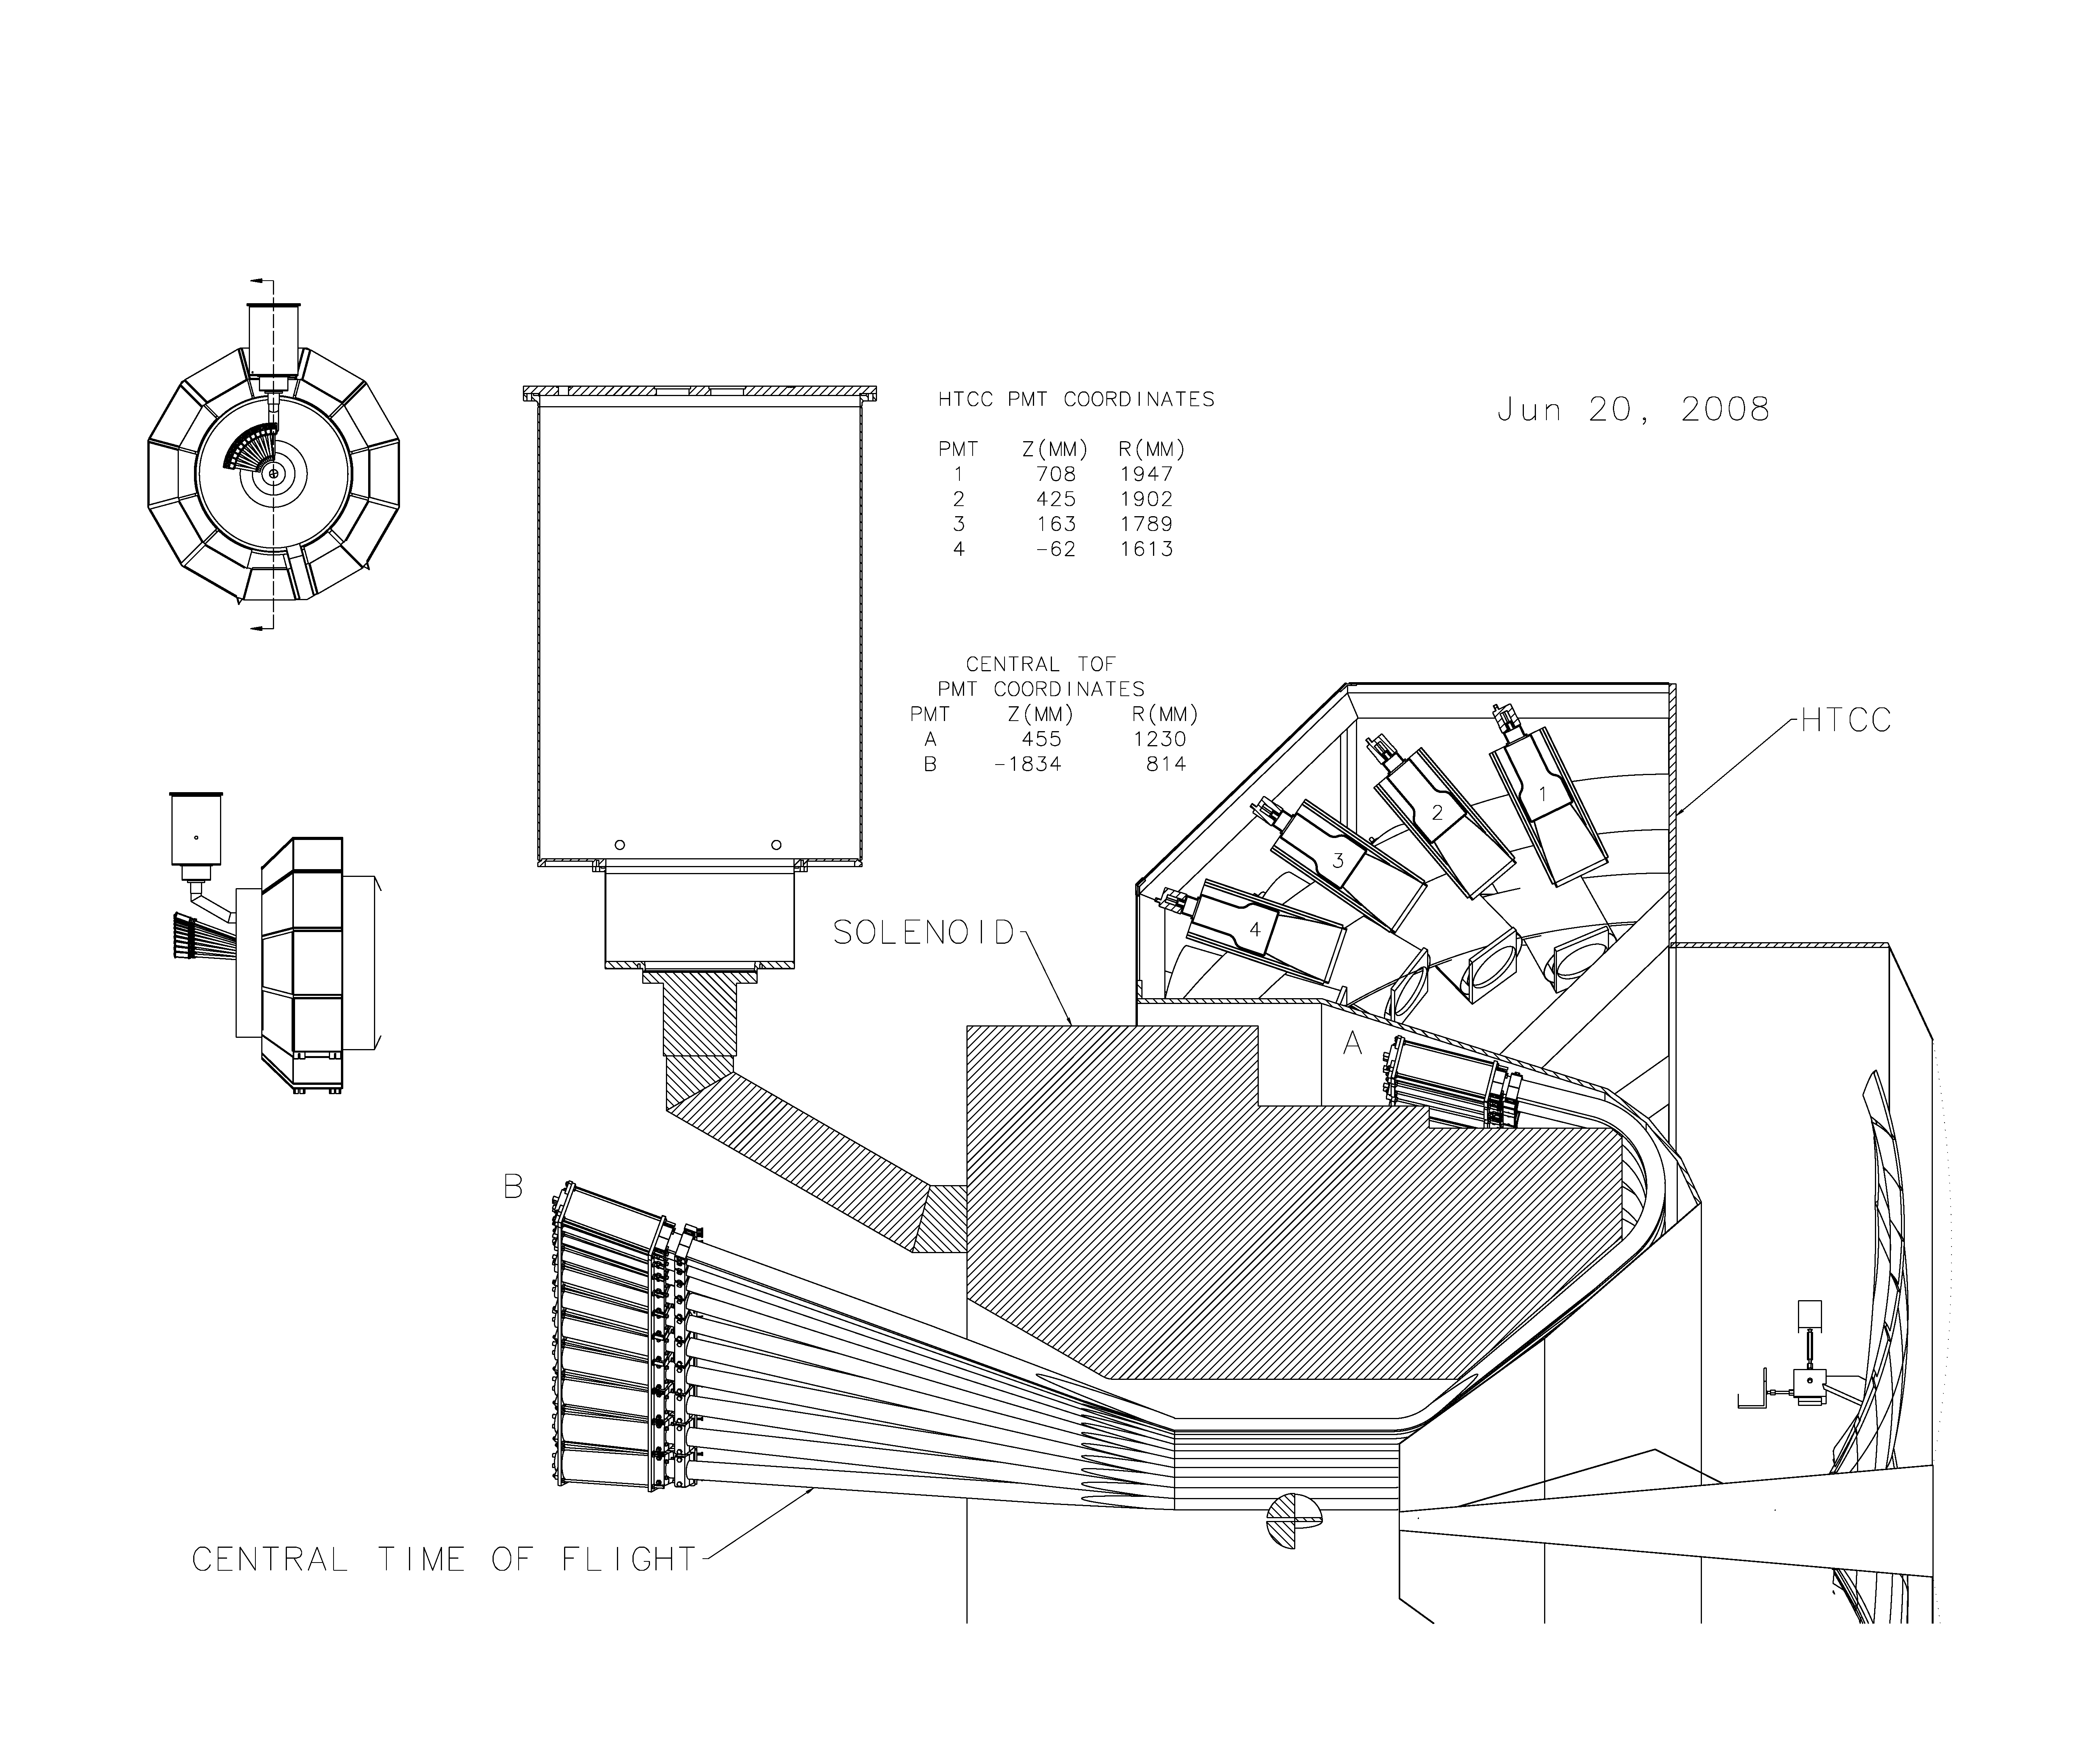
\includegraphics[width=17cm,clip=true,bb=100 600 2800 2000]{HTCC_CTOF_STUDY_060507_WRAP.ps.gz}
\end{center}
\caption{%CLASTOF.ps.gz.
Preliminary layout of the   CLAS Central TOF detector. 
Solenoid is shown as a hatched area. Scintillators form a barrel  66 cm long 
with the inner radius $24.945cm$.
Upstream and downstream,   light guides 
$50mm$ in diameter have a pitch of $7^o$ and $41^o$ respectively. 
The $1.5-1.7m$ long light guides for conventional PMTs
 may be replaced with $\approx1m$ long  light guides to accommodate 
magnetic field immune photo detectors. With this purpose a room 
 is  organized  at the outer downstream side of the solenoid casing.
The room for the magnetic shielding of the conventional PMTs 
may  be increased.
\label{barrel2}}
\end{figure}
\clearpage

%\begin{figure}[htbp]%#12
%\begin{center}
%%\includegraphics[width=13.4cm,clip=true,bb=-100 -40 730 850]{./figures_llg/mmap1.ps.gz}
%\includegraphics[width=17cm,clip=true,bb=100 600 8800 8000]{mmap1.ps.gz}
%\end{center}
%\caption{Layout of conventional PMTs at the magnetic field map.
% Downstream light guide and corresponding PMT are  shown in wite. For both PMTs the field is of $20T$.
%For magnetic immune photodetectors light guides may be  $/approx 0.8m$ long. The corresponding field 
%is of $ 0.6T$. 
%\label{barrel}}
%\end{figure}
%\clearpage
%%%%%%%%%%%%%%%%%%FIG.2%%%%%%%%%%%%%%%%%%%%%%
\begin{figure}[ht]
\vspace*{0.8cm}
\epsfverbosetrue\epsfxsize=15cm\epsfysize=15cm\epsfbox{mmap1.eps}
\vspace*{0.8cm}
\caption{Location of R2083 photo multipliers and magnetic field map.
         \label{fig:mmap1}}
\end{figure}
%%%%%%%%%%%%%%%%%%%%%%%%%%%%%%%%%%%%%%%%%%%%%
\clearpage


\begin{figure}[htbp]%#2
\begin{center}
%\includegraphics[width=13.8cm,clip=true,bb=-0 -40 720  800]{/home/prof/batourine/knu/publications/rep_llg_fromJLAB/cosmic-6pmtllg_picture.ps.gz}
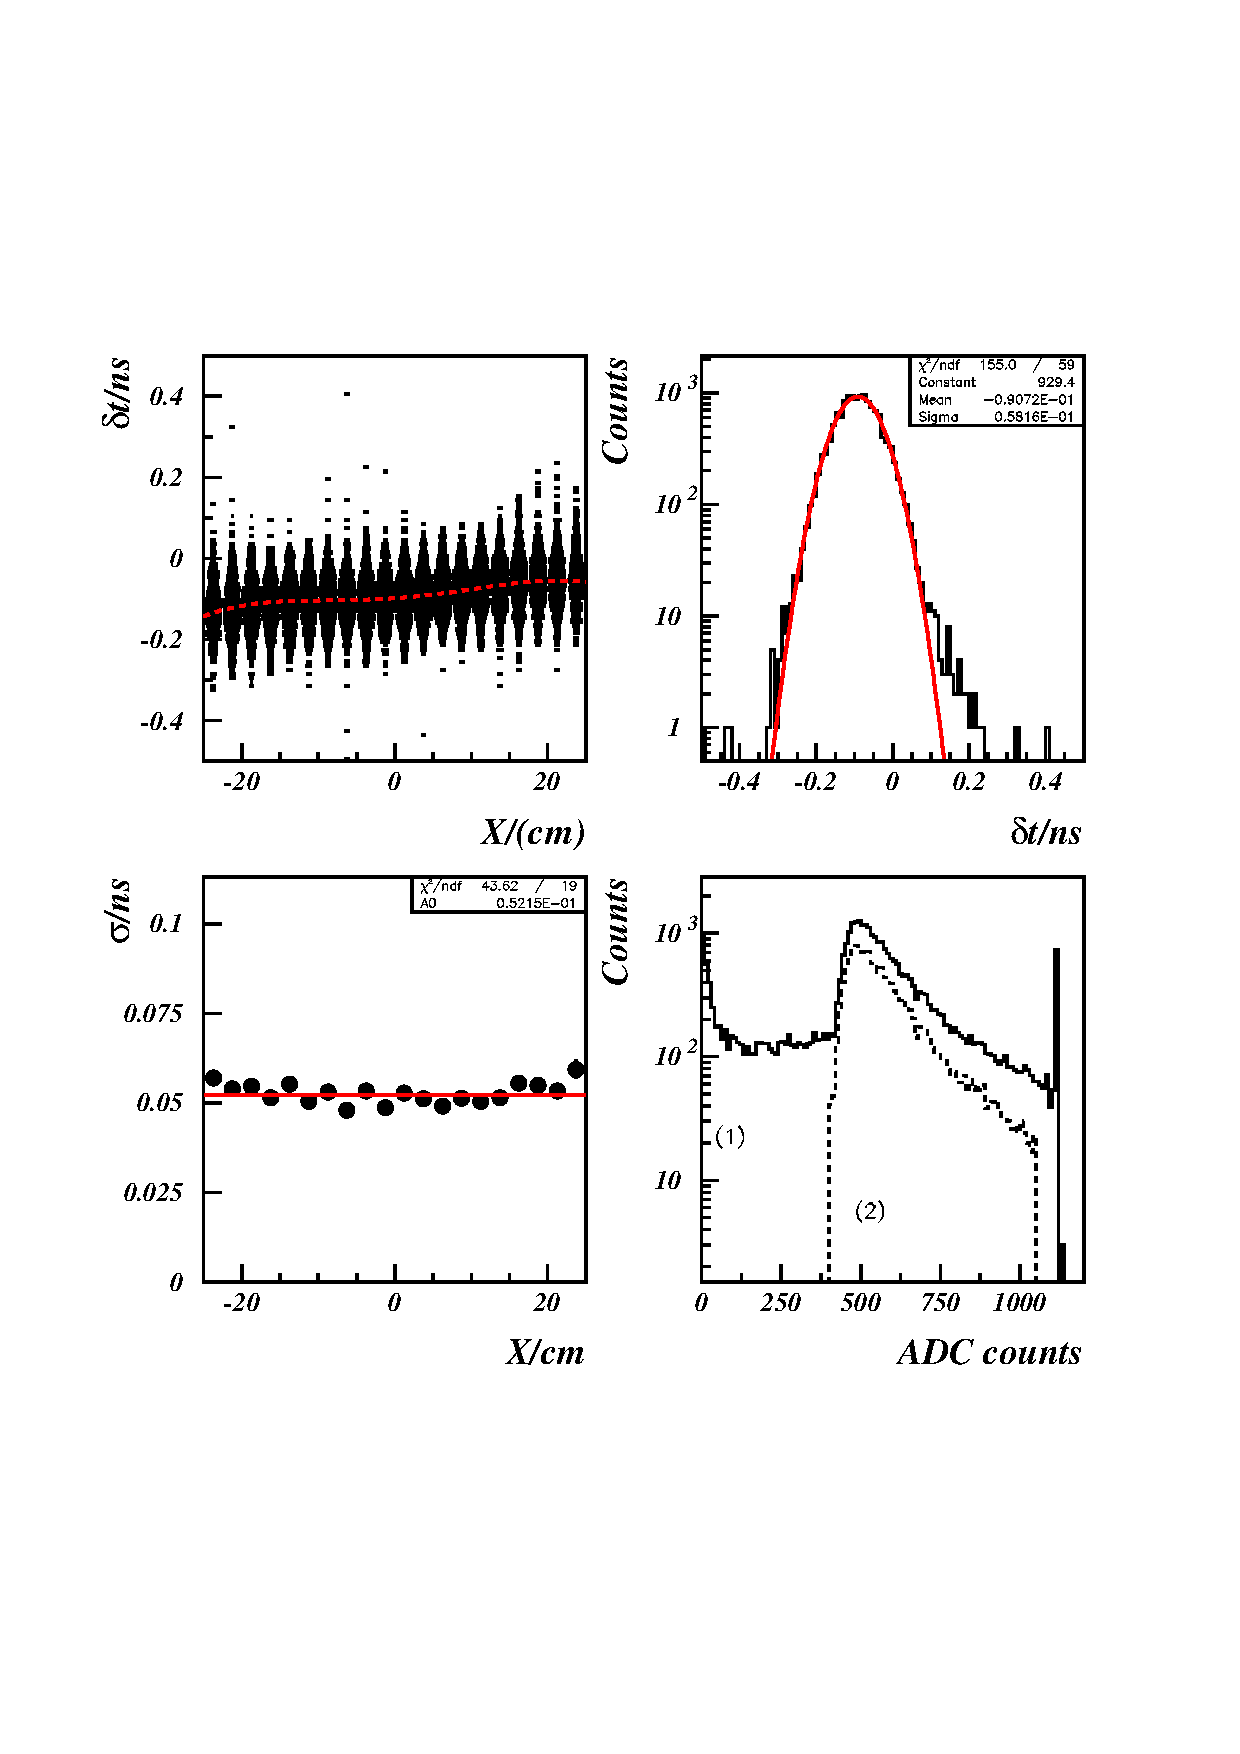
\includegraphics[width=13.8cm,clip=true,bb=20 150 620  720]{cosmic-6pmtnlg_picture.ps.gz}
\end{center}
\caption{%cosmic-6pmtnlg-picture.ps.gz,
Effective time resolution of R2083 PMT($\sigma$)
 in the reference triplet without 
light guides. Panel
1)top-left: scatter plot of residuals vs longitudinal coordinate $x$,
2)top-right: overall distribution of residuals with $\sigma_{R2083}=52.2\pm0.4~ps$, 
3)bottom-left: local $\sigma$ vs $x$,
4)bottom-right:  ADC values. Histogram (1) -raw events, histogram (2) - selected events when $both$ ADC values
are in the  span of this histogram.
\label{nlgres}}
\end{figure}


\begin{figure}[htbp]%#3
\begin{center}
\includegraphics[width=13.8cm,clip=true,bb=20 150 620  720]{cosmic-6pmtllg_picture.ps.gz}
\end{center}
\caption{%cosmic-6pmtllg-picture.ps.gz,
Effective time resolution of R2083 PMT in the reference triplet with $1m$ long strait 
light guides. Panel  
1)top-left:     scatter plot of residuals vs longitudinal coordinate $x$;
2)top-right:    overall distribution of residuals, $\sigma=77.9\pm0.6~ps$; 
3)bottom-left:  local $\sigma$ vs $x$ ;
4)bottom-right: ADC values. Histogram (1) -raw events, histogram (2) - selected events.
\label{lgres}}
\end{figure}
\clearpage


\begin{figure}[htbp]%#31
\begin{center}
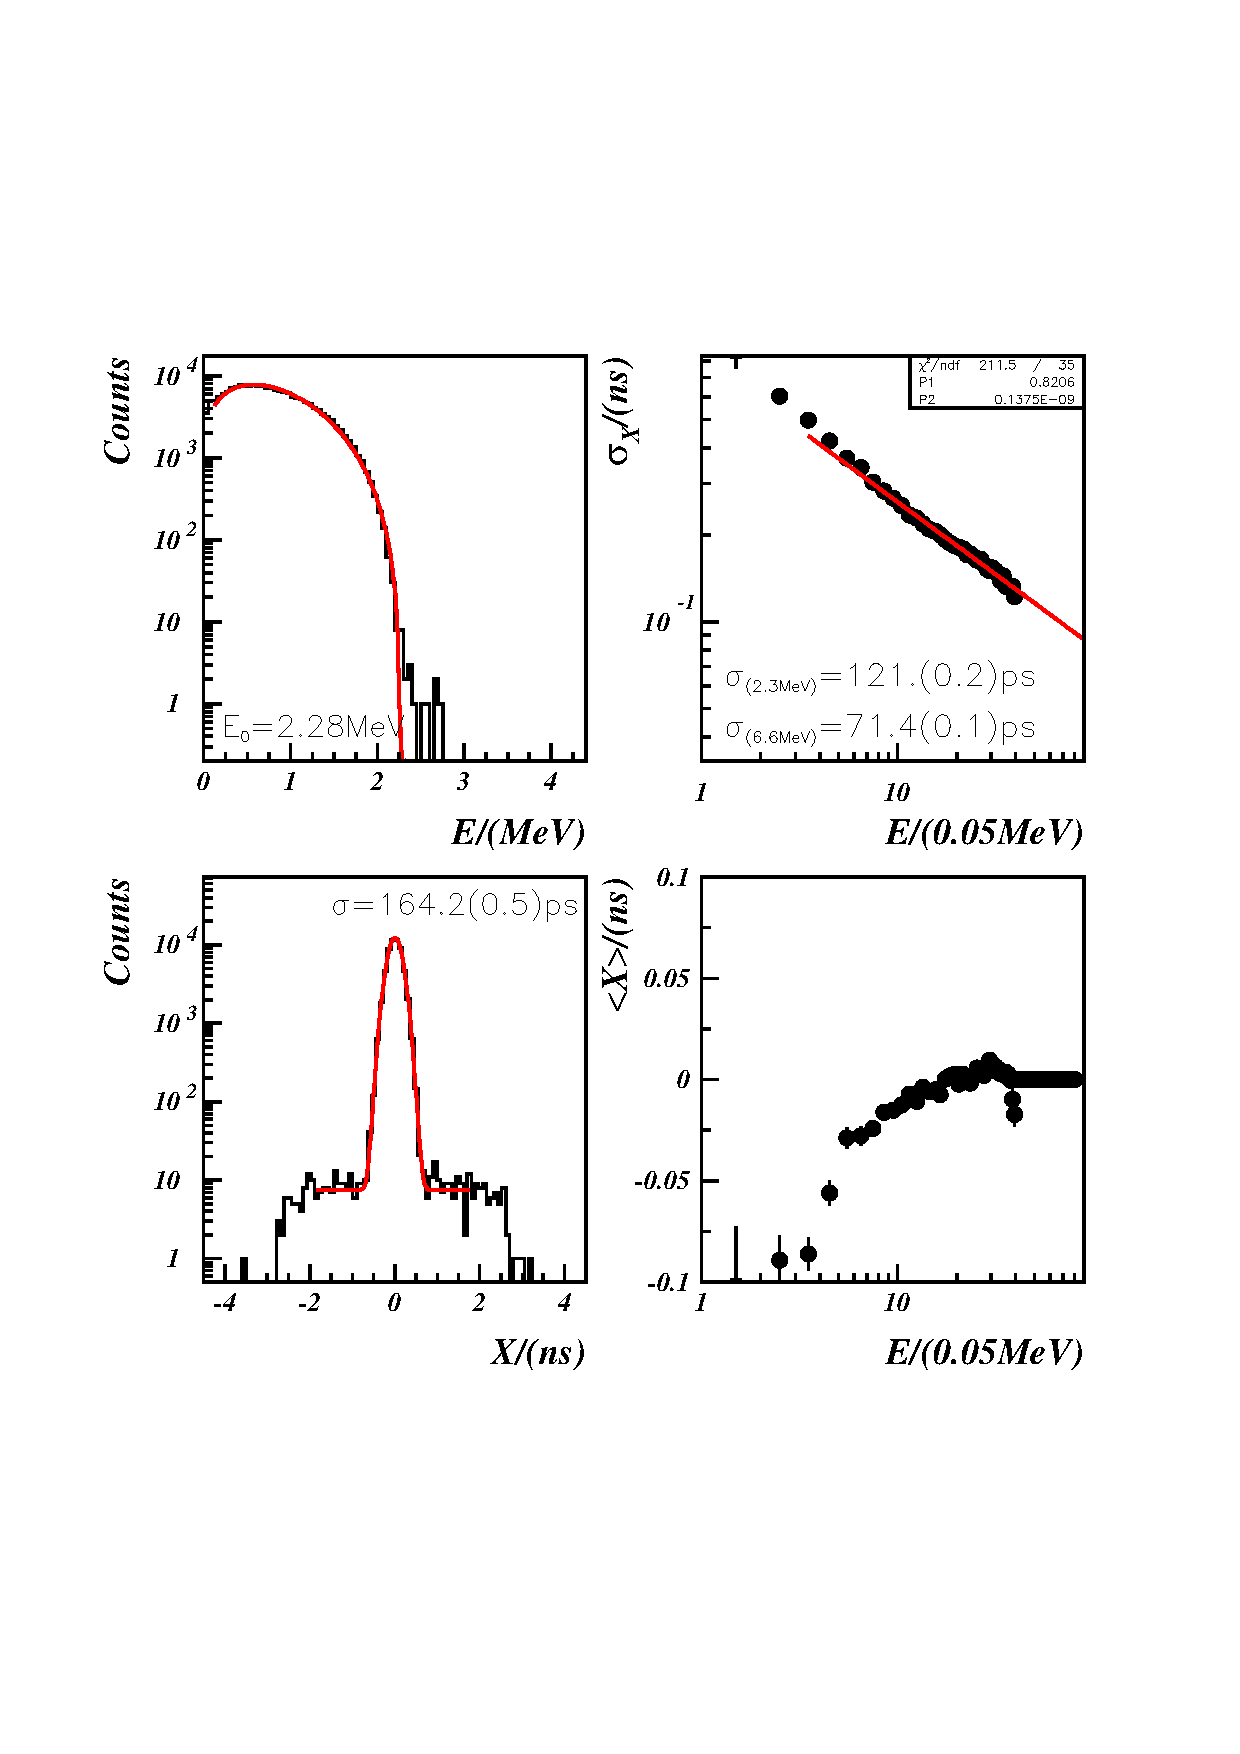
\includegraphics[width=13.8cm,clip=true,bb=20 150 620  720]{esxm_picture13.ps.gz}
\end{center}
\caption{
Effective time resolution of MCP PM Burle-85011   
obtained with the location method  of the 
 radiative source $^{90}Sr$   placed  in the center of the   counter.
Panel 
1)top-left: energy ($E$) spectrum of $\beta$-particles ;
2)bottom-left: coordinate distribution ($X$) of $\beta$-particles  with $E>1~MeV$; 
3)top-right: $\sigma_{X}$ of the peak vs $E$; 
4)bottom-right: $<X>$ vs  $E$.
\label{mcp85011sample}}
\end{figure}
\clearpage


\begin{figure}[htbp]%#32
\begin{center}
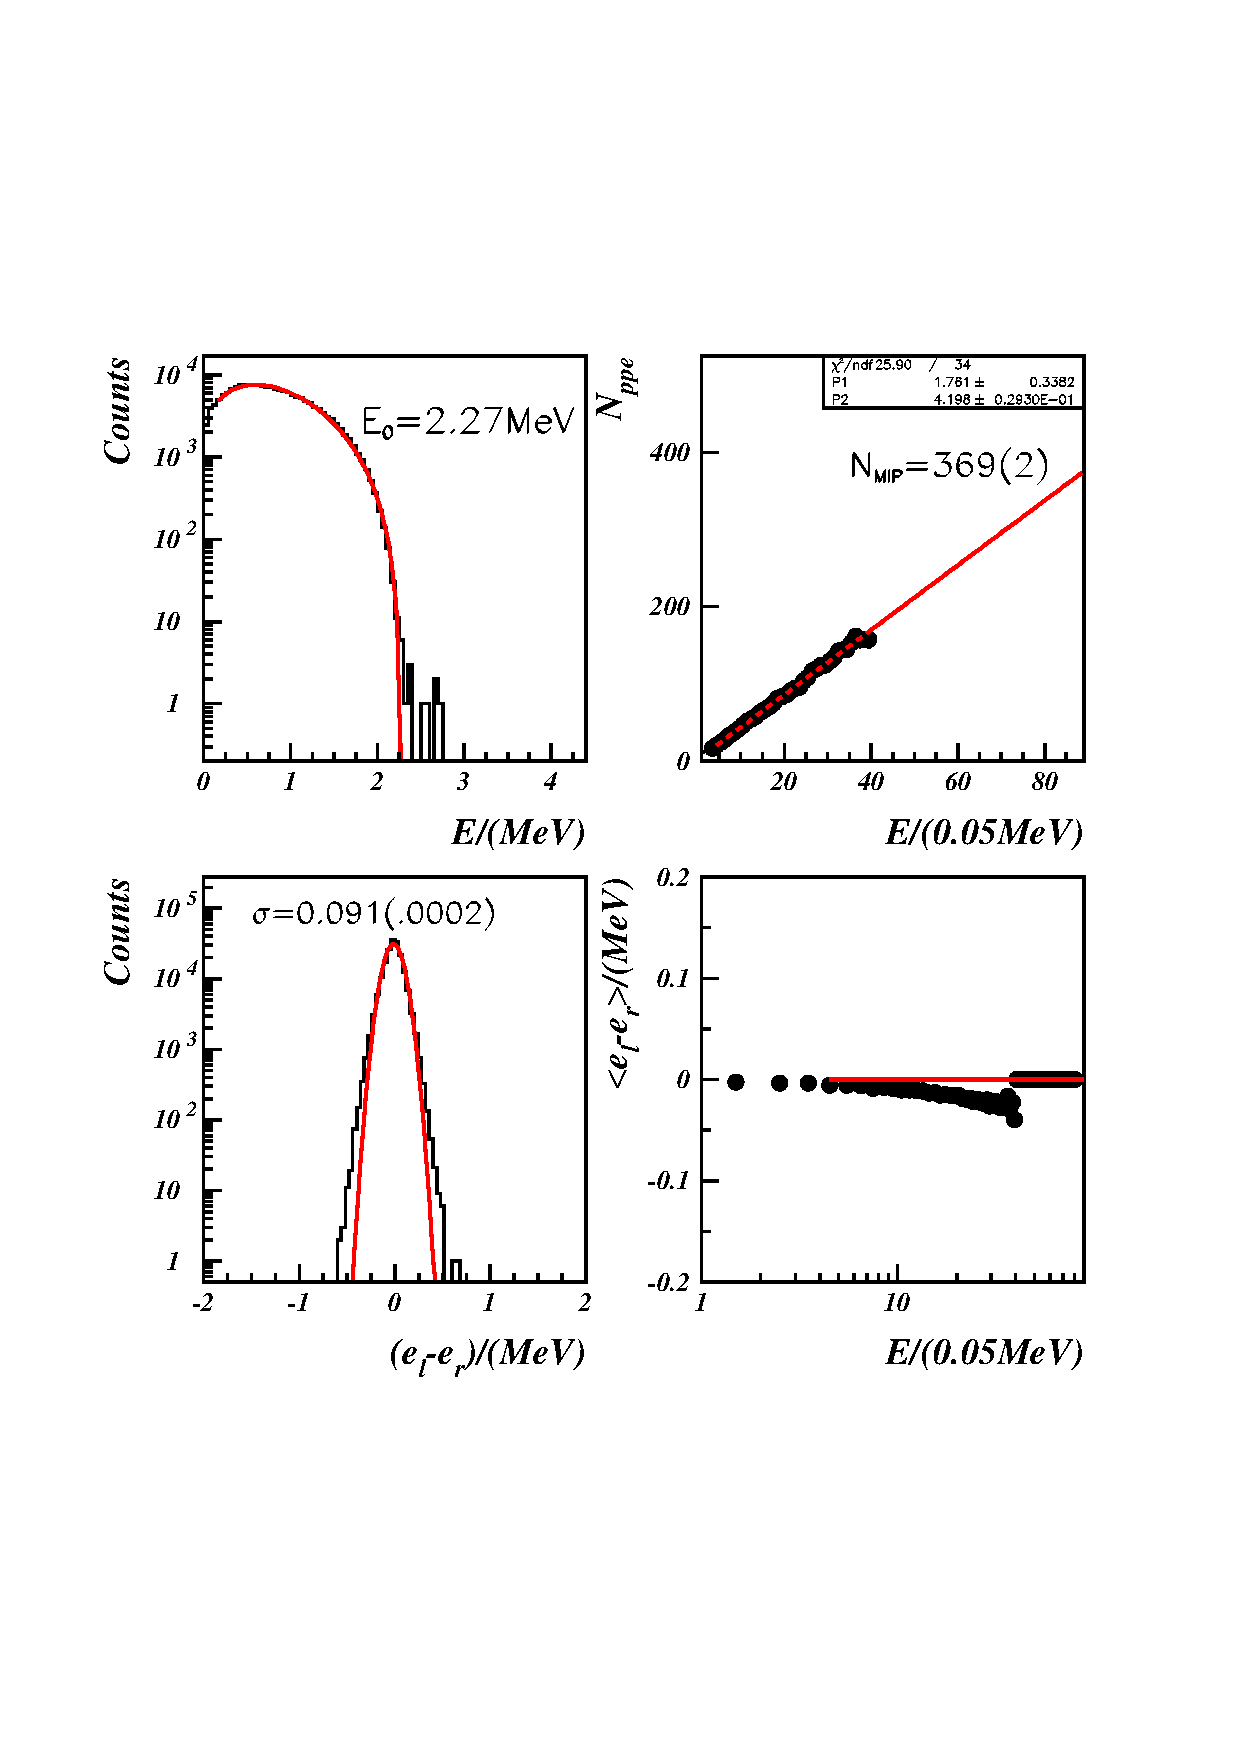
\includegraphics[width=13.8cm,clip=true,bb=20 150 620  720]{enppe_picture13.ps.gz}
\end{center}
\caption{Number of primary photoelectrons in Burle~85011.
1)Top-left: energy ($E$) spectrum of $\beta$-particles;
2)top-right:  $N_{ppe}$ vs $E$. It is expected to be $369\pm2$ at MIPs energy  $\approx4.4~MeV$;
3)bottom-left: spectrum of $(e_l-e_r)$, where $e_{l,r}$ are the energies measured from two sides of the counter;
4)bottom-right: mean value of $(e_l-e_r)$ vs  $\beta$-particle energy
\label{mcpnppe85011}}
\end{figure}
\clearpage


\begin{figure}[htbp]%#33
\begin{center}
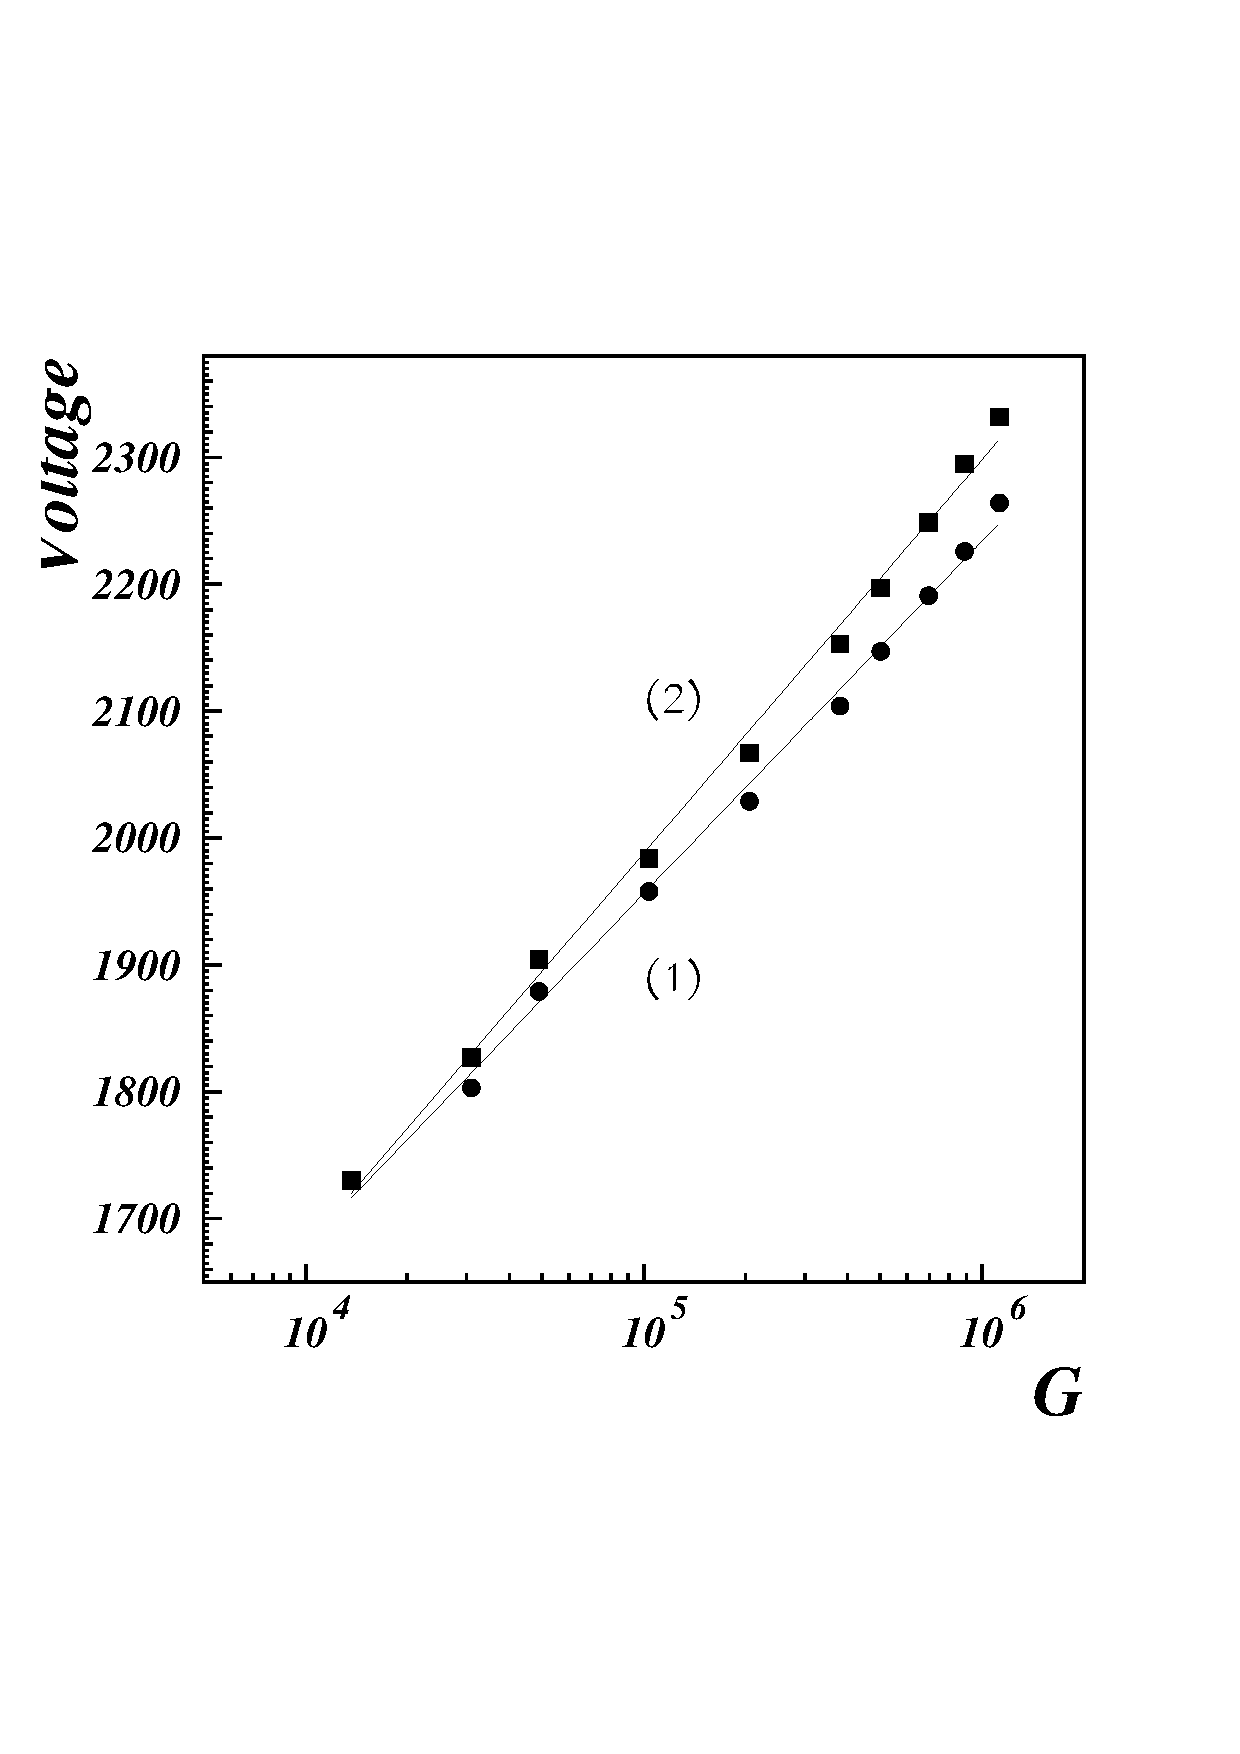
\includegraphics[height=13.8cm,clip=true,bb=20 150 620  720]{hvvsgain_picture85011.ps.gz}
\end{center}
\caption{High Voltage  vs Burle~85011 Gain.
The curves (1) and (2) are fits to the power law.
(1)-left  PM,(2)-right  PM.}
\label{hvvsgain85011}
\end{figure}
\clearpage

\begin{figure}[htbp]%#34
\begin{center}
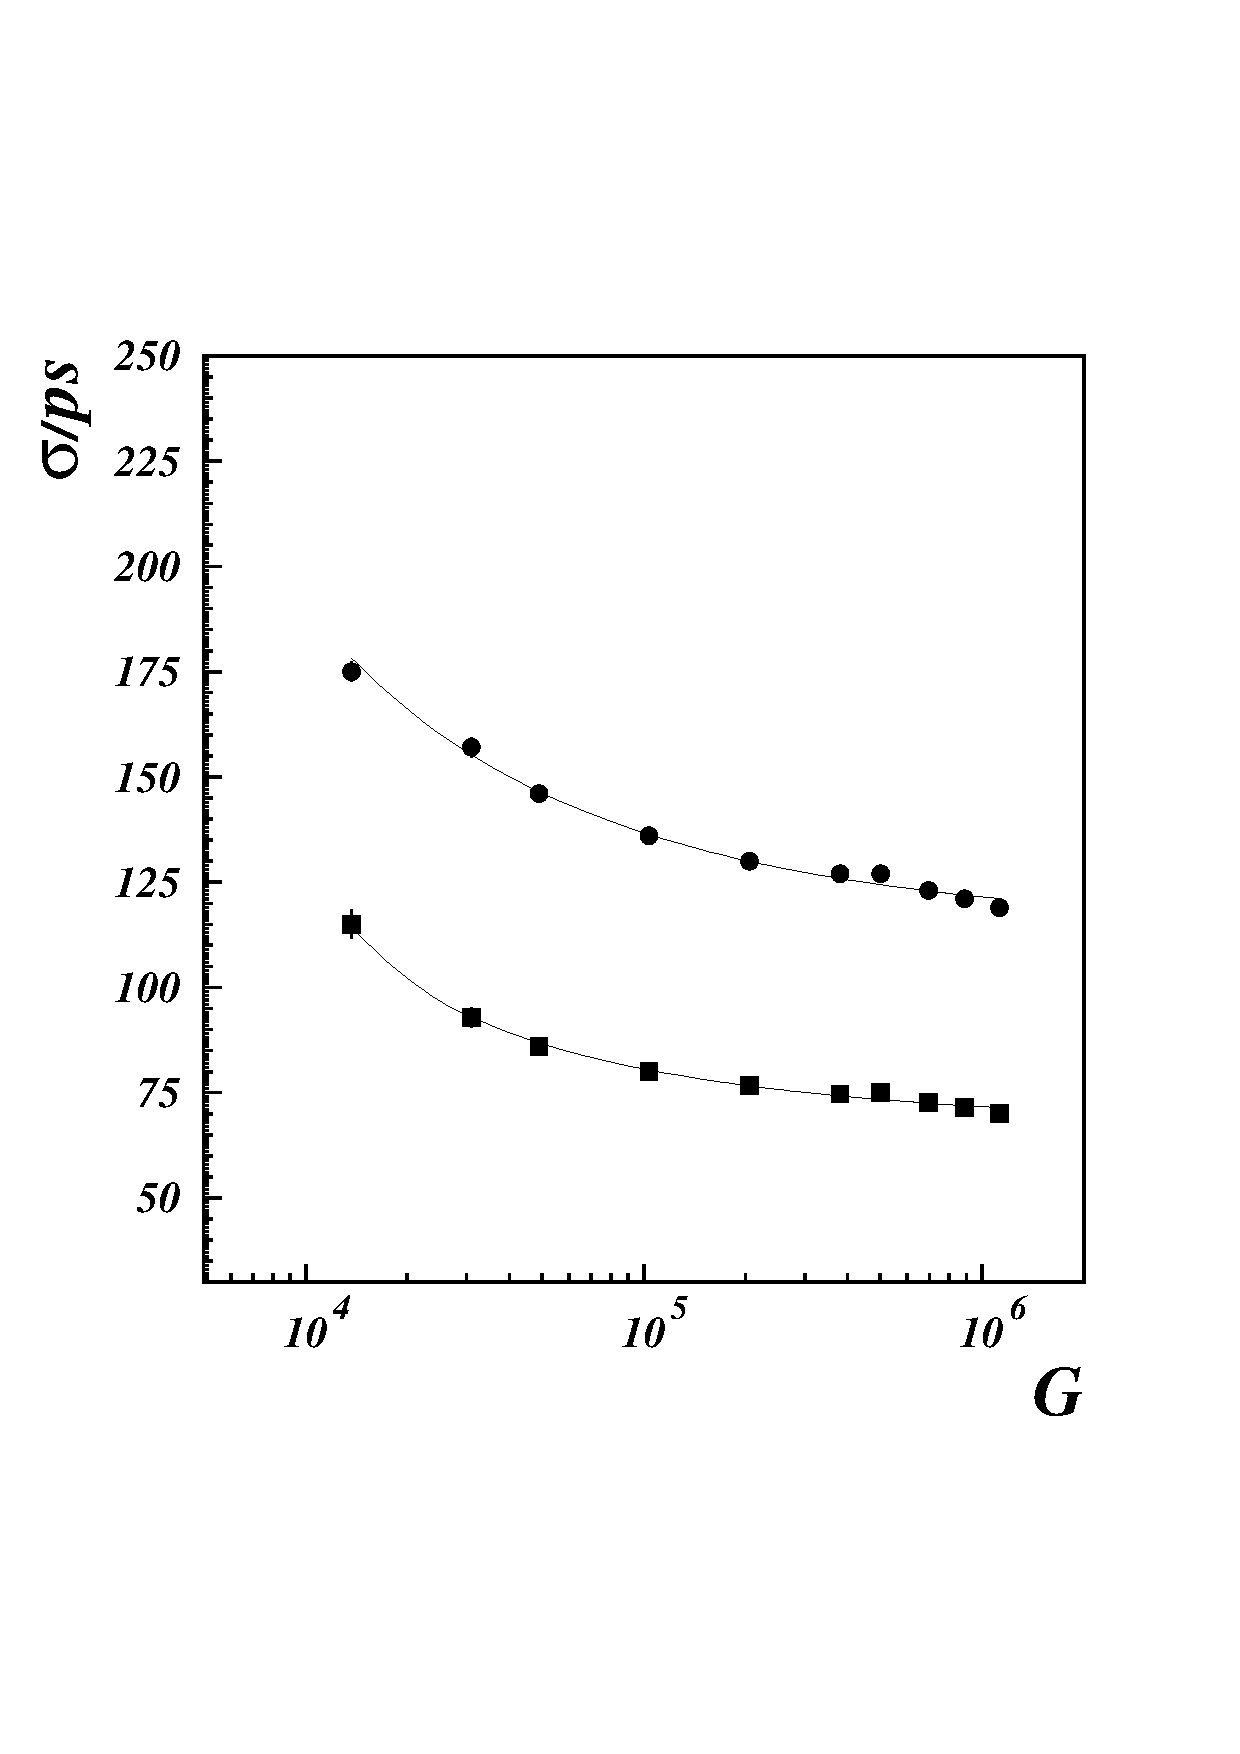
\includegraphics[height=13.8cm,clip=true,bb=20 150 620  720]{res85011vsgain_picture85011.ps.gz}
\end{center}
\caption{Resolution  of Burle~85011  vs gain(G). 
Circles are for the $\sigma$ at ${\Delta}E=2.28MeV$.
Squares are for extrapolation to  ${\Delta}E=6.6MeV$~(corresponds to MIPs in $3~cm$ thick scintillator).
The curves are  fits to the $G^{-2}$ dependence.  
Amplification factor to the PM signals is 50.}
\label{sigmamip85011}
\end{figure}

\clearpage

%\caption{Spectra of residual  measured with 
%%         two R7761-70 and four R2083 PMTS(right) and six R2083 PMTs.
%%         \label{fig:res}}
%\end{figure}
%%%%%%%%%%%%%%%%%%%%%%%%%%%%%%%%%%%%%%%%%%%%
%%\begin{figure}[htbp]%#35
%%\begin{center}
%%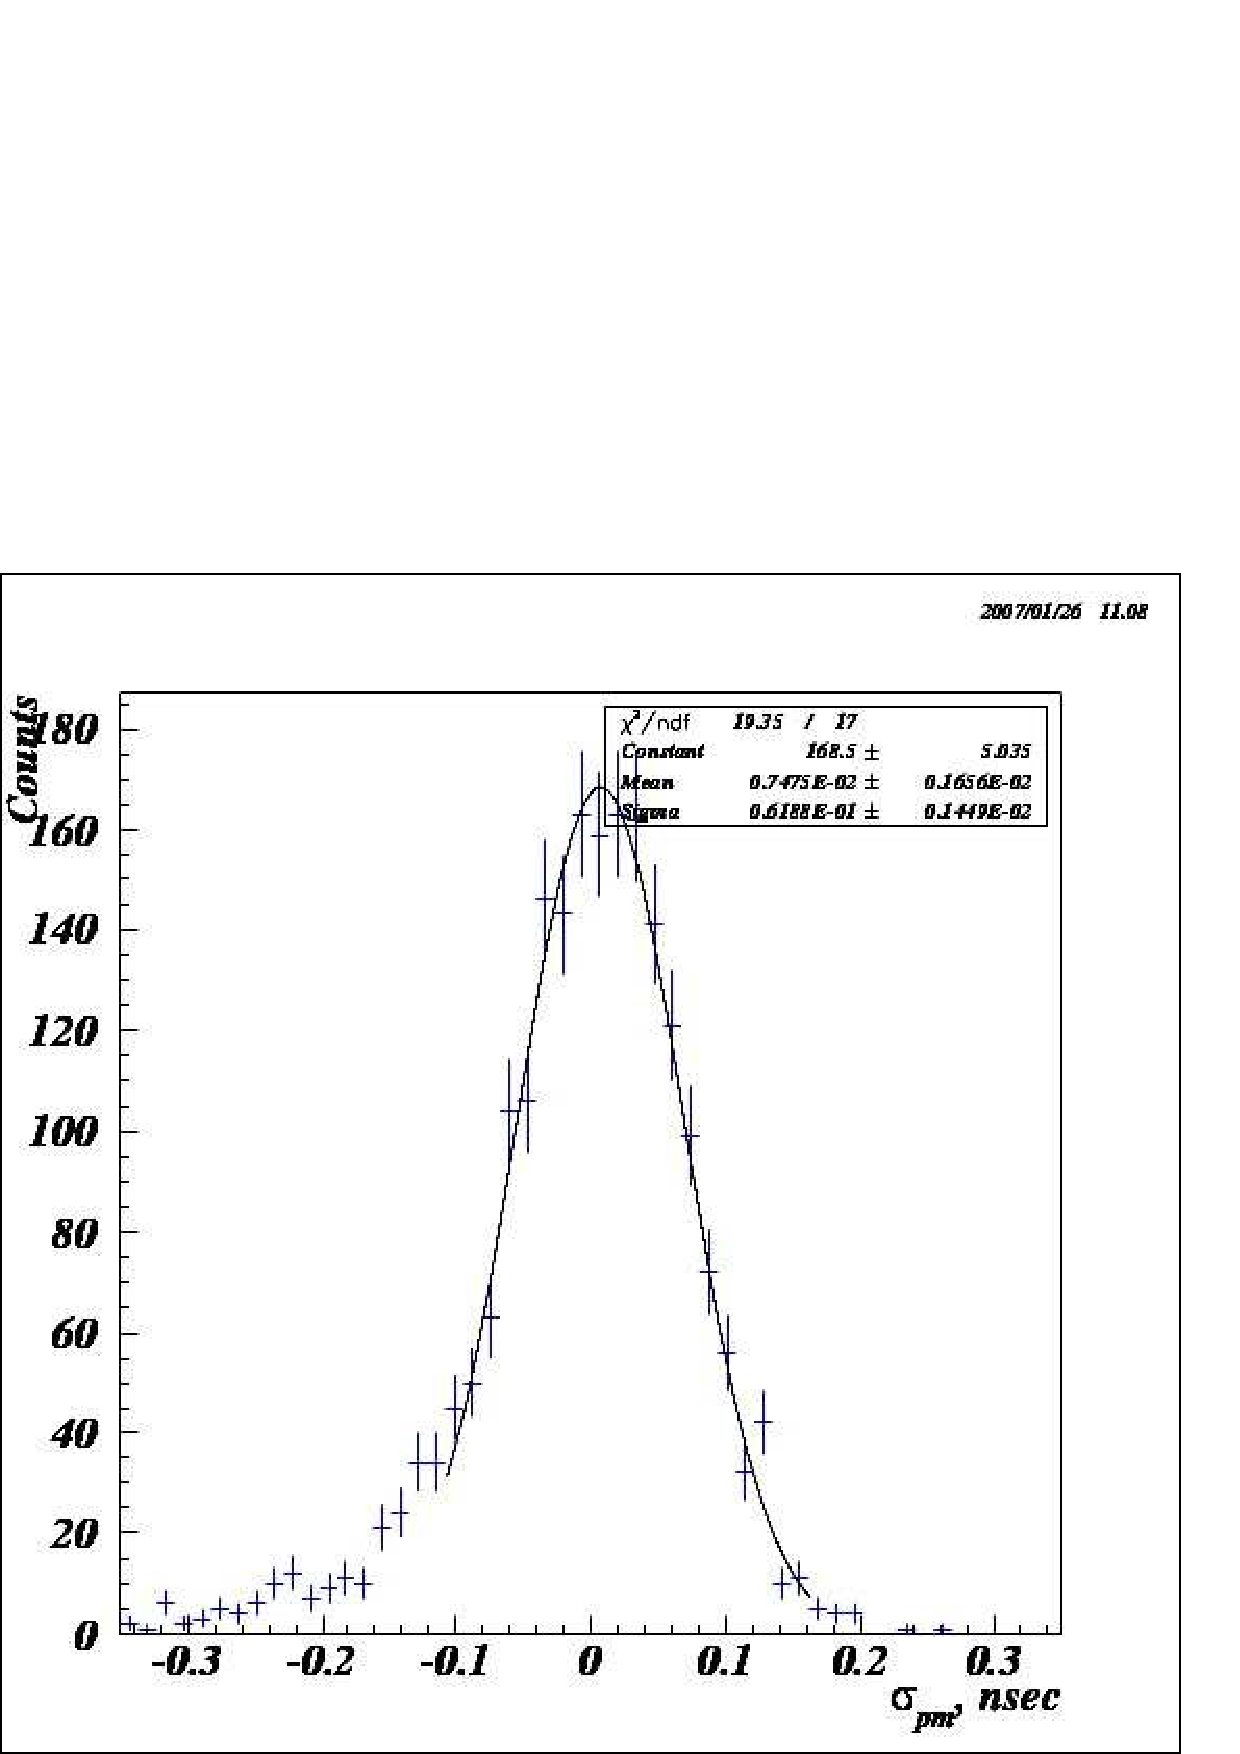
\includegraphics[height=13.8cm,clip=true,bb=20 0 620  720]{res5505.ps.gz}
%%\end{center}

%%%%%%%%%%%%%%%%%FIG.2%%%%%%%%%%%%%%%%%%%%%%
\begin{figure}[ht]
\vspace*{0.2cm}
\epsfverbosetrue\epsfxsize=6.5cm\epsfysize=7cm\epsfbox{tau041007.eps}
\hspace*{0.4cm}\epsfverbosetrue\epsfxsize=6.5cm\epsfysize=7cm\epsfbox{tau0117a.eps}
\vspace*{-0.3cm}
\caption{Spectra of 6 PMT time residuals scaled by $\frac{2}{\sqrt{3}}$.
 Left panel: distribution  with two R7761-70 and four R2083 PMTS(right).  
Right panel: distribution obtained with with  six R2083 PMTs.
The actual effective  $\sigma_{R7761}=64~ps$ yields from the $rms$ of the  left  panel.
The  reference  $\sigma_{R2083}=52\pm1ps$ at the right  panel  
coincides with the previously reported value from Table~\ref{crt}.
\label{finemesh01}}
\end{figure}
\clearpage

\begin{figure}[htbp]%#4
\begin{center}
%\includegraphics[width=13.8cm,clip=true,bb=-0 -40 720  800]{/home/prof/batourine/knu/publications/rep_llg_fromJLAB/cosmic-6pmtllg_picture.ps.gz}
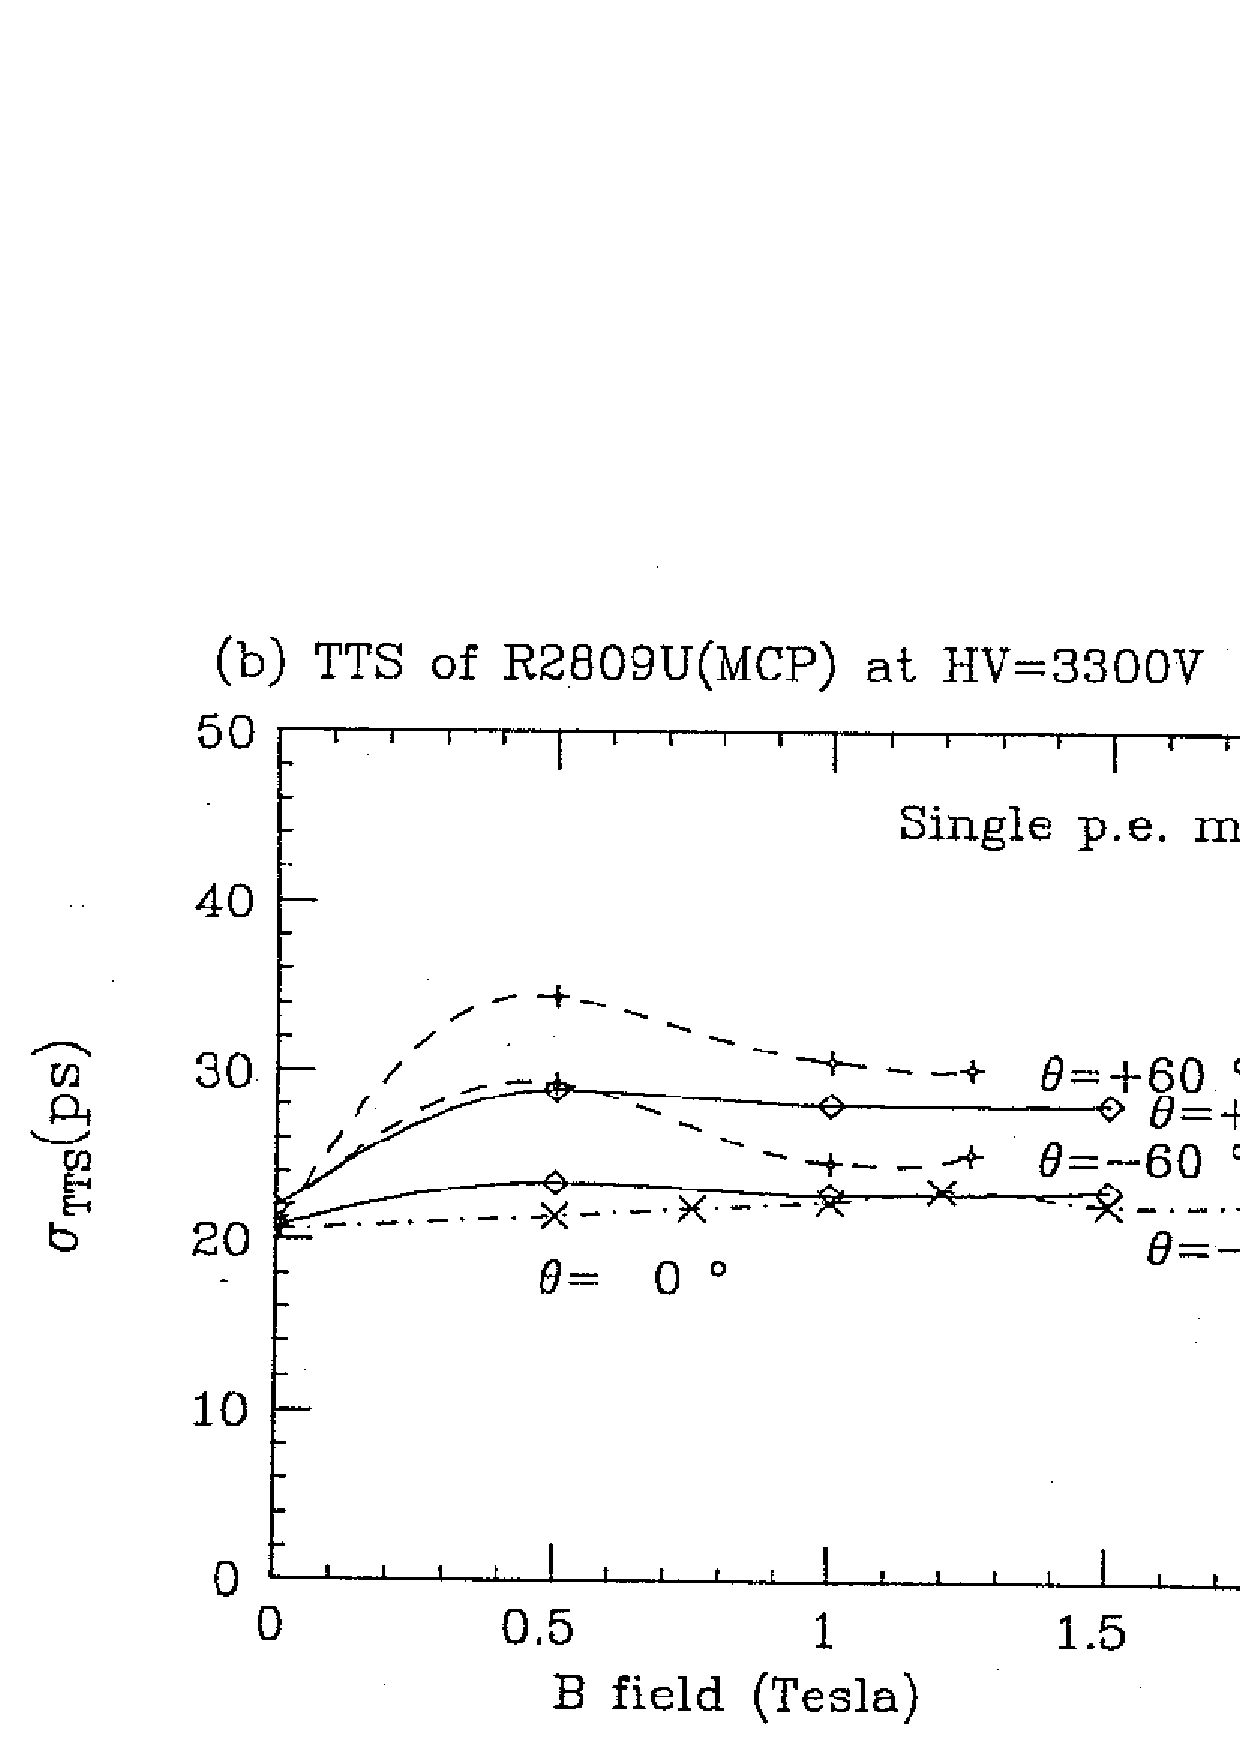
\includegraphics[width=13.8cm,clip=true,bb=20 150 620  720]{fig02MC.ps.gz}
\end{center}
\caption{%fig02MC.ps.gz,
Transition Time Spread of the MCP PM  vs magnetic field.
\label{mcpt}}
\end{figure}
\clearpage

\begin{figure}[htbp]%#5
\begin{center}
%\includegraphics[width=13.8cm,clip=true,bb=-0 -40 720  800]{/home/prof/batourine/knu/publications/rep_llg_fromJLAB/cosmic-6pmtllg_picture.ps.gz}
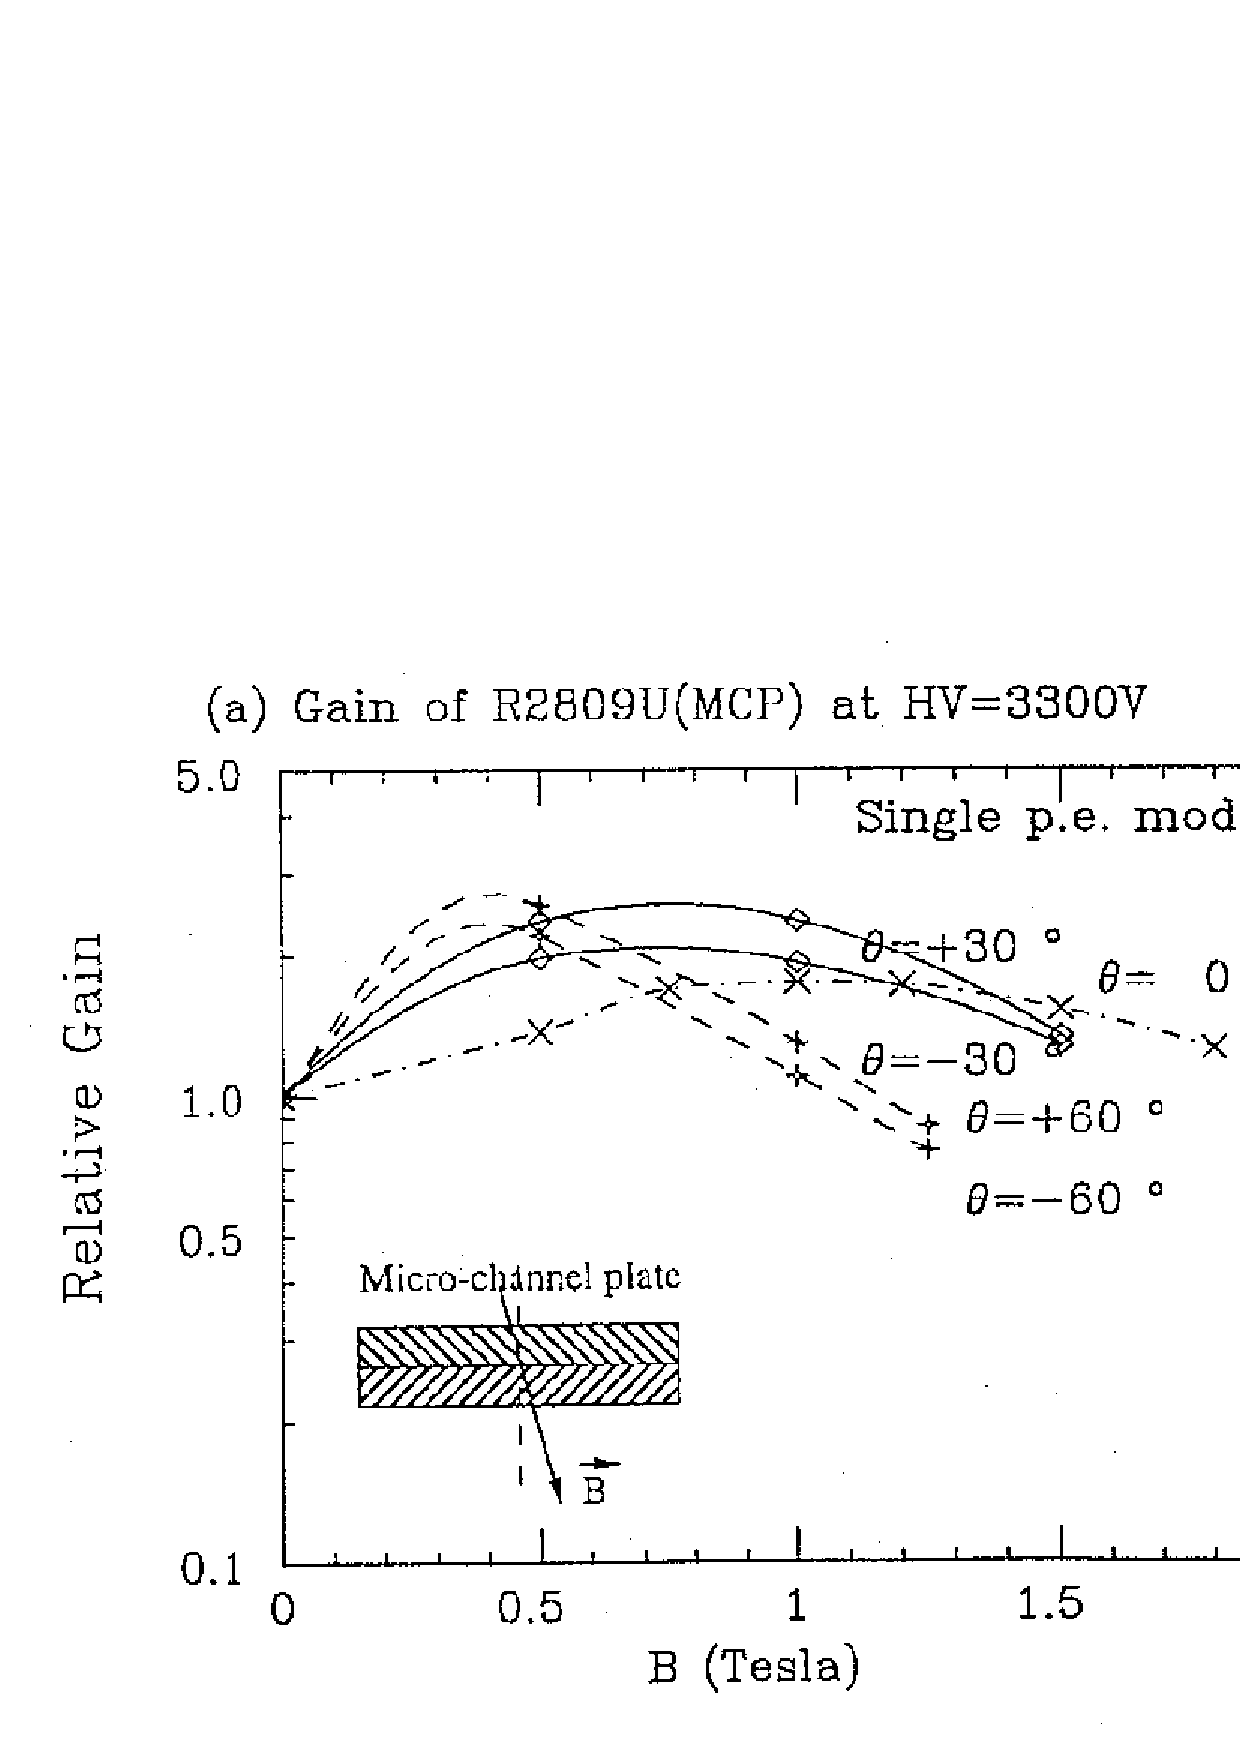
\includegraphics[width=13.8cm,clip=true,bb=20 150 620  720]{fig01MC.ps.gz}
\end{center}
\caption{%fig01MC.ps.gz,
Gain of the MCP PM  vs magnetic field at different orientations. 
\label{mcpg}}
\end{figure}
\clearpage



\begin{figure}[htbp]%#6
\begin{center}
%\includegraphics[width=13.8cm,clip=true,bb=-0 -40 720  800]{/home/prof/batourine/knu/publications/rep_llg_fromJLAB/cosmic-6pmtllg_picture.ps.gz}
\includegraphics[width=13.8cm,clip=true,bb=20 150 620  720]{fig03MC.ps.gz}
\end{center}
\caption{%fig03MC.ps.gz,
Gain of the fine mesh PM R2490-05 vs magnetic field at different orientations. 
\label{fmg}}
\end{figure}
\clearpage


\begin{figure}[htbp]%#7
\begin{center}
%\includegraphics[width=13.8cm,clip=true,bb=-0 -40 720  800]{/home/prof/batourine/knu/publications/rep_llg_fromJLAB/cosmic-6pmtllg_picture.ps.gz}
\includegraphics[width=13.8cm,clip=true,bb=20 150 620  720]{fig04MC.ps.gz}
\end{center}
\caption{%fig04MC.ps.gz,
Transition Time Spread of the fine mesh PM R2490-05 vs magnetic field.
\label{fmt}}
\end{figure}
\clearpage


\begin{figure}[htbp]%#8
\begin{center}
%\includegraphics[width=14cm,clip=true,bb=80 0 550  800]{/home/prof/batourine/fig/bentlg03.ps.gz}
%\includegraphics[width=14cm,clip=true,bb=55 0 550  750]{./bentlg03.ps.gz}
\includegraphics[width=22cm,clip=true,bb=100 40 750 590]{JLABt0R2083-2.ps.gz}
\end{center}
\caption{%JLABt0R2083-2.ps.gz
The pilot design  of the CLAS12 CTOF counter.
 (1)-PMT R2083 from Hamamatsu, (2)- acrylic light guides,
(4)-supporting cones and rings, (3)-scintillators.
Magnetic field is shown by vectors.
\label{bentlg03}}
\end{figure}
%\addtocontents{lof}{List of figures}
\clearpage


\newpage
\begin{figure}[htbp]%[h]#9
\begin{center}
%\includegraphics[height=17cm,clip=true,bb=100 0 500  760]{/home/prof/batourine/fig/bentlgupdownstream.ps.gz}
\includegraphics[height=17cm,clip=true,bb=100 0 500  760]{bentlgupdownstream.ps.gz}
\end{center}
\caption{%bentlgupdownstream.ps.gz,
Upstream (1) and downstream (2) view of the CTOF detector.
\label{bentlgud03}}
\end{figure}
\clearpage

%
\newpage
\begin{figure}[htbp]%#10
\begin{center}
%\includegraphics[height=14cm,clip=true,bb=75 100 555  680]{/home/prof/batourine/fig/t0sccross.ps.gz}
\includegraphics[height=14cm,clip=true,bb=75 100 555  680]{t0sccross.ps.gz}
\end{center}
\caption{%t0sccross.ps.gz,
The cross section of the scintillator inscribed into the 
photo-cathode of R2083 from Hamamatsu.  
Light guides will  join PMTs via the
cylindrical side of the same diameter as
the  R2083 photo-cathode, i.e. $46~mm$. 
\label{sccross}}
\end{figure}
\clearpage


\newpage

\begin{figure}[htbp]%#11
\begin{center}
%\includegraphics[width=13.8cm,clip=true,bb=-0 -40 720  800]{/home/prof/batourine/knu/publications/rep_llg_fromJLAB/transitionvscyl.ps.gz}
\includegraphics[width=13.8cm,clip=true,bb=20 100 620  720]{transitionvscyl.ps.gz}
\end{center}
\caption{%transitionvscyl.ps.gz,
The light transportation efficiency(vertical scale)  of the ``pyramid'' light guide vs the length 
(horizontal scale) of the milled surface.
\label{plgef}}
\end{figure}
\clearpage


\begin{figure}[htbp]%#12
\begin{center}
%\includegraphics[width=13.8cm,clip=true,bb=-0 80 700 800]{/home/prof/batourine/fig/t0lgupstr.ps.gz}
\includegraphics[width=13.8cm,clip=true,bb=-0 -40 600 800]{t0lgupstr.ps.gz}
\end{center}
\caption{%t0lgupstr.ps.gz,
The design of the upstream light guide.
\label{lgupstream}}
\end{figure}
\clearpage

%\newpage
%\begin{figure}[h]%#13
%\begin{center}
%\includegraphics[width=13.8cm,clip=true,bb=-0 -40 320  300]{./figures_llg/polishingLightGuide3.eps}
%\end{center}
%\caption{Manufacturing the $1m$-long light guides.}
%\label{lgmanu}
%\end{figure}

\clearpage
\newpage
\begin{figure}[htbp]%#13
\begin{center}
%\includegraphics[width=13.8cm,clip=true,bb=-0 -80 700 800]{/home/prof/batourine/fig/t0lgdown.ps.gz}
\includegraphics[width=13.8cm,clip=true,bb=-0 -40 600 800]{t0lgdown.ps.gz}
\end{center}
\caption{%t0lgdown.ps.gz,
The design of the downstream   $1m$-long light guide}
\label{lgdownstream}
\end{figure}
\clearpage


\begin{figure}[htbp]%#14
\begin{center}
%\includegraphics[width=13.8cm,clip=true,bb=-0 -40 720  800]{/home/prof/batourine/knu/publications/rep_llg_fromJLAB/transitionvscyl.ps.gz}
\includegraphics[width=13.8cm,clip=true,bb=20 100 620  720]{trans.ps.gz}
\end{center}
\caption{%trans.ps.gz,
Light transmission  vs 1) the ``down mirror'' orientation angle(left panel)
2) the reflectivity of the light guide surface(right panel).
\label{trans}}
\end{figure}
\clearpage

\begin{figure}[htbp]%#15
\begin{center}
%\includegraphics[width=14cm,clip=true,bb=80 0 550  800]{/home/prof/batourine/fig/bentlg03.ps.gz}
\includegraphics[height=20cm,clip=true,bb=55 0 550  780]{JLABt0H8500.ps.gz}
\end{center}
\caption{%JLABt0H8500.ps.gz,
The design  of the CLAS12 CTOF counter with 
H8500 from Hamamatsu. Acrylic light guides are rectangular in 
cross section at the photo-cathode($49\times49~mm^2$). The length of
 the upstream/downstream light guides is $863/441~mm$, respectively.
At the scintillator end LG's, as well as  ``Bicron-408'', are 
 trapezoids in cross section. At the PMT side they are squared.
Magnetic fields are shown with vectors.
\label{JLABt0H8500}}
\end{figure}
\clearpage

\newpage 
\begin{figure}[htbp]%#16
\begin{center}
%\includegraphics[width=14cm,clip=true,bb=80 0 550  800]{/home/prof/batourine/fig/bentlg03.ps.gz}
\includegraphics[height=14cm,clip=true,bb=55 30 550  820]{JLABt0H85011.ps.gz}
\end{center}
\caption{%JLABt0H85011.ps.gz,
General view of the CLAS12 CTOF counter with MCP PMs 85011 from Burle.
(1)mirror film,(2) two adjacent scintillators,(3)-Burle85011 multi-anode assembly.
\label{JLABt0H85011}}
\end{figure}
\clearpage


\begin{figure}[htbp]%#17
\begin{center}
%\includegraphics[width=14cm,clip=true,bb=80 0 550  800]{/home/prof/batourine/fig/bentlg03.ps.gz}
\includegraphics[width=14cm,clip=true,bb=0 0 620  700]{JLABH85011.ps.gz}
\end{center}
\caption{%JLABH85011.ps.gz,
The closer view of  the CLAS12 CTOF counter with MCP PMs 85011 from Burle. 
\label{JLABH85011}}
\end{figure}
\clearpage


\begin{figure}[htbp]%#18
\begin{center}
%\includegraphics[width=14cm,clip=true,bb=80 0 550  800]{/home/prof/batourine/fig/bentlg03.ps.gz}
\includegraphics[width=14cm,clip=true,bb=55 30 550  820]{JLABH85011-1.ps.gz}
\end{center}
\caption{%JLABH85011-1.ps.gz,
Staggering CTOF counters with MCP PMs 85011 from Burle. 
\label{JLABH85011-1}}
\end{figure}
\clearpage

 

\end{document}



\subsection{Evaluation of the Design.}
%In order to simplify the   $R\&D$ for the production of bent  light guides
We have to address the following questions which may have a dramatic impact on the design.
%\begin{itemize}
%\item
\subsubsection{Opening angle.}
\paragraph{Is the opening angle enough in the suggested design?}
The downstream light guide has a `` focusing mirror'' on the inner surface of the barrel.
The length of this  mirror   is $17.3~mm$, that  reduces the opening angle of the downstream side.
We note that, since $\theta_{br}=sin^{-1}(1.49)\approx42^o$ for acrylic, the length of the mirror has to be 
at least $30.5~tg(\theta_{br})=28~mm$.
This mirror may be avoided in the design,
 but in such case some light will be reflected back 
into the scintillator.
This question may be solved by comparing  Monte-Carlo calculations\cite{mutch} for different dimensions.
\subsubsection{Cerenkov's light.}
\paragraph{Do we care about the Cerenkov light in the light guides?}
The relatively thick light guides may be a source of handicapping Cerenkov light, especially
if tracks are oriented along the $22^0$ or $45^0$ pitch of  light guides.
What is the limitation caused  by  the Cerenkov light? 
This question may be only addressed in the general MC simulation of the detector.
 However, one can consider using non-UVT acrylic, which transmits
most of the blue scintillator light but cuts off the Cerenkov UV thereby
suppressing background in the light guides.

\subsubsection{``Start'' counter and Solenoid.}
\paragraph{General shape of the ``start counter''detector.}
We have to estimate the suggested design from the point of view of other components of 
the central detector, in particular with respect to the Solenoid. 
Also, this  design requires  supporting rings for 100  light guides,
and PMTs in a heavy metal case   with total weight of $\approx1000~KG$ which may crate problems for 
other detector components.  






%Information about plastics may be found at
%http://www.3d-cam.com/materials/acrylic.asp


\subsection{Transport efficiency of light guides.}
We have calculated the transport efficiency of the light guides using the code BARTIM described in the Appendix of reference \cite{mutch}. 
In this Monte Carlo program a photon is either totally internally reflected or reflected or refracted according to the Fresnel equations. 
Imperfections on the surface are modeled by reducing the total internal reflection co-efficient, IR, below 100\%. 
The light that escapes the scintillator (or light guide) is specularly reflected with the appropriate reflection co-efficient R.
The calculations were performed for the light guide configuration shown on the left side (upstream ) and the right side (downstream) of figure ~\ref{bentlg03}. 
The dimensions given in figures \ref{lgupstream} and \ref{lgdownstream} were used. 
The transmission and loss of light at various positions are tabulated in Table~\ref{mud1}.

 
The parameters used in this calculation were, R = 0.9, IR = 0.99 and a bulk attenuation length of 4 m in the acrylic. 
It was assumed that the wrapping was a radiant mirror film $VM-2002$ from $3M$ as described and measured in reference \cite{mutch}.

%\begin{enumerate}
%\item{
\subsection{Optimization.}
\paragraph{Effect of trapezoidal shape of scintillator on light propagation.}
The effect of scintillator trapezoidal cross-section was investigated. 
It was found that only about 1.5\% of the light generated in the center of the scintillator was lost, compared with a rectangular scintillator bar. 
The sloped sides of the light guide, allowing the 46 mm cylinder to mesh with the smaller scintillator may actually improve the light transport efficiency. It directs the light upward which is needed to match the direction of the light guide. 
%}
\paragraph{Effect of coupling angles between light guides and scintillators.}
The effect of changing the pitch angle of the the upstream light guide from $18^o$ to $30^o$ was investigated. The transmission varied by less than 1\%.
Varying the downstream angle is more difficult as it would impinge on the forward acceptance.
Therefore we did not investigate this.

\paragraph{Effect of bending.}

%\item{
The effect of varying the bend radius of the upstream light guide was examined.
The radius was varied from 10.0, 11.75, 13.3 to 1$4.3~cm$. 
Surprisingly, the results were insensitive to the radius of the bend.
The smaller the radius, the smaller the losses in the bend, but this was compensated for by increased losses in the straight sections, which were now longer.
This seems counter intuitive, but the bend radius appears to be sufficiently large that the losses are dominated by the length of a given section.  

\paragraph{Effect of up- and down-mirrors of light guides.}
The effect of the angle and the quality of the polish, IR value, are shown in the top and bottom panels 
of Fig.\ref{trans}.
There is a weak dependence on the lower angle, with a broad maximum at about $11^o$. 
This angle was used in the calculations shown in Table~\ref{mud1}.
The dependence on the upper angle is even weaker. We took it to be $11^o$ also, but any angle between $10^o$ and $15^o$ is acceptable. 
%}
%\item{

\paragraph{Light guide transmission efficiency vs refractive index.}

We compared the light guide transmission efficiency
for two materials - Acrylic($n=1.49$) and Lexan($n=1.58$) to estimate the benefit of using
a  more optical dense material for the light guides.
If we assume equal attenuation lengths the Lexan transmits 11\% more light, primarily by eliminating the losses at the scintillator - light guide interface. 
Unfortunately the transparency  of Lexan is about half that of  Acrylic.
Taking this into account the Lexan transmits only 93\% of the light. 
However, we have to consider
this option keeping in mind a possible  progress in plastic industry.

%\item{
\paragraph{Matching of the light guide to the PMT entrance window.}
The photo-cathode of R2083 is $\approx1~mm$ thick in the center.
According to the information obtained from Hamamatsu experts
the shape of the photo-cathode is  a sphere of $55~mm$ in radius with $\approx \pm 25^o$ polar opening.
On the other hand,   the entrance window is flat.
Therefore, the distance between the flat end of the light guide and the 
photo-cathode ranges from $1~mm$ in the center to $6~mm$ at the edge of the photo-cathode. 
That may cause significant loss of light through the edges of the PMT entrance window.
If the scintillator is directly coupled to the PMT 32\% of the light output is lost. 
However after the light has been transported through the light guide, the phase space has been restricted to mostly forward angles. Then the loss is only 7-8\%.

%\item{
\paragraph{Effect of  the photo-cathode diameter.}
It is obvious, that  the number of reflections
 drops, if   the light guide has  a larger diameter in its cylindrical part.
The upstream light guide was modeled with a 50.0 mm diameter light guide.
This transported about 2\% more light to the tube, but 12\% was then lost. 
A larger diameter tube could collect most of this light, giving a net gain in the signal.

%The measurements were done  with two  methods. 
%In the first method reconstructed tracks of 
%cosmic ray particles were used to deduce  $\sigma_{PMT}$.
%This method requires  three identical counters instrumented with 
%six identical PMTs.
%The second method is the ``coordinate method'' 
%in which the resolution of PMT was   determined from  coordinate distribution 
%of  light flashes in the vicinity of  the known 
%location of the ionization source.  

%Both methods are described in detail in our previous  notes\cite{r1}.
%}
%\item{
\paragraph{Effect of  light guide length.}
Finally we investigated the effect of decreasing the light guide length by about 250 mm.
This yields a transport efficiency of 48.8\% for the upstream light guide and 37.8\% for the downstream light guide.
This is an 11\% improvement over the numbers quoted in table 5.
%\end{enumerate}


\begin{abstract}
Within the $R\&D$ program for CLAS12 upgrade project we have 
manufactured and tested the reference triplet of  prototyping counters

for  the   CLAS12 ''$start$''-counter. 
Each of three   counters has two  $1m$-long 
light guides, shaped as a ``pyramid''. They are 
attached to Bicron ''408'' scintillator
$50 \times3 \times 2 cm^3$ in sizes.
The transport efficiency of such light guides was found to be $44\%$.
The effective  resolution  of PMT's in this prototype
($\sigma_{PMT}=78~ps$) is   
quite close to the 
requirements of CLAS12 upgrade($72~ps$). 
However, due to that in the final design 
one of the long light guides has to be bent twice
by $135^o$, the resolution will additionally drop.
We hope that  after  optimization of light guides, which was performed with MC calculations, we'll  
improve the  resolution. 
Unfortunately 
the barrel geometry of the adjacent scintillators imposes certain restrictions
on the design of light guides.
In order to make the first step toward  realistic counters      
we present a pilot  design for  the  barrel of 50 ''$t_0$''-counters  
with two Hamamatsu R2083  photo-multipliers viewing the  scintillator 
through   $1m$-long acrylic light guides. 
This design requires that, first of all, 
the scintillating barrel has to be hermetic,
secondly, the light guides running from the downstream side of the 
detector  have to  be bent by $135^0$, and finally, that the light guide has to expand 
toward the photo-cathodes for  more efficient light transportation.
The last was confirmed by MC calculations as well as by measurements.
The idea of expanding light guides 
 is also imposed by the requirement  of accommodating 50  adjacent PMT assembly 
each $60~mm$ in diameter.
\end{abstract}








\newpage
\section{Plan for Year 2006 \& Time Table}
%\begin{itemize}
%\item
\subsection{(06.06-12.06)~Time resolution  of R2083 at JLAB.}
First of all we plan to reproduce   $\sigma_{PMT}=60~ps$, obtained at KNU,
in the environment of Hall-B.
The KNU group  is  close to finish  the setup of 3 counters 
\textbf{without light guides}. 
This  prototype has to be delivered to JLAB and placed in the alcove of the Tagger, in its downstream end. 
Six PMTs of this prototype will be incorporated
into the HV/readout system of the Tagger.
Previously, in the fall of 2004,  
we discussed this idea with CLAS management and  find that it is possible with 6 spare/unused channels of the Tagger.
The resolution measurements  will be conducted in parasitic regime
using  deflected electrons as a test beam during tagged photon runs.
Both the energy and intensity of the secondary beam is appropriate for such measurements. 
The  behavior of  $\sigma_{PMT}$ vs counting rate and magnetic field, as well, 
 will be addressed in these tests.


The prototype may be delivered to JLAB by  Jul-2006.



\subsection{(05.06-09.06)~Time resolution with  Burle~85011-501.}
\label{meas85011}
Since MCP~PM still is the only alternative for the ordinary PMT, 
it is quite reasonable to resume resolution tests with MCP PMs from Burle.
After the discussion  with the Detector Group in Oct-2004
two new MCP PMs were purchased by the DG for this program.
The next step was supposed to develop a preamplifier and voltage divider for these PMs at JLAB.
After that we were going to  perform resolution tests at KNU.
The full test may be performed  in 2-3 month after the  PMs were delivered to KNU.
We hope,  that may  be done by mid June-06.


%\item
\subsection{(02.06-09.06)~LG's manufacturing technologies.} 

In year 2006 we plan to perform at KNU the R\&D studies 
for manufacturing of long (bent\&straight) light guides of different
shapes.  
The optical properties of thick acrylic rods
after unavoidable  heating and deforming  
has to be studied in long term scale. 
 We also  plan to investigate other possible technologies.
This program may be started  in Feb-2006. 
Most likely it will require at least 6 month to obtain
a pilot  sample of bent light guide. 
Perhaps, this work will require an  assistance of JLAB in purchasing  of row materials, 
such as optical acrylic and/or Lexan, and reflecting films, as well.
\subsubsection{~Bending technology.} 
The goal of this activity is to develop the bending  technology of 
machined and polished long acrylic rods. 
Bending will be performed in the water tank at  $95^o~C.$
The necessary tools are already manufactured at KNU and installed.
\subsubsection{~Casting  technology.} 
\label{casting}
The goal of this activity is to adopt  the existing  casting technology
to the needs of our experiment. The most direct way is to do that via 
 one of the manufacturers of clear acrylic rods in US.
We have not succeeded to find a proper manufacture in Korea.
\subsubsection{~Traditional machining.}
Rectangular in cross section light guides may be machined from acrylic 
 sheets and then polished. Such LGs may be used to couple the   PMs with
 rectangular photo-cathodes. This technique is very expensive and 
time consuming. In addition  the surface quality is obviously 
worse then that of cast acrylic rods.


\subsection{(10.06-12.06)~Manufacturing of  Bent Light Guides.}
We plan to manufacture at KNU the setup
 of 3 prototyping counters with straight\&bent light guides
for future tests with cosmic rays and parasitic electron beam at JLAB.
 This work can be started not earlier of   Oct-2006, after the technology
of long light guide manufacturing will be settled and six light guides produced.


\subsection{(03.07-10.07)~Time resolution with Bent Light Guides.}
In Feb-2007  we plan to begin  the time  resolution tests, at KNU,
with three  Bent Light Guide prototyping counters.

\subsection{(02.07-04.07)~Optimization  with MC calculations.}
The optimization of the design has to be done prior to the manufacturing of 
light guides. We expect it to begin in Jan-2006. It would be very nice to finish
it, as a first approximation, before May-2006, 
since we have to be certain about the pilot design
before we begin manufacturing of the first sample. 

\subsection{(02.07-10.07)~Resolution with FM/MC PMTs.}
 TOF counter prototypes  will be be assembled with  "fine mesh" or ``metal channel'' photo-multipliers.
 Such  PMTs are available from Hamamatsu and can  
operate with good time resolution at  high  magnetic fields up to 0.5~T.
 It  would allow us  to  mount PMTs closer to the surface of the solenoid and 
to couple them to the scintillator via significantly shorter light guides. 
